\documentclass{ou-report}
%% \citestyle{agu}

\usepackage{booktabs}

\newcommand{\HJ}[1]{{\color{red} HJ: #1}}
\newcommand{\todo}[1]{{\color{red} TODO: #1}}
\newcommand{\vraag}[1]{{\color{teal} {\textbf{VRAGEN AAN HUGO: }}#1}}
\newcommand{\outline}[1]{{\color{blue} #1}}
\newcommand{\old}[1]{{\color{gray} #1}}

\newcommand{\doi}{{DOI}}
\newcommand{\lncs}{LNCS}
\newcommand{\dblp}{DBLP}
\newcommand{\api}{API}
\newcommand{\orcid}{ORCID}

\usepackage{float,wrapfig}
\usepackage{tikz}
\usepackage[shortlabels]{enumitem}
\usepackage[normalem]{ulem}

\usetikzlibrary{positioning}
\usepackage{graphicx}
\usepackage{centernot}

% Settings for code fragments
\lstset{
  basicstyle=\fontsize{9}{13}\selectfont\ttfamily,
  showstringspaces=false
}

% Dit template is gemaakt door P.J. Molijn in het kader van zijn afstuderen aan de OU in 2014.
% Waarvoor hartelijk dank.
% Minieme maar belangrijke wijzigingen zijn aangebracht door E.M. van Doorn
% Het template is versimpeld door Sylvia Stuurman, 2019.


%\hypersetup{
%pdfsubject={Master Thesis <Titel>, <author>},
%pdfkeywords={keyword1, keyword2}
%}


\setlist{noitemsep}

\begin{document}
\pagestyle{plain}
%% \title{Applying outlier detection on the scientific publication process to support fraud detection}
\title{Acquisition and integration of public data to improve detection of scientific fraud}
%% \title{Improving detection of scientific fraud by enriching the publication model with public data}
\author{Ewoud Westerbaan}
%Title of the thesis
%\title[Subtitle]{Title}
%\author{author}
%\affiliation{
%\begin{tabular}{ll}
%Student: & studentnumber \\
%Date:    & DD/MM/YYY \\
%\end{tabular}
%}
%
%%\coverimage{cover/cover.jpg}
%%            ===============
%\makecover[frontboxwidth=4.6in]
\begin{titlepage}

\begin{center}

%% Insert the OU logo at the bottom of the page.
\begin{tikzpicture}[remember picture,overlay]
    \node at (current page.south)[anchor=south,inner sep=0pt]{
        
\includegraphics[scale=0.7]{cover/logo}
    };
\end{tikzpicture}

%% Extra whitespace at the top.
\vspace*{2\bigskipamount}

%% Print the title in specific color.
{\makeatletter
%\titlestyle\color{ou-cyan}\Huge\@title
\titlestyle\color{red}\Huge\@title\par
\makeatother}

%% Print the optional subtitle in black.
{\makeatletter
\ifx\@subtitle\undefined\else
    \bigskip
    \titlefont\titleshape\LARGE\@subtitle
\fi
\makeatother}

\bigskip
\bigskip

by
%door

\bigskip
\bigskip

%% Print the name of the author.
{\makeatletter
\titlefont\Large\bfseries\@author
\makeatother}

\vfill

in partial fulfillment of the requirements for the degree of
%in overeenstemming met de vereisten voor het verkrijgen van de graad van

\bigskip
\bigskip

{\bfseries Master of Science}

in Software Engineering

\bigskip
\bigskip

at the Open University, faculty of Management, Science and Technology \\
Master Software Engineering
%aan de Open Universiteit Nederland,

to be defended publicly on Day Month DD, YYYY at HH:00 PM.
%in het openbaar te verdedigen op dinsdag 9 september om 15:00 uur.

\vfill

\begin{tabular}{lll}
%% Add additional information here, per faculty requirements, e.g
    Student number: & 852069942 \\
    Course code: & IMA0002\\
    Thesis committee:
        & titles and name of the chairman (chairman), & Open University \\
        & titles and name of the supervisor (supervisor), & Open University
\end{tabular}

%% Only include the following lines if confidentiality is applicable.
\bigskip


\bigskip

\end{center}

\end{titlepage} 


%% Use Roman numerals for the page numbers of the title pages and table of
%% contents.
\pagenumbering{roman}
%% Include an optional title page.

\frontmatter 


\let\cleardoublepage\clearpage

% Optional Dedication, Acknowledgement
%\input{dedication}

%\input{acknowledgement}
\tableofcontents

%Optional: list of figures, list of tables
%\listoffigures

%\listoftables

%% Include an optional summary page.
%\input{Summary/summary}
%\input{Summary/samenvatting}

\mainmatter
\pagenumbering{arabic}


\newcommand{\mi}[1]{\ensuremath{\mathit{#1}}}
\newcommand{\authors}{\mi{authors}}
\newcommand{\cites}{\mi{cites}}
\newcommand{\receives}{\mi{receives}}
\newcommand{\reviews}{\mi{reviews}}
\newcommand{\accepts}{\mi{accepts}}
\newcommand{\rejects}{\mi{rejects}}
\newcommand{\editorinchief}{\mi{EiC}}
\newcommand{\associateeditor}{\mi{AE}}
\newcommand{\Humans}{\mi{People}}
\newcommand{\Reviewers}{\mi{Reviewers}}
\newcommand{\Editors}{\mi{Editors}}


% ==============================================================================
\chapter*{Abstract}
% ==============================================================================
% Placeholder

% \outline{
% \begin{itemize}
%     \item Geen nummering
%     \item voor introductie
%     \item Probleem
%     \item Main contributions
%     \item Main results
% \end{itemize}
% }

\paragraph{Situation}
The production of scientists is assessed by metrics like number of publications 
and citations. To turn these metrics to their benefit, various forms of fraud
are being conducted.

For fraud in publications, like plagiarism, various detection methods are in place. 
However, for post-publication fraud these detection 
methods are not structural in place and detection requires a lot of human effort.

\paragraph{Problem statement}
Improvement in detecting these types of fraud is to direct this human effort to the most
egregious cases. However, generic approaches to detect these cases 
have failed because:
\begin{itemize}
    \item Detection is applied on the whole population;
    \item Public datasets these research are based upon, are too limited.
\end{itemize}

\paragraph{Research}
In this research we investigate if enriching existing publicly datasets with 
additional data and apply a group based outlier detection will result in 
notable cases.

\paragraph{Main contributions}
Our main contributions are:
\begin{enumerate}
    \item Improved set-theoretic publication datamodel which can be used to 
        reason about the publication model. Sources to load this model are 
        discussed.
    \item Acquisition methods to gather the necessary data to improve existing 
        publicly available datasets. These enriched datasets can be used for
        fraud detection.
    \item Case studies where we define sets gathered from public and additional
        acquired data. On these sets we apply a limited analysis to identify 
        outliers. This is the proof our approach is actually working.
    \item Recommendations to the community which improves the detection of 
        fraud on the publication process. 
\end{enumerate}

\paragraph{Key points}
The results of this research are:
\begin{itemize}
    \item For this study, it is not feasible to create an integrated dataset out
    of multiple publicly available datasets;
    \item Enriching standard datasets is made more difficult because of the 
    lack of structured data;
    \item Applying group based approach on enriched data yields useable results.
\end{itemize}


% ==============================================================================
\chapter{Introduction}
% ==============================================================================
% \outline{
% \begin{itemize}
%     \item Wat moet een informaticus met een andere focus weten om deze scriptie 
%         te kunnen lezen.
%     \item er bestaat fraude, sommige worden gevonden, blabla (smeuig maken)
% \end{itemize}
% }
Incentives for scientists rely on quantitative measures of science, such as 
number of publications, number of citations and amount of grants received. 
However, as the aphorism known as Goodhart's Law states: ``When a measure 
becomes a target, it ceases to be a good measure''~\cite{strathern_1997}. That 
is the case here as well: these metrics not only incentivise scientific 
excellence by doing research and publishing the results; they also invite, 
maybe even more rewarding, dishonest approaches to achieve high rankings 
-- gaming of these metrics, or, more simply, fraud in scientific publishing. 

An interesting example where Goodhart's Law could play a role is the following
case. In 2010, Italy started using the number of citations as input for academic
promotion. Seeber et al.~\cite{SEEBER2019478} investigated whether this increased
the number of  self-citation. In Figure~\ref{fig:seeber}, Seeber et
al.~show the number of self-citations per year (the 2009 spike is not discussed).
While the intuitive argument is clear, whether the data backs this up is subject
to interpretation. It is clear from the graphs that the variance between various
groups of academics is greater than the impact of the new rule. Data on the whole
of Italian academia would therefore probably only show a slight increase. In
reality, in certain subfields, the average number of self-citations would have more
than doubled.

\begin{figure}[H]
\centering
\includegraphics[width=16cm]{images/introduction/seeber_annotated.PNG}
\caption{Evolution of self-citations per article (adapted from~\cite{SEEBER2019478}).
    The red line indicates the moment citation-rates became input for promotion.}
\label{fig:seeber}
\end{figure}

Other examples of fraud include plagiarism, manipulation  of images
(e.g., of cell extracts in life science publications), manipulation of research
data, fabrication of research data. In addition, there may be as-of-yet unknown
forms of fraud.

Various prevention and detection measures are in place. In absence of these 
deterrents, the scientific process would be vulnerable to dishonest behaviour. 
These existing deterrents are typically focused on specific forms of dishonest 
behaviour. Examples of these existing measures are Ithenticate to detect 
plagiarism, or ORI's Forensic
Droplets\footnote{\url{https://ori.hhs.gov/droplets}} 
to detect manipulated images. The practice of preregistration ensures scientific
studies are conducted as planned, and help to prevent data manipulation such as 
p-hacking\footnote{P-hacking is manipulation of the data so the research becomes
statistically important.}. Another measure is applying statistical evaluation to
uncover manipulation of research data~\cite{HGWA2019}. 

Despite these deterrents, some forms of dishonest behaviour still slip through.
% \HJ{eventueel hier enkele aanvallen noemen.} 
Examples of such behaviour are;
self-nominating as reviewer (Moon), forced citation (authors are being forced
to cite work), forced co-author-ship (forced to name a person as co-author).
Such behaviours use dishonest tricks outside the detective capabilities of
current detection methods and therefore escape initial scrutiny. We know of
such cases typically through whistle blowers and manual investigation. 
This illustrates that a problem still exists, yet the scale of the
problem remains unknown.

In particular, one obstacle to prevent this problem is the huge (and growing) 
number of scientific 
publications and scientific authors. For example, the DBLP website, which 
records most publications in computer science, currently lists more than 
2.5~million authors -- a number that cannot be manually investigated. 
Another obstacle is the cost involved to investigate the possible scientific 
misconduct~\cite{MHWT2010}.
Hence, a more generic approach to detect fraud is needed. 


% \todo{
% \begin{itemize}
%     \item dus: Generieke vorm van detectie gewenst
%     \item dat kan dus niet afhangen van een specifieke aanval
%     \item dat moet dus gebaseerd zijn op een holistische view van het 
%         publicatieproces (kerngetallen bijvoorbeeld)
%         -- en weten wat daar de norm is.
%     \item Dus beschouwen we in de volgende secties het publicatieprocess in meer 
%         detail.
% \end{itemize}
% }
% ==============================================================================

In this project, we aim to take a step in this generic approach by not 
focusing on the method of fraud applied, but on the 
\emph{effect of scientific fraud}, by taking a holistic view of the publication 
process. We tend to do this in two steps:
\begin{enumerate}
\item Provide a concise underlaying integrated datamodel;
\item Identify outliers within groups sharing characteristics.
\end{enumerate}
% We tend to do this in two 
% steps:
% \begin{enumerate}
%     \item The first step is to identify groups of people sharing a 
%         charateristic (e.g. same role).
%     \item The second step is to identify outliers within this group based on
%         other characteristics (e.g. number of publications).
% \end{enumerate}
% Other examples are given in 
% Section~\ref{interesting_cases}.

The underlying assumption this approach is based upon, is that the various types 
of scientific fraud all 
share a common characteristic: their goal is the same, that is, their goal 
is to improve a researcher's or publication's quantitative measures of 
science. This elevates them above their peers -- which on the one hand 
brings recognition and accolades, but on the other, makes them stand out. In 
short, the underlying assumption is that fraudsters aim to become outliers 
(in terms of quantitative measures of science).

To clarify this with an example: An editor of a journal publishes in his 
own journal to boost his publication metrics. This may be fraudulent behaviour. 
If other editors of this same journal do not publish (or publish much less), 
this editor of interest is considered an outlier, because of the discrepancy 
with his group of peers. 

We immediately caution that this implication (\emph{fraud} $\implies$ \emph{outlier})
does  not hold in reverse. That is: such outliers need not be fraudsters: 
(\emph{outlier} $\centernot\implies$ \emph{fraud}). 

However, identifying outliers may reduce the pool of authors to be investigated
by se\-veral orders of magnitude. Thus, while not perfect, outlier classification
should make manual investigation of cases where fraud would have had significant
effect possible.

The goal of this project is to take a first step to make this a possibility.
Concretely, we will integrate multiple data sources which enables the
possibility to perform a group based outlier detection.


% perform a group based approach on the publication process
% to analyse if an group based outlier detection is a feasable option to focus
% the limit the capacity of manual investigation to strongly 
% increase the probability of identifying the most egregious of fraudsters. 
% Concretely, we will design a generic detection method which uses the metrics
% of the publication process and the incentives of the authors. 
% Our proposal is to 
% use machine learning techniques to detect authors which are outliers, given the 
% metrics of the publication process. The goal we aim to achieve with our proposal 
% is to focus the limited capacity of manual fraud investigation to strongly 
% increase the probability of identifying the most egregious of fraudsters. 

% ------------------------------------------------------------------------------
The focus of this study is on the computer science 
discipline. For other disciplines the approach of this research probably needs
to be tuned specifically. 
For example: the average number of co-authors per article change between research 
areas\footnote{\url{https://www.natureindex.com/news-blog/paper-authorship-goes-hyper}}.

% \outline{
% \paragraph{Tweetrapsraketten}
% % -------------------------------------
% Idee: (1) vind groep personen; (2) vind outliers binnen die groep
% \begin{itemize}
% \item Editors van hetzelfde journal $\implies$ \#pubs in journal
% \item Mensen met zelfde H-index  $\implies$
%     \begin{itemize}
%     \item \#publicaties
%     \item \#jaren actief
%     \item \#citaties in h-core (hoeveel papers hebben minimale score) \\
%         Dit is een beetje: hoe verloopt de citatie``curve'' vergeleken met anderen
%     \item ranking van venues in h-core
%         \begin{itemize}
%         \item In vergelijking met anderen
%         \item In vergelijking met papers buiten je eigen h-core \\
%             en dan ook in vergelijking met anderen
%         \end{itemize}
        
%     \end{itemize}
% \end{itemize}
% }
\paragraph{}
% \outline{
% \begin{itemize}
%     \item Wat gaan wij bijdragen en waarom is dit cool? -> Motivatie
%     \item +/- 1 contributie per hoofdstuk
% \end{itemize}
% }
% ==============================================================================
During this research we will contribute the following items:
\begin{description}
    \item[Improved set-theoretic publication datamodel] which can be used to 
        reason about the publication model. Sources to load this model are 
        discussed.
    \item[Acquisition methods] to gather the necessary data to improve existing 
        publicly available datasets. These enriched datasets can be used for
        fraud detection.
    \item[Case studies] where we define sets gathered from public and additional
        data. On these sets we apply a limited analysis to identify 
        outliers. This is the proof our approach is really working.
    \item[Recommendations] to the community which increases the detection of 
        fraud on the publication process. 
    % \item[Situations of dishonest behaviour] which we want to identify using our 
    %     methodology; the attacks.
    % \item[A formal model of the publication process] which contains the objects 
    %     necessary to catch the identified attacks.
    % \item[Data collection methodology] to get the necessary data to provide an 
    %     holistic view on the publication process.
\end{description}
% \old{
% \begin{description}
%     \item[A formal model of the publication process] The publication process 
%         consists of inputs (features) and outputs (metrics). Simply defined; the 
%         output is depended on the inputs, and those inputs are a result of the 
%         behaviour of the author. The output is the metric the author want to 
%         change in his (or her) favor. To determine what features we need to 
%         monitor, we need to understand how this publication process works. To 
%         achieve this, we need to have a formal model of the process to analyse 
%         these relations, which is our second contribution:
%     \item[Deriving input-output relations] Given this formal model, we can 
%         derive all inputs that affect the output metrics, which are the metrics 
%         an attacker wants to adjust. This is important because these relations 
%         give us insights how the publication model can be played. With the 
%         inputs of these relations we can start putting together a list of 
%         features we need to collect. We will formalise a few metrics and 
%         elaborate how to game this model to adjust them in favor of the 
%         attacker. Except these theoretical gaming, we also know some attacks on 
%         the model which actually did took place, which leads to our third 
%         contribution.
%     \item[Overview of known attacks] We investigate known attacks and show how 
%         to model these attacks in the formal model. This substantiates that the 
%         formal model is relevant for detecting practical attacks. Combining 
%         these with the formal attacks brings us to our fourth contribution.
%     \item[Features indicating an attack] We combine the knowledge gained from 
%         establishing input-output relations and the theoretical embedding of 
%         practical attacks in the formal model to derive features that are 
%         indicative of metrics, and therefore, possibly abused in attacks. Having 
%         this features, we can proceed with the detection method.
%     \item[Detection method] With these features in hand we propose a formal 
%         approach to automatically separate ``interesting'' cases from regular 
%         scientists. Consider these features as input for our detection 
%         mechanism, the output is a set of regular authors and a set of authors 
%         that are positive outliers on (combinations of) those features.
% \end{description}
% }


    
% This research proposal continues in Section~\ref{RelatedWork}, 
% \nameref{RelatedWork}, where we discuss publications which are related to the 
% goal we want to achieve. A major topic in this project is outlier (or anomaly)
% detection; we will discuss this topic and how this incorporates in this project 
% in Section~\ref{anomaly_detection}. Next, we describe our research questions in
% Section~\ref{Research_ResearchQuestions} and how we think we should be able to 
% answer them in Section~\ref{Research_ResearchMethod}. Because the research we 
% propose is very dependent on data, we provide an initial investigation of 
% possible data sources. The outcome and result of this analysis is described in 
% Section~\ref{Research_Data} '\nameref{Research_Data}'. The validity of our 
% research is discussed in Section~\ref{Research_Validation}. The research
% proposal concludes with a planning in Section~\ref{Planning} and risks and 
% mitigation strategies in Section~\ref{Planning_RiskAnalysis}.

\paragraph{}
This thesis will continue with a domain analysis of the publication process in
Chapter~\ref{chp:domainanalysis}. After this background chapter, other 
related work is discussed in Chapter~\ref{chp:related_work}. The used
methodology is described in Chapter~\ref{chp:methodology}. 

From here on we will
answer the research questions which starts with the datamodel and - acquisition
in Chapter~\ref{chp:data} and follows with three case studies in 
Chapters~\ref{chp:case1}, \ref{chp:case2} and \ref{chp:case3}. 
Chapter~\ref{chp:front_matter_parsing} is a data acquiring deep dive related to
the case study in Chapter~\ref{chp:case1}.

We end this thesis with the conclusions in Chapter~\ref{chp:conclusions} with
recommendations in Section~\ref{sec:recommendations} and discussion in
Section~\ref{sec:discussion}.

In Chapter~\ref{chp:graph_based_approach} we perform an initial exploration of 
the generic applicability of a graph based approach for fraud detection.



% ==============================================================================
\chapter{Domain analysis of the publication process}
\label{chp:domainanalysis}
% ==============================================================================
% \outline{
% \begin{itemize}
%     \item Beginnen met verhaal over publicatieprocess
%     \item Reden: wetenschapper wilt publiceren
% \end{itemize}
% }

As stated in the introduction, incentives for scientists rely on quantitative 
measures of science, such as 
number of publications, number of citations and amount of grants received. The
result of these measures being in benefit for the scientist are a higher status, 
salary and more resources (funds, students) to do 
more research which leads to even more rewards, recognition and accolades. To 
achieve these rewards, scientists need to have their papers published for their 
career to thrive. This process of publishing and rewarding is shown by Bj\"ork 
and Hedlund~\cite{BH2004} in a cycle within their visualisation of the 
publication process. In Figure~\ref{fig:publish_incentives} we present this 
cycle.

\begin{figure}[H]
\centering
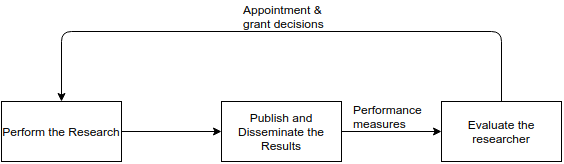
\includegraphics[width=12cm]{images/publication_process.drawio.png}
\caption{Publish for incentives (adapted from~\cite{BH2004})}
\label{fig:publish_incentives}
\end{figure}
% ==============================================================================

In this image we see that the researcher is evaluated and receives incentives 
(such as funds) based on performance measures. In their paper,  Bj\"ork and 
Hedlund mention that for public bodies that provide funds (which is an incentive 
for the researcher), the production and consumption of publications should be 
optimized.
% For researchers, there are multiple strategies to achieve appointments and grants.
% Interestingly, only one of these is to act honestly, that is, to perform the
%     research and publish results. Dishonest approaches are possible,
%     and may even be more rewarding. In absence of deterrents, the scientific
%     process would be inundated by this.
%     \todo{naar intro}
% Existing deterrents are typically focused on specific forms of dishonest
%     behaviour. However, dishonest behaviour still occurs.
    


%% For an author this is an interesting perspective. What can we consider 
%%     production and what consumption and, for detecting fraud, how can we pretend 
%%     to produce and pretend the work is being consumed. In other words; how can 
%%     one pretend to be interesting and gain incentives.
%%     % \item It is save to consider bringing papers to the public as publication. In this chapter we will dive in how this process looks like and the roles and power involved; who has the power that your work can even be consumed?
Two main targets exists for the production part, (the scientific publication): 
journals (incollection) or 
conferences (inproceeding). While journal publications are the norm in many 
other disciplines, conference publications are common in Computer Science.

The next sections describe these processes from a Computer Science perspective. 
For other disciplines these processes may differ. For example, in CS 
conferences, rigorous peer-review is the norm, with acceptance rates of 20\% or 
less being common\footnote{Acceptance rates of security conferences: \url{http://jianying.space/conference-ranking.html}}; in other disciplines, such strict peer review for conferences is
less common.
    
% In the next section we examine the process in more detail.


% ==============================================================================
\section{Journal publication}
% \outline{
% beschrijvend het process bespreken
% }

First we discuss the process for publishing in a journal. Although the 
exact process may differ across journals, there is a certain common process. We 
tend to describe this common process.

The process of publishing in a journal starts with the author who has a manuscript 
he wants to have published. This can be based on a `call for papers', or on own 
initiative. According to Cormode, the Editor-in-Chief receives the manuscript 
and do a minor check if the paper is good enough for further processing. If it 
is, the further process of handling the paper is assigned to an associate editor 
who also perform some checks for quality (understandability, duplication of 
prior work, topic in scope). The checks from the editor-in-chief and associate 
editor can lead to a rejection of the manuscript. According to Cormode, the 
author is encouraged to suggest an associate editor at submitting~\cite{C2013}.
This helps the editor-in-chief to delegate the handling to a associate-editor with knowledge of the domain e.g..

The main responsibilities of the associate editor are 1) initial handling and 
selecting reviews for the papers and 2) obtaining a decision for a paper. 
Although selecting reviewers to review a manuscript is a responsibility of the 
associate editor, it is not uncommon for an author to suggest reviewers. 
Sometimes the author even needs to provide reviewers.

After getting the results from the reviewers, the associate editor decides if 
the manuscript needs to be adjusted. Formally the reviewers give an advise, but 
it is up to the associate editor to do the final judgement. If adjustments are 
needed, the author adjusts his manuscript and this needs to be reviewed again. 
This can happen with other reviewers. An alternative path is that an author 
chooses to withdraw his paper.

\begin{wrapfigure}{r}{0.27\textwidth}
    \centering
    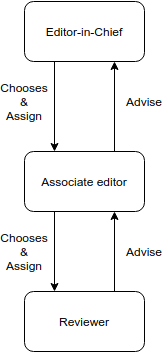
\includegraphics[width=0.27\textwidth]{images/c2013.drawio.png}
    \caption{Roles within the journal process (visual interpretation of description in~\cite{C2013})}
    \label{fig:c2013}
\end{wrapfigure}

Eventually, hopefully, if the paper is accepted by the associate editor, an 
advise will be given to the editor-in-chief. Formally the editor-in-chief 
decides if a paper is being published, but most of the time the advise of the 
associate editor is adopted. This chain of advise and assignment is shown in 
Figure~\ref{fig:c2013}. 

Interesting in this schematic overview is the absolute 
power of the Editor-in-Chief. The person in this role can make a judgement without the advise of the 
associate-editor (and reviewers). Also this role can influence the process by 
choosing a specific associate-editor. Under the Editor-in-Chief, we draw the 
Associate editor. This role has two ways to influence the process; by choosing 
the reviewers and by giving the advise to the editor-in-chief. The reviewers 
have less power; off course they can provide an advise, but most of the cases 
there are multiple reviewers.


% \begin{figure}[H]
% \centering
% 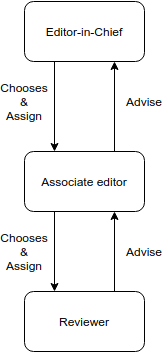
\includegraphics[width=3cm]{images/c2013.drawio.png}
% \caption{Roles within the journal process (visual interpretation of description in~\cite{C2013})}
% \label{fig:c2013}
% \end{figure}
% \outline{
% wordt zo en zo laten zien in in BH
% }
% ==============================================================================
To visualise the publication process for journals, we can use a model of 
Bj\"ork and Hedlund. They modelled the various processes involved in scientific
publishing to investigate the business impact of the shift towards internet
publishing models. This model is based on publication for journals.
For our research, we took a diagram from their publication and took the 
activities usable for our research. Hereby neglecting the steps 
"Negotiate copyright" and "Copyedit Article". The result is shown in 
Figure~\ref{fig:bh2004_a22331}.

\begin{figure}[H]
\centering
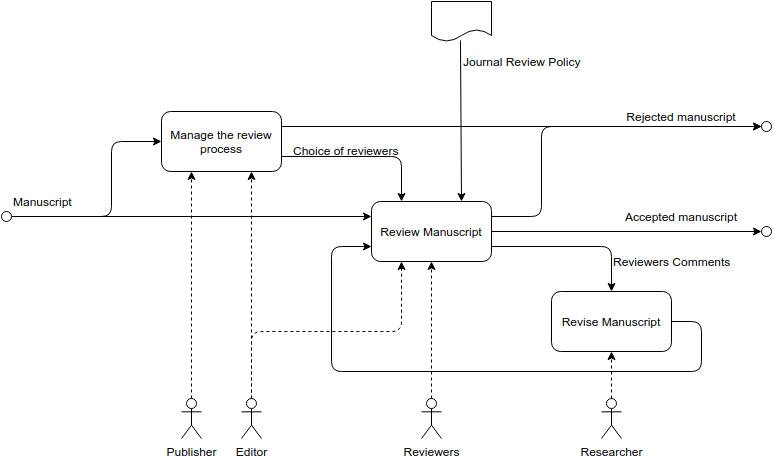
\includegraphics[width=14cm]{images/bh2004_dia_a22331_part.drawio.png}
\caption{Journal process flow between submission and decision (adapted
from~\cite[diagram A22331]{BH2004})}
\label{fig:bh2004_a22331}
\end{figure}
% ==============================================================================
The phase "Manage the review process" from Bj\"ork and Hedlund is described by 
Cormode from the perspective of the Editor-in-Chief and Associate editor (Bjork 
and Hedlund decided to use one role: editor). 


% ==============================================================================
\section{Conference publication}
The following is an informal description of the process for conference 
publication which can also be a workshop or symposium. Not all conferences 
follow this approach. Input for this description is provided by the supervisor
of this research project.

For established venues the steering committee decides to have a conference and 
choose a location. The main responsibility of the steering committee is to 
oversee the organisation of the conference and choosing the program 
committee (PC) chairs which responsibility is to compose a program out of a 
subset of the received 
submissions. For new subjects, the trigger comes from one or more 
academics who thinks a conference is needed for a certain subject and try to 
form a Program Committee (PC). 

Possibly there are ``program tracks'' on specific subjects, with dedicated
chairs for each track.
% ============================================================================== 
The PC chairs invite people to become program 
committee members. A new trend is self-nomination; one can nominate himself for 
a position in the program committee. Another new trend is that authors of 
submitted papers are required to review.

Besides inviting members, the PC chairs ensure the website is up, promotion 
is in place and have submission/review server set up.
The PC chairs create and distribute a call-for-papers, which starts the 
\textbf{submission phase}.
% ============================================================================== 
Responding to the call-for-papers, scientists submit papers, and possibly 
marking conflict of interest. 
% Likely, PC Chairs extend deadline, which gives 
% more scientists the possibility to submit papers. 
After a likely extension of the deadline, PC Chairs close submission and 
perform desk reject.
% ============================================================================== 

After the submission phase closes the \textbf{bidding phase} begins. During 
this bidding phase, PC members bid on which papers they would like to review.

In the \textbf{review phase} the PC members read and score the papers. In this 
phase a paper can be early rejected with limited number of reviewers. Sometimes 
this phase contains a rebuttal phase; the reviews are send to authors so the 
authors can reply on the given comments.

In the following \textbf{discussion phase} the PC member unify their views about 
the papers. After the discussion a decision should be made.

During the \textbf{decision phase} the PC Chairs formalise a decision about a 
paper (formally; often they simply follow the consensus view). Possible 
decisions are accept, reject or conditionally accept (shepherding). In this 
case, the paper is interesting but not yet quite acceptable, salvageable. One 
reviewer is designated Shepherd and communicates with the authors on what 
changes are needed. Final acceptance hinges on the Shepherd officially 
approving the paper.

In the \textbf{camera-ready phase} the authors make final changes, 
incorporating editorial changes, reviewer comments, etc., and submit the final 
version for publication.

In the \textbf{publication phase} the PC chairs judge on the the camera-ready 
version, and papers is published online.
% ============================================================================== 


% \outline{
% \begin{itemize}
%     \item wat is macht program committee vs program chair; 
%     \item Conferentie, core ranking: https://www.core.edu.au/conference-portal
    
% \end{itemize}
% }

% \newpage
% \subsection{Model of proceedings}
% \begin{figure}[htbp]
%   \begin{center}
%         \begin{tikzpicture}[
%             auto,node distance=5cm,thick,
%             rolenode/.style={circle, draw=green!60, fill=green!5, very thick, minimum size=1.05cm},
%             thingnode/.style={rectangle, draw=red!60, fill=red!5, very thick, minimum size=1.05cm},
%             ]
%             % Nodes
%             \node[rolenode] (sponsoring_organization) {SO};
%             \node[rolenode] (general_chair) [below=of sponsoring_organization] {GCh};
%             \node[rolenode] (general_committee) [below=of general_chair] {GCo};
%             \node[rolenode] (program_chair) [below=of general_committee] {PCh};
%             \node[rolenode] (program_committee) [below=of program_chair] {PCo};
%             \node[rolenode] (reviewer) [right=of program_committee] {R};
%             \node[rolenode] (steering_committee) [right=of general_chair] {SC};
            
            
%             \node[thingnode] (conference) [right=of general_committee] {Conference};
%             \node[thingnode] (proceeding) [below=of conference] {Proceeding};
%             \node[thingnode] (paper) [below=of proceeding, right=of reviewer] {Paper};
%             \node[rolenode] (author) [right=of proceeding] {A};

            
%             % Lines
%             \draw[->] (sponsoring_organization) -- node [text width=2.5cm,midway,above,sloped] {appoints} (general_chair);
%             \draw[->] (general_committee) -- node [text width=2.5cm,midway,above,sloped] {organizes} (conference);
%             \draw[->] (general_chair) -- node [midway,above,sloped] {assembles} (general_committee);
%             \draw[->] (general_committee) -- node [midway,above,sloped] {contains / advises for members} (program_chair);
%             \draw[->] (program_chair) -- node [text width=2.5cm,midway,above,sloped,align=center] {assembles} (program_committee);
%             \draw[->] (program_committee) -- node [text width=2.5cm,midway,above,align=center] {assigns} (reviewer);
%             \draw[->] (conference) -- node [text width=2.5cm,midway,above,sloped] {leads to} (proceeding);
%             \draw[->] (proceeding) -- node [text width=2.5cm,midway,above,sloped] {contains} (paper);
%             \draw[->] (reviewer) -- node [text width=2.5cm,midway,above,sloped] {reviews} (paper);
%             \draw[->] (author) -- node [text width=2.5cm,midway,above,sloped] {writes} (paper);
%             \draw[->] (steering_committee) -- node [text width=2.5cm,midway,above,sloped] {plans} (conference);

%         \end{tikzpicture}
%   \end{center}
%   \caption{Publication process for collections.}
%   \label{fig:structure}
% \end{figure}

% ==============================================================================
\section{Fraud in the publication process}
\label{sec:domain_analysis:fraud}
% \outline{
% \begin{itemize}
%     \item Domain
%     \item Impact van process Welk effect heeft publiceren
%     - \# publicaties
%     - \# citaties
%     - kwaliteit
%     \item beter doen levert voordelen
%     \item dus zijn er incentives voor valsspelen
%     \item Idee\"en egregious examples -> als deze situatie voorkomt, wil ik 
%     het vinden
% \end{itemize}
% }
% ==============================================================================
In the introduction we already referred to the aphorism known as Goodhart’s Law 
: ``When a measure becomes a 
target, it ceases to be a good measure''~\cite{strathern_1997}. Known metrics 
such as the H-Index not only incentivise scientific 
excellence; they also invite other ways to achieve high rankings (e.g. 
plagiarism, manipulation of images, manipulation of research data, 
fabrication of research data). 



% The underlying assumption is
% that the various types of scientific fraud all share a common characteristic: 
% their goal is the same, that is, their goal is to improve a researcher’s or 
% publication’s quantitative measures of science. This elevates them above their 
% peers – which on the one hand brings recognition and accolades, but on the other, 
% it makes them stand out. In short, the underlying
% assumption is that fraudsters aim to become outliers (in terms of quantitative measures of
% science).


% \outline{
% \begin{itemize}
%     \item probleem -> valsspelen
%     \item - wat is dat
%     \item - op oneigenlijke gronden
% \end{itemize}
% }
% ==============================================================================
% Examples already mentioned in the introduction are plagiarism, manipulation of 
% images (e.g., of cell 
% extracts in life science publications), manipulation of research data, 
% fabrication of research data. In addition, there may be as-of-yet unknown forms 
% of fraud.

% \outline{
% \begin{itemize}
%     \item dan interessante gevallen
% \end{itemize}
% }
% The this section we elaborate on an interesting case that may contain fraud.
% Furthermore, during the case studies we will provide some other examples.
This section provides short description of some interesting cases that may 
occur in the above described processes.
It is certainly not the case that all situations do actually imply fraud, but 
these are cases that are a candidate for further manual investigation.
Here we do not mention content-based fraud like plagiarism, we focus on fraud
during the publication process. As Mario Biagioli calls them `post-production 
misconduct', which is probably a nicer term~\cite{biagioli2020gaming}.

\paragraph{Publications cites publications in the same venue} It is remarkable
if a venue cites only work from itself. The benefit for this venue is that it
increases the impact score of the venue. This case is described as an example in 
Section~\ref{interesting_case:publications_cites_publications_in_same_venue}.
% ==============================================================================
\paragraph{Work member of editorial board is being cited} Member of the
editorial board that is excessively often being cited in his own venue, can be
an indicator for fraudulent behaviour. This case serves as input for case 
study~1 (Chapter~\ref{chp:case1}) and is described further in 
Section~\ref{interesting_case:work_member_editorial_board_cited}.
% ==============================================================================
\paragraph{Member of the editorial board is (co-)author} 
A questionable situation occurs if a member of the editorial board becomes co-
author of \textit{relatively} a lot of publications. This may indicate that 
authors are being forced to add the member to the author list. The benefit for
the member increasing his publication count and, if the article gets cited, 
citation count (which has impact on the H-Index and therefore impacts his 
career).

This situation is described in case study 2
(Section~\ref{interesting_case:member_editorial_board_is_coauthor}).

% ==============================================================================
\paragraph{Author reviews his own work}
This kind of fraud is known because of Moon. Moon gave an e-mail address of 
himself (alias) as reviewer for his own work. This case was detected because of
the short time between submission and accordance. Moon was detected, but are 
other authors that show this fraudulent behaviour also detectable?
Case study 3 (Chapter~\ref{chp:case3} is based on the publication-lag (time 
between submission and publication of an article).

\paragraph{}
Off course possible fraudulent behaviour is not limited to these cases. Other 
cases are
described on the website of COPE (Committee on Publication Ethics)\footnote{\url{https://publicationethics.org/guidance/Case}}.

\section{Conclusion}
In this chapter we described the processes to publish 
articles for journals and conferences. In these processes fraud can be conducted,
which we have shown with a few cases.

The information in this chapter is domain knowledge which is needed to conduct 
this research.

% \section{Interesting cases}
% \label{interesting_cases}
% In this section we describe theoretical and practical (actually happened) 
% attacks on the integrity of the publication process. We can use these attacks to 
% complete the theoretical (or logical) publication model.



% \outline{
% \begin{itemize}
%     \item The articles of a journal that are cited impact the journal impact factor.
%     \item It is important that this number is high.
%     \item Meetbaar door de verhouding te bekijken van de journals waar de geciteerde artikelen uit komen.

%     \item In praktijk al Thomson
%     \item Verwachting is niet veel op vinden
%     \item deze laten zitten
%     \item als voorbeeld hoe de modellering werkt
% \end{itemize}
% }


% \subsection{All time favourite: Diederik Stapel}
% % ------------------------------------------------------------------------------
% \vraag{Wat met Diederik Stapel?}
% \outline{ergens in het begin: er zijn manieren om te frauderen...}

% The fraud that Diederik Stapel committed was not related to the publication 
% process, but to the data he used to draw conclusion on.
% With our specific method, we will not be able to detect data manupulation and
% fabrication.
% However the \textit{effect} of his approach is a lot of publications.

% \outline{door neven effect van fraude (bijvoorbeeld heel veel publicaties) of 
% zijn resultatenn halen het nieuws / opgemerkt in academische wereld omdat ze 
% fout zijn / omdat heel veel citaties eerste maanden zijn}.

% ------------------------------------------------------------------------------

% \outline{
% \section{placeholder}

% \begin{itemize}
%     \item Author and reviewer are the same person: $\{h \in \Humans \mid \authors(p, h) \land \reviews(p, h)\}$ (Moon)
%     \item Editor-in-Chief is part of authors: $\{h \in \Humans \mid \authors(p, h) \land \receives(p, h)\}$. Logisch gevolg is dus dat $\accepts(p, h)$
%     \item Citaat naar paper van iemand in het proces: stel q is de publicatie waar het om draait dan:
%     $\{h \in \Editors \cup \Reviewers \mid \cites(q, p) \land \authors(h, p)\}$
%     \item bovengemiddeld zelfcitaties
%     \item publicaties die geciteerd worden komen uit dezelfde journal
% \end{itemize}
% }

% \outline{
% \begin{itemize}
%     \item dan modellering (hfst \ref{chp:modelling_the_publication_process})
% \end{itemize}
% }

% ==============================================================================
\chapter{Related work}
\label{chp:related_work}
% ==============================================================================
% \outline{
% \begin{itemize}
%     \item Tielenburg in lead
%     \item gebasseerd op model JM (laten zien)
%     \item Afzonderlijke stappen beschrijven
%     \item Hij vond resulaten maar...
%     \begin{itemize}
%         \item Niet over alles
%     \end{itemize}
% \end{itemize}
% }
%% He manually developed three heuristics. Although each
%% heuristic where three 
%% manually heuristics are proposed to identify outliers~\cite{TEJ2017}. As data 
%% sources DBLP and Google Scholar were used; datasets in this study contained data 
%% about publication, author, venue and, in the case of Google Scholar, citations. 
% ==============================================================================
% \todo{
% \begin{itemize}
% \item Tielenburg17: 
%     \begin{itemize}
%     \item more generic approach needed
%     \item generic outlier detection on JM17 data insufficient
%     \item suggestion: extension of JM17 needed
%     \end{itemize}
% \end{itemize}
% }

As stated in the introduction; a more generic approach for fraud detection is 
needed. This research is a continuation of the research of 
Tielenburg, which tried to apply this generic approach~\cite{TEJ2017}.

\begin{wrapfigure}{r}{0.25\textwidth}
    \centering
    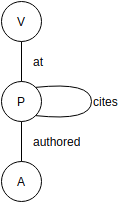
\includegraphics[width=0.25\textwidth]{images/jm2017_undiced_pub_view.drawio.png}
    \caption{Set-theoretic publication model adapted from~\cite{JM2017} used 
by~\cite{TEJ2017}}
    \label{fig:rw_jm2017}
\end{wrapfigure}

Tielenburg investigated automated detection of fraud-like behaviour based on
publicly available data ga\-thered from DBLP and Google Scholar. He determined 
fraud indicators based on a data model of the publication process proposed by 
Jonker and Mauw~\cite{JM2017} shown in Figure~\ref{fig:rw_jm2017}. In this 
model \textit{V}, \textit{P} and \textit{A} stand for Venue, Paper and Author.
% \begin{figure}[H]
% \centering
% 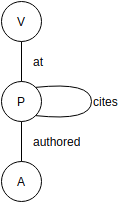
\includegraphics[width=3cm]{images/jm2017_undiced_pub_view.drawio.png}
% \caption{Set-theoretic publication model adapted from~\cite{JM2017} used 
% by~\cite{TEJ2017}}
% \label{fig:rw_jm2017}
% \end{figure}




Tielenburg proposed three heuristics calculated about the authors to identity 
outliers: 
\textit{maxdiffpubcount} (maximum over the difference in the number of 
publications between two consecutive years), \textit{maxdiffcitecount} (maximum 
over the difference in the number of citations between two consecutive years) 
and \textit{maxratiocitsvspubs} (maximum of the ratio between citations and 
publications). The latter is a derived value based on publication 
and citation counts per year.

Tielenburg's implementation based on the data modelled by Jonker and Mauw was 
not successful. Therefore, this model needs to be extended.

\paragraph{Extending the model}
% \todo{
% \begin{itemize}
% \item What extensions are needed:
%     \begin{itemize}
%     \item Haug15: editors, reviewers
%     \item Bishop: editors
%     \item Scanff: editorial board, publication lag
%     \end{itemize}
%     \ldots
% \end{itemize}
% }

Haug raised attention to fraud in the peer-review process and the important role
(guest-)editors have in relation to the peer review process~\cite{Haug2015}. The 
attacks she presents are self reviewing like Moon and Chen and fake reviewers.
Another attack she mentions is the attack on the systems supporting the peer-review
process.

Bishop\footnote{\url{http://deevybee.blogspot.com/2020/07/percent-by-most-prolific-author-score.html}}
additionally considers the impact of the role of the editor.
In her blogpost she raises attention to members of the editorial board which are
also co-authoring articles. However, this is mainly focuses on one editor.

Scanff et al.~\cite{SNCMBL2021} focused on the publication process of prolific
authors, who might be part of the editorial board. They measured the
publication time (time between submission and acceptance) of these prolific
authors and noticed how this period is less for papers written with prolific
author compared to papers written without prolific authors. 


\paragraph{Filling the model}
% \todo{
% \begin{itemize}
% \item How to fill the model:
%     \begin{itemize}
%     \item CPN21: data on specific roles needed, but not readily available.
%     \item Ley09: DBLP: JM17 w/o citations
%     \item HPS19: OpenCitations: doi2doi data
%     \item TZY08: Aminer: JM17-alike
%     \item Conclusion: no complete dataset available $\to$ data acquisition needed.
%     \end{itemize}
% \end{itemize}
% }
% However, investigations into the impact of specific roles require availability of
% the underlying data. 
Chakraborty et al.~\cite{CPN2021} found data on the various
roles in the publication process lacking to such an extent, they could not complete
their originally envisioned research. Thus, while specific roles may significantly
impact the publication process, data regarding these roles is not readily available.
Data acquisition is thus a key component of any study into the correlation between
specific roles and impact.

\textbf{\dblp{}} is a publicly available dataset focused on publications in the
Computer Science Domain. The dataset contains publications, authors and venues.
Ley descibes the choices made by \dblp{} composing the
dataset~\cite{DBLP:journals/pvldb/Ley09}. The person entity is described in 
detail included the procedure DBLP takes to identify unique people with the same
name or an author with multiple names.
The data \dblp{} uses to create this dataset is being pushed from publishers or 
scraped from the web using web crawlers. \dblp{} covers the datamodel of Jonker
and Mauw without the citations.

Heibi et al. introduced the \textbf{OpenCitations} COCI (Crossref OpenCitation 
Index) dataset. This dataset contains citations on DOI-to-DOI
based~\cite{DBLP:journals/scientometrics/HeibiPS19}.
OpenCitations acquired their data from undisclosed datasources.

Aminer is a service that provides datasets for analysis of the publication
process.
Tang et al. descibed how \textbf{Aminer} loads the source data from sources and 
uses probablistic models to deal with name disambiguity~\cite{Tang:08KDD}. As 
with DBLP, Aminer also elaborates on how they tackle the author-naming problem.
The citation dataset, which contains authors, publications and citations, uses
data from DBLP, ACM and `other sources'. 
Aminer covers the model from Jonker and Mauw, focused on citations. However,
for the entities involved, a lot of attributes are not available.

\ \\
As conclusion, no complete dataset is available. Therefore, we need to acquire 
additional data.


\paragraph{Data acquisition and parsing}
% \todo{
% \begin{itemize}
% \item Data acquisition:
%     \begin{itemize}
%     \item some data publicly available in PDF or HTML form
%     \item Acquiring data from HTML: crawl site; parse \& store data.\\
%         Similar to: \cite{one, two, three}
%     \item Acquiring data from PDF: crawl sites; download PDF; parse PDF;
%         store data. \\
%         Similar to: \cite{fourfivesixseven,whoshallI,giveakoessie}
%     \end{itemize}
% \end{itemize}
% }
As described in previous paragraph, the actual source data used to create public datasets
is not transparent. However, generally we notice that the most `original' 
data (not acquired from other public datasources) is acquired from websites of 
publishers (e.g. using the webcrawlers in case of \dblp{}). 

Besides websites, publications and
editorials are most of the time available in PDF format. Therefore we focus in this 
paragraph on acquisition which contains `downloading' the content (which may be 
HTML of PDF) and parsing, transforming the acquired data in information.

For downloading content from the web (e.g. HTML or PDF documents) standard tooling 
exists (e.g. cURL\footnote{\url{https://curl.se/}}, 
wget\footnote{\url{https://www.gnu.org/software/wget/}}). For incorporating this downloading in software, multiple
libraries exist.

In case of HTML two type of methods for acquiring content exist: web browser wrappers 
(e.g. Selenium) and HTTP libraries (e.g. Urllib2)~\cite{zhao2017}. The first 
simulates a browser. The advantage is that dynamic content can also be acquired. 
The second is a single GET request (which is equivalent to tooling described before).

The content acquired differ from site to site. Therefore, this content needs to be
interpreted to turn this acquired data into information.

\ \\
Parsing is extracting information from the acquired (raw) data. The parsing 
mechanism depends on the type of data.  Examples are HTML (web pages), datafeeds 
in XML and JSON or multimedia types. Considering the type of data his research 
is conducted on, we focus on HTML and PDF files.

Zhoa~\cite{zhao2017} mentioned BeautifulSoup for interpreting HTML and Pyquery
for XML. Uzun et el.~\cite{uzun2018comparison} comparised regex and DOM-based 
libraries (Lxml and BeautifulSoup) for data parsing. DOM-based libraries were 
better for parsing than using regex.

Lo et al. interpreted PDF's from multiple papers \cite{lo-etal-2020-s2orc} to 
extract bibliographic information. They also tried to parse Latex documents, but
surprisingly, the results were worse with Latex then with PDF. For extracting 
information from PDF's, they relied on a project called
ScienceParse~\footnote{\url{https://github.com/allenai/science-parse}}. This is 
framework that interprets Scientific Papers. The main component used to read the
PDF documents, is PDFBox.
This parsing of PDF's is similar to \cite{niu2014realization} and \cite{BK2017}.
% Niu et al. also extracted information from papers \cite{niu2014realization}.
% For extracting text from PDF's multiple studies are conducted for interpreting 
% scientific papers \cite{niu2014realization}, \cite{BK2017}.

% Bast and Korzen performed a benchmark of tools for extracting text from PDF 
% documents. Considering the error-rate of various tooling, pdftotext, pdftohtml, 
% pdftoxml, pdfbox and parscit are considered the top 5 tools~\cite{BK2017}.

% Hashmi et al. provided an overview with possible methods to extract 
% information from the text. They describe the Machine Learning, Rule-based and 
% hybrid approaches \cite{hashmi2020insights}.



% ------------------------------------------------------------------------------
\paragraph{Modelling the publication process} \label{rw_publication_process}
% ------------------------------------------------------------------------------
For integration of multiple datasources, we need a model of the publication 
process.

We already mentioned the set-theoretic publication model presented by 
Jonker and Mauw~\cite{JM2017}, shown in Figure~\ref{fig:rw_jm2017}. This model
is used to formulate an attack surface on the publication process. However, 
based on work from Tielenburg, Haug, Scanff et. al. and Chakraborty et al. we 
can conclude that this model is insufficient to detect fraud; necessary data can 
not be added to this model.

% ==============================================================================
Björk and Hedlund~\cite{BH2004} describe a  model of the publication process
for measuring costs. Their model includes a large set of involved entities
and roles. While this model provides a solid foundation for understanding the
publication process, the model is a process model and does not facilitate
deriving publication metrics. As such, it is unsuited for determining
the value of quantified fraud indicators.

% ==============================================================================
From the view of the associate-editor, Cormode describes in detail how his work
looks like~\cite{C2013}. It provides a good insight of the work of an associate 
editor, which can also be read from an 'attacker-mindset' (where are the 
vulnerabilities), but unsuited for fraud detection.

% ==============================================================================



% ==============================================================================
% \paragraph{Fraud indicators}
% \outline{andere onderzoeken naar fraude}
% \outline{
% \begin{itemize}
%     \item Scannff
%     \begin{itemize}
%         \item Subgroep werken werkt wel
%         \item data niet toereikend
%         \item Conclusie: er kan wel iets
%     \end{itemize}
% \end{itemize}
% }




% ==============================================================================




% ==============================================================================




%% In particular, they could not investigate 
%% \textit{author-editor affiliation analysis} nor \textit{editorial board 
%% composition}.

%% present features to enable outlier detection for unethical 
%% citation practices~\cite{CPN2021}. Their focus is the domain of Computer Science.
%% A k-means clustering is applied to the proposed features which resulted in some
%% extreme outliers. Their next focus is to explore other features. Two future 
%% directions are interesting and related with previous mentioned work; 
%% \textit{author-editor affiliation analysis} and \textit{editorial board 
%% composition}. The reason 
%% they were unable to add this to their current study, is lack of data 
%% availability.

% \ \\
% From the above described work we notice interesting points:
% \begin{itemize}
%     \item Working with groups (\cite{SNCMBL2021}) instead of the whole 
%         population (\cite{TEJ2017}) may work;
%     \item Data used by~\cite{SNCMBL2021} contains additional attributes not 
%         available in the datasets (DBLP and Google Scholar) used by Tielenburg;
%     \item The editor is a real necessity to include in datasets regarding the 
%         publication process.
% \end{itemize}


% ==============================================================================
% Data is needed to apply fraud detection. 




% ==============================================================================


% ==============================================================================



% ==============================================================================

% \paragraph{}
% A first insight we gain from this 
% model is that how the publication process can be played depends on the role of 
% the fraud; e.g. an editor has other possibilities than a reviewer. We can 
% expand the model further by adding the review process. Ali and Watson describe 
% different types of review processes and their advantages and 
% disadvantages~\cite{AW2016}.

% As 
% mentioned in Section~\ref{sec:problem_statement} we consider this dataset too limited. 

% We 
% challenge this 
% research and want to apply detection of outliers on a dataset which contains
% additional entities.
% Tielenburg proposed three heuristics calculated about the authors:
% \textit{maxdiffpubcount} (maximum over the difference in the number of 
% publications between two consecutive years), \textit{maxdiffcitecount} (maximum 
% over the difference in the number of citations between two consecutive years) 
% and \textit{maxratiocitsvspubs} (maximum of the ratio between citations and 
% publications). The latter is a derived value based on publication 
% and citation counts per year. 
% We think this approach failed because of the lack of data and the 

% Because it combines two raw values we choose not 
% to use this one. The first two metrics, however, may be interesting; we need to 
% fit raw values in a number to be used by an algorithm and this aggregation can 
% be an option.

% However, publication and citation counts may not be the only metrics to identify 
% fraud. To discover other metrics identifying gamification of the publication 
% process, we need to formalise the model of this process. 


% % ------------------------------------------------------------------------------
% \paragraph{Fraud in the publication process}
% % ------------------------------------------------------------------------------
% The publication process is played by unforeseen attacks, attacks which are not 
% identified and without countermeasures. Jonker and Mauw presents a way to see 
% how metrics can be played, using a formalised model~\cite{JM2017}.
% In an audio interview Dr. Haug raises attention to fraud in the peer-review 
% process with the change that the internet has brought\footnote{\url{https://www.nejm.org/doi/full/10.1056/nejmp1512330}}. She 
% presents some attacks in this interview and make the role and responsibilities 
% of the editor a central item. The role of the editor is also being considered 
% important by 
% Bishop\footnote{\url{http://deevybee.blogspot.com/2020/07/percent-by-most-prolific-author-score.html}}.
% In her blogpost she raises attention to members of the editorial board which are




% ==============================================================================
\chapter{Methodology}
\label{chp:methodology}
% ==============================================================================
In Chapter~\ref{chp:domainanalysis} we described the processes to publish 
articles for journals and conferences. In these processes fraud can be conducted.

To improve detection of this fraud, data about these processes is necessary.
Previous approach (\cite{TEJ2017}) to discover fraudulent behaviour was based 
on public datasets, but misses important entities. 

Considering the cases described in Section~\ref{sec:domain_analysis:fraud} and 
public datasets that are generally represented by Jonker and Mauw~\cite{JM2017},
missing entities can be pointed out.
In Figure~\ref{fig:jm2017_missing_ent} the generic data model for public 
sources is on the right side; V for venue, P for paper and A for author. Left of 
this model missing entities are added.

% \begin{wrapfigure}{r}{0.5\textwidth}
%     \centering
%     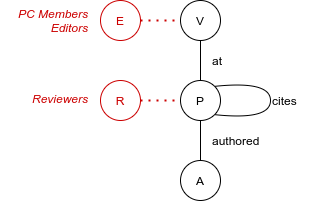
\includegraphics[width=0.5\textwidth]{images/jm2017_miss_ent.png}
%     \caption{Right: Set-theoretic publication model adapted from~\cite{JM2017} Left: Missing entities considering example attacks.}
%     \label{fig:jm2017_missing_ent}
% \end{wrapfigure}

\begin{figure}[H]
\centering
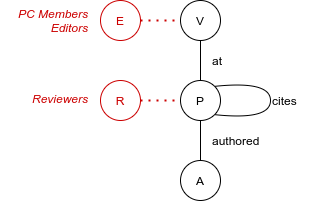
\includegraphics[width=7cm]{images/jm2017_miss_ent.png}
\caption{Right: Set-theoretic publication model adapted from~\cite{JM2017} Left: Missing entities considering example attacks.}
\label{fig:jm2017_missing_ent}
\end{figure}

However, these missing entities are available, but not in a structured format and
integrated in existing datasets. This brings us to the main question of this research:

% In this research we want to investigate 
% how the integration of public data coming from different sources improves the 
% detection of scientific fraud.

% The main question we want to answer with this research is: \\
\ \\

\textbf{How can integration of public available data sources improve the detection of scientific fraud?} \\

% Tielenburg tried to apply outlier detection on the whole population, 
% without success. This does not mean outlier detection will not work with integrated 
% additional data.

Our assumption is that a group based approach will improve the detection. 
Therefore we need data to identify these groups. As we know from our research 
proposal, public available datasets do not contain necessary information to 
identity groups. Therefore, data to apply group identification needs to be 
acquired from additional sources and integrated with other existing datasets. 
To determine which data we need, a datamodel of the publication process is 
required.

This reasoning implies the following approach:
\begin{enumerate}
    \item Define the datamodel for the publication process
    \item Acquire and intergrate data to fill this datamodel
    \item Apply group based outlier detection
\end{enumerate}

\paragraph{Define datamodel}
Missing entities are mentioned in the problem described in the lead of this 
chapter. The resulting figure
(Figure~\ref{fig:jm2017_missing_ent}) is not sufficient to build a dataset 
for fraud detection. Therefore, as first step a more concise datamodel is needed
to enable detection of interesting cases. With this step we identify entities
and their relations.

Possible approaches to define a datamodel are:
\begin{description}
    \item[1. Use an existing datamodel] Datamodels about the publication process
    do exist. An initial analysis made clear that existing models are
    somehow limited to the author, venue and publication. Attacks as described
    in Section~\ref{sec:domain_analysis:fraud} are not possible to detect using 
    these models. As an example: the Microsoft Acadamic Graph 
    model\footnote{\url{https://docs.microsoft.com/en-us/academic-services/graph/reference-data-schema}} 
    (which is the most detailed we came across) does not contain any other role 
    than author.
    \item[2. Create a model]  The domain analysis can be used as input to create
    a datamodel.
\end{description}

A combination of these approaches will add the most value for this study. The 
reason is that existing models have a good starting point. However, some 
extensions are needed for our study. 

We scope this step by modelling a logical model. There are two reasons for this:
\begin{enumerate}
    \item An physical model containing all possible attributes is too 
        detailed. Taking this approach will take too much time while the added
        value is not worth the effort.
    \item By using a logical model, the focus is on the entities and their
        relations. These are the most important components for a group based
        detection.
\end{enumerate}

This does not neglect the need for a physical model for implementation. 
Multiple physical modelling techniques exist which can be used for 
implementation.
% By using a more high-level logical model approach, we can define a model 
% focused on the entities and relations involved, which can be implemented 
% using multiple physical modelling techniques. 


\paragraph{Acquiring and integrate data}
The second step is to determine which publicly available dataset can (partially) 
fulfill some parts of the model defined in the previous step. Our approach is here to 
discuss the available datasets and how these covers the model.

Based on the research preparation, we know \dblp{} and Aminer are two sources
that we probably can use. In this step a more extensive investigation is 
needed focused on integration and covering entities and relations from the 
resulting model from the first step.

Sources for required entities not covered by public datasets should be found. 
For every source we should investigate the following points:

\begin{itemize}
    \item How the acquisition will take place. This depends on the source.
    \item How integration of this newly acquired data should take place. This 
        depends on available attributes.
\end{itemize}

An approach for these added sources can not be decided up front.

% ============================================================================

\paragraph{Apply group based outlier detection}
In this step we define groups and apply a group based detection on the dataset
composited from the previous step.

% options

% Our approach is to execute case studies base on groups identified in cases 
% described in Section~\ref{sec:domain_analysis:fraud}.



% Alternative approach would be to acquire data, create one integrated dataset, 
% followed by applying outlier analysis on this dataset. 
% But there are a few reasons not to do this:
% \begin{itemize}
%     \item 1) Not all data is available of all entities. Some data is hard to 
%     acquire and not gene\-rally available. We need to
%     execute a case study on a certain group where this data is available for.
%     As we only consider the group where we were able to get the data for, a 
%     more reliable analysis can be conducted. Our purpose is to demonstrate that it is 
%     rewarding to integrate datasets; not to get this data for the whole population.
%     \item 2) Our defined attacks are all 'related to'; compared within a group of
%     peers. This also implies the need for a group based approach (e.g. group 
%     of editors).
%     \item 3) Tielenburg tried to apply outlier detection on the whole population, 
%     without succes. This does not mean his approach will not work with integrated 
%     additional data. However this study we take a step back; add additional data 
%     for a group and perform outlier analysis within this group. An approach 
%     involving the whole set is probably too soon; first investigate if additional 
%     data improves the detection (this study), then acquiring the data for the 
%     complete set and maybe then a research can be conducted on applying outlier 
%     analysis on the whole set (Tielenburg).
% \end{itemize}

% \paragraph{Case studies}
% We mentioned case studies in the previous paragraph. 
In the domain analysis of the 
publication process interesting situations are 
described with the groups having the power to abuse that particular situation
(Section~\ref{sec:domain_analysis:fraud}). In Figure~\ref{fig:research_method} this
is these are represented with the arrows from the publication process to the roles.

\begin{figure}[H]
\centering
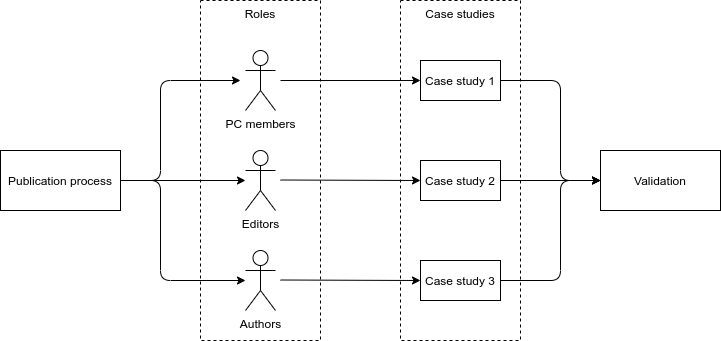
\includegraphics[width=13cm]{images/research_method/research_method.png}
\caption{Relation publication process, roles and case studies}
\label{fig:research_method}
\end{figure}
Based on these situations three cases studies (identifiable groups) are formulated:
\begin{itemize}
    \item Program Committee Members
    \item Editors of a journal
    \item Authors
\end{itemize}

For every use case we do the following:
\begin{itemize}
    % \item Acquiring the additional data (if not already acquired by the previous steps);
    \item Create an analysis dataset from the previous step focussed on
    this group and its metrics;
    \item Validate possible interesting cases.
\end{itemize}

% To answer the question (how can we identify possible fraudulent 
% behaviour in a specific group of peers) involves a structured approach.
% First we need to formulate a dataset to perfrom the analysis on. At forehand
% we do not know if the datasets available from public sources are sufficient enough.

% During these case studies we will need to answer some questions:
% Why is this an interesting group to analyse?
% Is the dataset from RQ1 sufficient to analyse this group?
% If we need additional data, what is the availability of this data?
% And how can we integrate this data to perform outlier detection.

\paragraph{Formalising the conclusion}
The combinations of validations from the case studies will result in the
answer on the question if acquiring and integrate publicly data improves
the detection of scientific fraud.


% \outline{
% Belangrijkste punten:
% \begin{itemize}
%     \item Wat ga je doen?
    
%     We will do this by:
%     - Creating a model of the publication process that is extensible with other data related to the publication model and investigate how we can fill this with existing datasets.
%     - 
    
    
%     Approaches for validation:
%     \paragraph{Peer comparison} This approach contains comparing the `group' with its peers.
    
%     \paragraph{Derived metrics} By calculating metrics of a certain group we could run an outlier detection.
    
%     \paragraph{} We choose the first option. The reasons are:
%     \begin{itemize}
%         \item We want to stay as close to the raw data as possible. Defining derived metrics and apply outlier detection based on these, has been performed by Tielenburg without success.
%         \item 
%     \end{itemize}
    
%     Validation will be executed for every case. Here we will consider the added
%     data as group and determine if this results in outliers.

    
%     \item Waarom ga je dat zo doen?
%     \item er zijn andere manieren: ik kies deze methode want...
%     \item wordt nu gekeken naar input kant -> willen naar effect kijken (output kant, onafhankelijk van input kant)
%     \item tielenburg heeft gekeken groter trekken -> werkt niet, data niet rijk genoeg
%     \item Draait om detecteren of er aanvallen plaats vinden
%     \item Wat hebben we nodig om aanvallen te detecteren (hoe kunnen wij dat 
%     doen?
%     \item Redenering dat we een model nodig hebben
% \end{itemize}
% }

% ==============================================================================
% \section{Research Questions}

% % Hoofdvraag: Heeft outlier detectie binnen een groep zin?
% The main question we want to answer in this research is: \\
% \textbf{What is the impact of using a group-based outlier detection approach in 
% detecting fraud in the scientific publication process?}

% What we want to validate in this research is: \\
% \textit{There exists fraud in the publication process which causes fraudsters
% to become detectable outliers with respect to their peers.}


% The statement we want to verify with this study is:
% People with malicious ways to accomplish improvement of their quantitative 
% measures, will be an outlier compared with their peers.

% Hypothese: Door breder trekken van data zijn we wel in staat om outliers te detecteren

% Vraag: waar schiet het model te kort
% ant: in praktijk deze aanvallen -> deze data nodig -> niet beschikbaar in databronnen

% identificeren attributen
% data bronnen
% acquisitie
% integratie

% We define the following subquestions:

% \begin{enumerate}[label=RQ\arabic*]

%     \item \label{RQ1} \textit{How can we define a dataset from known public 
%     datasources to populate a formal publication model?}
%     \item \label{RQ2} \textit{How can we identify possible fraudulent behaviour
%     in a specific group of peers?}

% \end{enumerate}

% % -----------------------------------------------------------------------------------
% \subsection{Research method}
% \label{Research_ResearchMethod}
% In this section we elaborate on how we are going to answer the questions.

% \subsubsection*{RQ1: Data model and acquisition}
% This subquestion is twofold: first a definition of the formal publication datamodel, 
% and second how we can load this dataset with existing sources.

% To support outlier detection, we need a datamodel of the publication process. This 
% data model is needed to provide a framework where to place the necessary objects and 
% attributes and define the relationships between these objects.

% After we have this model we will discuss some public available datasets in the area 
% of computer science and how we can use these sets to load the data model. 

% We will judge this step by completeness and integratability of the datasets.

% % -----------------------------------------------------------------------------------




% ==============================================================================
\chapter{Data model and standard data sets}
\label{chp:data}
% ==============================================================================
In this chapter we describe the underlying data model to perform group based 
outlier detection. This chapter addresses three point:
\begin{itemize}
    \item The ideal data model for the publication process;
    \item Known data sources to fill this data model;
    \item Completeness of these known sources to fill the data model.
\end{itemize}


\section{Ideal data model}
By formalising the ideal data model, we can answer which entities and which 
roles are involved and their relationships.
The ideal situation is one dataset which contains all entities and relations 
and can serve as base to easily create the necessary datasets upon to perform 
group based data analysis. As 
input to reason about this dataset we use the domain analysis from 
Chapter~\ref{chp:domainanalysis}.
As starting point: Jonker and Mauw formalised the publication
model~\cite{JM2017} 
and created an entity based view of the publication process. 
Figure~\ref{fig:jm2017_induced_pub_model} depicts their final model.

\begin{wrapfigure}{r}{0.25\textwidth}
    \centering
    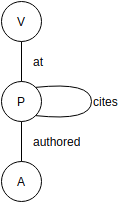
\includegraphics[width=0.25\textwidth]{images/jm2017_undiced_pub_view.drawio.png}
    \vspace{-20pt}
    \caption{Set-theoretic publication model of papers (P), venues (V), and 
authors (A) (adapted from~\cite{JM2017})}
    \label{fig:jm2017_induced_pub_model}
    
\end{wrapfigure}


% \begin{figure}[H]
% \centering
% 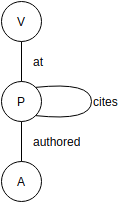
\includegraphics[width=3cm]{images/jm2017_undiced_pub_view.drawio.png}
% \caption{Set-theoretic publication model of papers (P), venues (V), and 
% authors (A) (adapted from~\cite{JM2017})}
% \label{fig:jm2017_induced_pub_model}
% \end{figure}
% In this figure, the V stands for venue, P for publication and A for author. 
% Based on this model, research is conducted to identify if interesting authors 
% can be identified based on metrics derived from this model. One such research 
% is the work of Tielenburg~\cite{TEJ2017}. Unfortunately, the results where not 
% sufficient to provide a solid framework to detect interesting authors.

% ==============================================================================

Whereas the Jonker and Mauw only modelled the author as a role in the process, 
Bj\"ork and Hedlund mention the publisher, editor and reviewer as well. 
We consider the author from Jonker and Mauw the same as the researcher from 
Bj\"ork and Hedlund. In this research, we ignore the publisher. Although the 
publisher is responsible in the end and sets the regulations and constraints for 
editors to work within, the actual work is delegated to editors.

% Hier moet nog iets meer. Bijvoorbeeld: https://www.councilscienceeditors.org/resource-library/editorial-policies/white-paper-on-publication-ethics/2-1-editor-roles-and-responsibilities/


% Unfortunately, Bjork and Hedmung lacks the opportunity to describe the process. However, we can get some textual information from Cormode from his work as an associate editor~\cite{C2013}.

% Cormode also focusses on the journal publication. We will gather the roles and responsibilities from his article and use this to complete our perspective.
% % ==============================================================================
% \paragraph{Editorial Board} Cormode describes that the structure can vary depending per journal. In most cases, generic structure for a journal is that there is a editorial board. This board consist of the Editor-in-Chief and multiple Associate Editors. The main role of this board is to determine which papers to accept.
% % ==============================================================================
% \paragraph{Editor-in-chief} This role decides which papers to include. The information to make this decision comes from the Associate Editor. This role receives the actual papers and delegate the work to associate editors.

% % ==============================================================================
% \paragraph{What about the author}
% Cormode also describes certain roles in the process~\cite{C2013}. In our case,
% the suggestions he makes for an publishing author are important: 1) Suggest
% suitable Associate Editor and 2) Suggest suitable Reviewer. If the
% editor-in-chief and associate editor make use of this suggestion, the author can gain power in the judgement of his own work.



% \outline{
% \begin{itemize}
%     \item Reviews
%     \item vaak meerdere
%     \item daarom minder risico op fraude???
%     \item ali \& watson bekijken
% \end{itemize}
% }

% ==============================================================================
% \section{Extending the model}
Extending the model of Jonker and Mauw with the description of Cormode
\cite{C2013} results
in a model that incorporates the most important roles with influence on the 
judgement of the work of an author. We 
ignore roles like the editorial assistance and subeditor, because these roles 
does not seem to have influence on the judgement of a manuscript. 

In 
Figure~\ref{fig:structure_journal} we provide an overview of the entities and 
roles from Jonker and Mauw combined with the information from Cormode which 
answers the roles involved and their dependencies.

The red rectangles are objects and the green circles are roles.
As objects we have a venue which contains papers. Multiple roles are related to
these objects.
% We define the following sets:
% \begin{itemize}
%     \item Authors: $A(p) = \{h \in H \mid \authors(p, h)\}$
%     \item Reviewers: $R(p) = \{h \in H \mid \reviews(p, h)\}$
% \end{itemize}


% ==============================================================================

% \begin{figure}[H]
%   \begin{center}
%   \small
%         \begin{tikzpicture}[
%             auto,node distance=2cm,thick,
%             rolenode/.style={circle, draw=green!60, fill=green!5, very thick, minimum size=1.05cm},
%             thingnode/.style={rectangle, draw=red!60, fill=red!5, very thick, minimum size=1.05cm},
%             ]
%             % Nodes
%             \node[rolenode] (eic) {EiC};
%             \node[rolenode] (ae) [below=of eic] {AE};
%             \node[rolenode] (reviewer) [below=of ae] {R};
            
%             \node[thingnode] (venue) [left=of eic] {V};
%             \node[thingnode] (publication) [left=of reviewer] {P};
%             \node[rolenode] (author) [below=of publication] {A};
            
%             % Lines
%             \draw[->] (publication) -- node [text width=2.5cm,midway,above,sloped] {published at} (venue);
%             \draw[->] (eic) -- node [midway,above,sloped] {responsible for} (venue);
%             \draw[->] (eic) -- node [midway,above,sloped] {accept / reject / receives} (publication);
%             \draw[->] (reviewer) -- node [text width=2.5cm,midway,above,align=center] {reviews} (publication);
%             \draw[->] (author) -- node [midway,above,sloped] {authors} (publication);
%             \draw[->, transform canvas={xshift=2pt}] (eic) -- node [midway,above,sloped] {assigns} (ae);
%             \draw[->, transform canvas={xshift=-2pt}] (ae) -- node [midway,above,sloped] {recommendation} (eic);
%             \draw[->, transform canvas={xshift=2pt}] (ae) -- node [midway,above,sloped] {assigns} (reviewer);
%             \draw[->, transform canvas={xshift=-2pt}] (reviewer) -- node [midway,above,sloped] {feedback} (ae);
            
%             \path (publication) edge [loop left] node {cites} (publication);
            
%             % \draw[->] (publication.west) .. controls +(down:7mm) and +(left:5cm) .. (publication.west);
%         \end{tikzpicture}
%   \end{center}
%   \caption{Set-theoretic model of the publication process for collections.}
%   \label{fig:structure_journal}
% \end{figure}

\begin{figure}[H]
\centering
\includegraphics[width=11cm]{images/chp_5/set_theoretic_model_of_pub_process_collections.png}
\caption{Set-theoretic model of the publication process for collections.}
\label{fig:structure_journal}
\end{figure}

It is important to notice that the green circles are roles, not entities. These 
roles are fulfilled by people. This results in one more entity (person) with 
relation to other entities. These relationships can be expressed as the roles 
(e.g. a person is a reviewer for a publication).

% ==============================================================================
\subsection{Conferences}
So far we only focused on the process of journals. But, as mentioned before, 
publishing for a conference is important in the Computer Science domain.

In case of conference publications, the author, publication and its relation to 
the venue stays the same. It can be that this venue becomes more extensive 
because of tracks, but it stays a venue.

An important person for conferences is the Program Committee Member. Eventually
this is again a role of a person related to the venue.

% ==============================================================================
\subsection{Resulting model}
\label{sec:resulting_model}
In the resulting model we choose to abstract the roles away and use one entity 
called person where we define the roles to certain entities in the relationship.
This makes the model far more easy to reason about when a person has multiple 
roles.

The model in Figure~\ref{fig:resulting_model} is a logical model. A physical
model can be designed based on this logical model using design
strategies like Ensemble Modelling (e.g. Data Vault~\cite{linstedt2015building}
or Anchor modelling~\cite{ronnback2010anchor}). Which
modeling principle is being applied is not important. What is important, is that
the physical model address requirements like time-awareness and tracking changes
of entities to create a physical model. E.g. a person is not 'always' 
editor of a venue, this role starts and stops at a certain moment in time.
\begin{figure}[H]
\centering
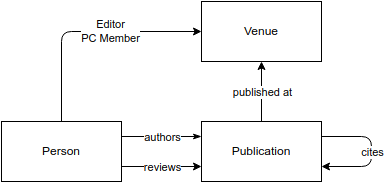
\includegraphics[width=9cm]{images/set_model.png}
\caption{Set model which covers necessary entities and relationships}
\label{fig:resulting_model}
\end{figure}

% ------------------------------------------------------------------------------
\subsection{Example: Publications cites publications in same venue}
\label{interesting_case:publications_cites_publications_in_same_venue}
In this part we will go through a situation to describe the process of analysing
a situation which can be an attack on the publication process and plot this on the
resulting datamodel from the previous section. The chance this 
particular situation occurs is not very high. The reason is that there is a good
enough safety net to catch this situations provided by Thomson Reuters\footnote{\url{https://clarivate.com/webofsciencegroup/solutions/journal-citation-reports}}, 
institute that 
calculates the Journal Impact Score. Besides, in our research we are looking for
interesting people. Because this description method of an interesting case is
used later in this thesis, description of the steps taken are added. 

\textit{First we describe the situation and provide a model of instances that 
are involved. This can be a person in a certain role, venues, publication etc}.

Having publications citing publications from a certain venue, increases the 
journal impact factor.

Figure~\ref{fig:cpsv} is a model of this situation; a venue (v1) that
contains a publication (p1) which has a citation (c1) to a publication (p2) in
the same venue.

\begin{figure}[H]
\centering
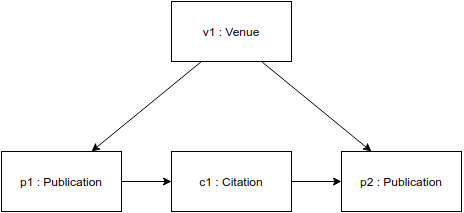
\includegraphics[width=9cm]{images/cited_publications_same_journal.drawio.png}
\caption{Instance model of citation of publication in the same venue}
\label{fig:cpsv}
\end{figure}

% ------------------------------------------------------------------------------
\paragraph{Attack}
\textit{We describe when (this is not always the case, see 'Beneign 
alternatives') and how this situation is an attack.} 

It is not unusual that 
publications in a journal cite publications from the same venue. However, as
with most attacks, when this occurs much more 
compared with other venues and the 'inner venue'-citation rate is significant higher, it becomes 
interesting. This may indicate that this is a conscientious action to increase
the Journal Impact Score, and this can be considered an attack.

\paragraph{Model impact}
\textit{In this part we describe how this situation impacts the publication 
model. What does in- or decrease and how does this impacts the 'score' 
of the attacker.}
The impact on the publication model is that the number of citations to 
publications in the same venue raises. Therefore, the impact score of a journal
raises. 

\paragraph{Beneign alternatives}
\textit{In this part we describe how this situation can occur, while not being
an attack.} 

If a certain venue is that specialised in a certain topic, the 
situation where a publications cites other publications in that venue can occur.



% \section{Main source}


% \subsection{Data acquisition}


% \outline{
% % \begin{itemize}
% %     \item Question to answer: Which data do we need and how can we get it?
% %     \item om te weten welke data we nodig hebben kijken we naar het publicatie process -> beschreven in voorgaand hoofdstuk
% %     \item vervolgens kijken we naar de data die beschikbaar is in de publiek beschikbare databronnen
% %     \item mismatch
% %     \begin{itemize}
% %         \item welke informatie missen we
% %         \item hoe kunnen we hier aan komen
% %     \end{itemize}
% %     \item ophalen van mismatch
% % \end{itemize}

% }

% ==============================================================================
\section{Public available datasets}
In this section we will explore some publicly available datasets with the focus 
on Computer Science which can be used to fill the model from 
Section~\ref{sec:resulting_model}. Because of the necessary ability to integrate 
datasets, we will judge these sets on integrability and completeness.

As a guideline, we will use Figure~\ref{fig:dataflow_jm2017_a}. Our main target
is to create a publication view based on the data sources which are represented
in the figure as `raw data'.
\begin{figure}[H]
    \centering
    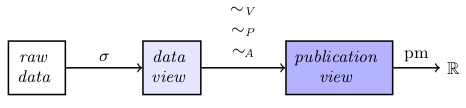
\includegraphics[width=10cm]{images/data_to_publication_metrics_jm2017.png}
    \caption{Data flow (\cite{JM2017})}
    \label{fig:dataflow_jm2017_a}
\end{figure}

The sigma-sign represents the filter on the set. For now, this filter sets the 
focus on the Computer Science area. Later on, this filter can be more 
strict, depending on the case study.

A known datasource for Computer Science in DBLP. We can use this dataset as base.
For other research areas, other datasources should be taken (e.g. for 
biomedical research, one can use PubMed).

% \begin{itemize}
%     \item Publicly available sources are limited in available data. Most datasets provides information on who wrote what and sometimes which article refers what. This provides a good insight and based on these datasets a lot of research is already conducted.
%     \item However, we think these datasets miss actors on the publication process that are in a position with enough power to influence the publication process.
%     \item Data about these people involved in the publication process are not structured available to use in analysis. The information is provided in front matters and masthead documents. Because of the nature of these documents, mostly PDF's, we consider this as unstructured data.
%     \item We are somehow surprised of the lack of structured data availability about these people, because of their power and influence.
%     \item Our focus in this chapter is to incorporate this less structured available data into publicly available data about the publication process to get a dataset which provides a more complete view of the publication process.
%     \item Our research focus on information technology so our start point to gather these people is to use the most prominent conferences and journals. As source for this data we use the core ranking.
% \end{itemize}

% \outline{
% \begin{itemize}
%     \item Model wat in dblp, aminer en in HJ staat
%     \item Model publicatieprocess
%     \item Sluit niet aan
%     \item meer rollen -> niet in publieke datasets
%     \item Most public available datasources for the publicationprocess contain information about the author and what the author publishes. Sometimes (but not all, or incomplete) these datasets also contain references.
%     \item The model of these datasets are visualized by the publication process of Jonker and Mauw.
%     \item Examples of these datasets are DBLP and Aminer.
% \end{itemize}
% }


% ==============================================================================
\subsection{DBLP}
DBLP is a dataset with bibliographic information in the computer science 
discipline which can be downloaded in XML format. In 
Figure~\ref{fig:set_model_dblp} we show which elements of the set are 
covered by DBLP.

\begin{figure}[H]
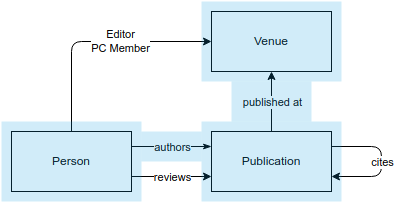
\includegraphics[width=9cm]{images/set_model_dblp.png}
\centering
\caption{Set model DBLP}
\label{fig:set_model_dblp}
\end{figure}

% \outline{
% \begin{itemize}
%     \item Structure of delivery
%     \item Processing
%     \begin{itemize}
%         \item convert XML to relational tables
%         \item Every bibliographic type in separate table
%         \item Assign unique id
%         \item Make separate table for elements with id of bibliographic record
%         \item Attributes of elements are columns in table
%         \item Add metadata to all data entries
%     \end{itemize}
%     \item Result
%     \begin{itemize}
%         \item 35 tables
%         \item overzicht van tabellen en relaties
%     \end{itemize}
% \end{itemize}    
% }

Unfortunate DBLP misses some important information to be complete; the dataset
does not contain references, editors, PC members and reviewers. For 
references, other sources can be addressed: Aminer, OpenCitations or Google 
Scholar.

% ==============================================================================
\subsection{Aminer}
Aminer positions itself as an AI for academic publications~\cite{Tang:08KDD}. 
One dataset they provide is the 
'Citation Network Dataset'. This dataset combines data mainly from DBLP, ACM (a 
publisher) and MAG (Microsoft Academic Graph). Becauses it uses DBLP as a 
source, it is interesting to 
investigate if we can use this for filling the gap of the citations shown in 
Figure~\ref{fig:set_model_dblp}.
In Figure~\ref{fig:set_model_aminer} we presented which entities and roles
from our ideal data model this dataset contains. Although this set contains data
from these entities, the attributes are limited; the main purpose of this set is
citations.
\begin{figure}[H]
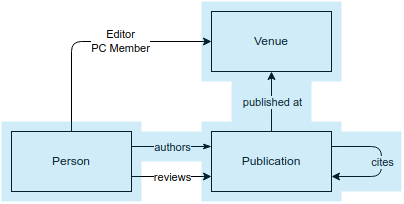
\includegraphics[width=9cm]{images/set_model_aminer.png}
\centering
\caption{Set model Aminer}
\label{fig:set_model_aminer}
\end{figure}


\subsection{OpenCitation} 
OpenCitation is a \doi{} based reference dataset. This means, the cited and citing 
articles are referred to by a \doi{}. 
The dataset from opencitation can be downloaded, or questioned by an \api{} request. 

From the publication entity it only contains the \doi{}.


\subsection{Google Scholar}
\label{subsec:google_scholar}
Google Scholar also contains the references from and to articles. This data is 
only available online. Some software packages exists that support scraping this
information. However, experiments from the research preparation phase concluded
that this was not a feasible solution because of the amount of captcha's when
trying to scrape the site. The acquisition of this data is not practical.

\subsection{Conclusion data availability}
\label{subsec:ConclusionsDataAvailablity}
Referring to the ideal model as given in Figure~\ref{fig:resulting_model}, we 
can make a few statements:
\begin{itemize}
    \item The availability of data about publications, venues and authors is 
    good; almost all public sources contains some information about these 
    entities. 
    \item References are available in two public available sources (we ignore 
    Google Scholar for given reasons in Subsection~\ref{subsec:google_scholar}).
    \item Other roles than `author' are not available in public datasets.
\end{itemize}

In the next section we will investigate how these sources can be integrated.

% \section{Deviation publication model and available data}
% As visualised in Figure~\ref{fig:set_model_dblp} and Figure~\ref{fig:set_model_aminer}, both datasets miss some crucial roles.
% Both sources miss the reviewer, editor and PC Member. These roles are crucial in the publication process and are a must-haves in our group-based outlier detection.

% This raises the question where we are able to get this data. Luckily, there are is some data about these roles publicly available, but this is not straight forward. We will come back to this point when we describe the case studies.

% ==============================================================================
\section{Integrability}
\label{sec:data_integrability}
People, articles and venues can be acquired from multiple source. To be able to 
work with these entities, we need to integrate these sources in one model. To 
make this possible, we need to uniquely identify the entities.

Again referring to Figure~\ref{fig:dataflow_jm2017_b}, we can consider this the 
tilde sign.

\begin{figure}[H]
    \centering
    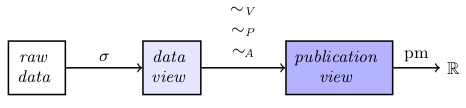
\includegraphics[width=10cm]{images/data_to_publication_metrics_jm2017.png}
    \caption{Data flow (\cite{JM2017})}
    \label{fig:dataflow_jm2017_b}
\end{figure}

In the ideal situation is that entities have an unique identifier which is 
independent of the source. However, in practice it is a bit more complex than 
that.

% ==============================================================================
\subsection{Articles}
The unique key which is used to identity an article is the Digital Object 
Identifier. This field is available in DBLP, Aminer and OpenCitations. Also, the
\doi{} should be unique across all articles. 
Theoretically, combining the sets using the DOI should be possible without much
effort.

However, an analysis of the DBLP data set leaves us with a few DOI's which refer
to multiple articles. The number of articles this occurs, is very low
(approximately 20 articles; a manual override is a possibility). Also, DBLP 
has a lot of documents where the DOI is unknown; so data completeness 
is an issue here. 

\subsubsection{DOI Availability}
\label{subsec:data_doi_availability}
\textbf{DBLP} contains additional information about an entry in an ee tag. These contain 
links to doi.org, wikidata, etc. Sometimes an article has multiple doi.org links; 
this seems mostly the case with the publisher ACM. Although the links are 
different, they redirect to the same page at ACM.
For articles the following count of DOI's is available.
\begin{center}
    \begin{tabular}{ rr }
        \toprule
        \# of DOI & \# of articles \\
        \midrule
        0 & 1,051,229 \\
        1 & 4,626,193 \\
        2 & 22,396 \\
        $\geq$ 3 & 1,202 \\
        \bottomrule
    \end{tabular}
\end{center}

Concluding; most articles do have a \doi{}; approximately 78\% has one or multiple 
\doi{}'s.

% ==============================================================================
\textbf{Aminer} provides one \doi{} field for an article. Also not all DOI's are 
available. For the 4894081 articles in Aminer, 3920939 has a \doi{} (approximally 
80\%). However, the \doi{}'s provided in the dataset are not unique: 3316 DOI's are 
used to identify multiple articles. A quick investigation learned us that Aminer 
sometimes uses a \doi{} to refer to a journal instead of an article. Another 
finding with a quick analysis in the case of \doi{}'s, is that multiple articles
are represented multiple times in the dataset; the article dataset is not 
unique. This raises some doubt about the quality of the dataset of Aminer.

\subsubsection{Alternative key}
Because the \doi{} is not a useful key across all sources to integrate data 
because of availability and uniqueness, alternative fields that make a good 
candidate to serve as key are looked in to. 
A combination of title, authors, year and journal makes a good candidate.
% ==============================================================================

The title and how sources save this title may differ. 
Sometimes the sources uses other characters. For example, \dblp{} uses an HTML
tags to specify characters in the title, e.g. see 
Listing~\ref{lst:DblpTitle}. This in combination 
with specific symbols (e.g. Greek delta-sign) which are expressed differently 
depending on the source, makes joining sets on titles with these signs
cumbersome.

\lstset{language=XML}
\begin{lstlisting}[caption={Example title in \dblp{}},label={lst:DblpTitle}]
<title>Graphs of Bounded Treewidth can be Canonized in AC<sup>1</sup>.</title>
\end{lstlisting}

These problems can be overcome by applying some clean rules before the join. 
Considering a solution for the title exists, still a join on other attributes
needs to be done; the title itself is not unique.
Which raises a next integration problem: people.

% ==============================================================================
\subsection{People}
\label{sec:integrability_people}
In the publication domain an identifier for a person exists, this is called
the Open Researcher and Contributor ID (\orcid{}). This field is (partially) 
available in \dblp{}, but not in Aminer.

Alternative approach to uniquely identify authors is the name. However, this has
multiple issues:
\begin{description}
    \item[Format] A name can be written in multiple formats. E.g. a person is 
    named Alfred Jodocus Kwak; this can be written as `Alfred Kwak', 
    `Alfred J. Kwak', `A. J. Kwak', `A. Kwak' and off course the full name. 
    With names that contain accents on letter, the possibilities increases.
    Also, in some countries it is used to put the family name first.
    \item[Multiple people with same name] The name does not make an author 
    unique. The same name refers to other authors. 
    \item[Other names for the same person] E.g. when Robert is also called Bob.
\end{description}

Both DBLP and Aminer acknowledge this problem. In case of multiple 
people with the same name, DBLP addresses this problem by suffixing the
name with a four digit code\footnote{\url{https://dblp.org/faq/1474704.html}}.
\dblp{} is making progress here, but this is not entirely done yet. 
The format issue and alias issue is covered by \dblp{} by creating a master 
record for the author, see Listing~\ref{lst:DblpAuthorMasterRecord} as an 
example.
Aminer uses an approach which takes the coauthors in to account. It creates
a network of co-authors for a certain author and then calculates a 
probability that this is the same author.
% ==========================================================================
\lstset{language=XML}
\begin{lstlisting}[caption={Example master record (\url{https://dblp.org/faq/1474690.html})},label={lst:DblpAuthorMasterRecord}]
<www key="homepages/r/CJvanRijsbergen">
<author>C. J. van Rijsbergen</author>
<author>Cornelis Joost van Rijsbergen</author>
<author>Keith van Rijsbergen</author>
<title>Home Page</title>
<url>http://www.dcs.gla.ac.uk/~keith/</url>
</www>
\end{lstlisting}

However, an exploratory analysis of the DBLP data makes clear this is not 
flawless; cases exist where the same master record authors one 
article multiple times. After a small investigation it seems that a father 
and son both authored this article (Robert and Bob, same lastname so DBLP 
'chooses' to treat these names as the same person).

But hypothetically, even if DBLP mentions to unique identity authors, 
the match to authors in other datasources is not possible, if these sources 
do not adhere the same method.

% \subsection{Article integration}
% Not only do we need to match the articles of DBLP and Springer LNCS, we also 
% need to incorporate Aminer. Aminer is an enrichment of DBLP in that it adds
% citations. Although DBLP is working to incorporate citations in their dataset,
% this is still work in progress and Aminer has already a lot of that data.

% \begin{figure}[H]
%     \centering
%     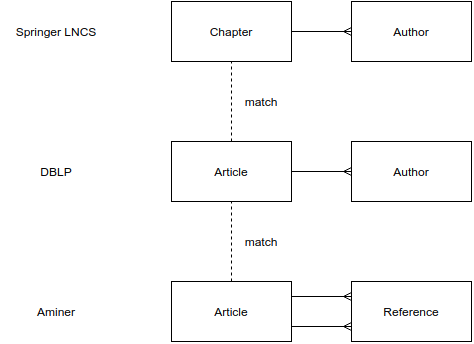
\includegraphics[width=10cm]{images/linking_article_dblp_lncs_aminer.drawio.png}
%     \caption{Matching Springer LNCS, DBLP and Aminer}
%     \label{fig:linking_article_dblp_lncs_aminer}
% \end{figure}


% ==============================================================================
\subsection{Conclusion integrability}
From this section we can draw the following conclusions:
\begin{itemize}
    \item Attributes that could serve as a cross-source key to integrate data 
    (\orcid{}, \doi{}) are not complete enough;
    \item Alternative methods to integrate the data have too many weak spots to
    serve as a sustainable solution;
    \item Therefore, integration of datasets is cumbersome.
\end{itemize}

Combining these statements with the statements from 
Subsection~\ref{subsec:ConclusionsDataAvailablity}, we choose \dblp{} as root 
for the dataset and choose to add additional data depending on the case study.



% Because of the lack of integrability we are unable to fill the citations, 
% although Aminer and OpenCitations can deliver these. 

Therefore, for the case studies a pragmatic approach should be taken; determine 
what data we need to incorporate, what attributes are at our disposal and make 
choices based on that information.

Next step is to actually load the data of \dblp{}.

% ==============================================================================
\section{Processing of DBLP dataset}
The dataset that can be downloaded of DBLP is XML based. For every bibliograpic 
record the file contains a XML element. These record contains elements with 
additional information, e.g. author, title and journal. In 
Listing~\ref{lst:DblpExample} we show one bibliographic record (an article) as 
delivered in the dataset of DBLP.

\lstset{language=XML}
\begin{lstlisting}[caption={DBLP bibliografic record example},label={lst:DblpExample}]
<article mdate="2019-10-25" key="tr/gte/TM-0332-11-90-165" publtype="informal">
<author>Frank Manola</author>
<author>Mark F. Hornick</author>
<author>Alejandro P. Buchmann</author>
<title>Object Data Model Facilities for Multimedia Data Types.</title>
<journal>GTE Laboratories Incorporated</journal>
<volume>TM-0332-11-90-165</volume>
<month>December</month>
<year>1990</year>
<url>db/journals/gtelab/index.html#TM-0332-11-90-165</url>
</article>
\end{lstlisting}

% ==============================================================================
Possible approaches to load this dataset are:
\begin{description}
\item[Option 1: Load all elements to separate tables] This approach splits all 
the data in separate tables; it converts this semi-structured dataset into a 
structured (relational) dataset. The positive points are that we have all data 
(probably also data we do not need, but we do not know that at forehand) and it 
is a process which can be automated. Also, storing the dataset in a 
relational database gives the opportunity to integrate the data with other 
sources. However, this approach leads to a lot of tables, cost storage and 
requires a structure that keeps the referential integrity.
% ==============================================================================
\item[Option 2: Keep it as a file and make software to question the file] We can 
choose to not load the data at all, and create some interfacing to the file to 
be able to read the data. By taking this approach we need to know the model of 
the data at forehand and create software that gives access to the data in the 
file. Also, we are not able to easy query the data, unless we build this 
functionality; functionality which already exists in \mbox{every} other database. 
However, taking this approach does not need to copy the data into another 
structure, which is positive for disk allocation.
% ==============================================================================
\item[Option 3: Split the file in separate XML's and load these in the database] 
Nowadays, databases are able to handle a XML structure as a native datatype. The 
drawback is that, even current relational databases support this task, the 
performance is not optimal. Also querying this data is more complex and slow 
compared when all data is relational stored. Using another type of database is also 
an option (document based). However, for analysis tasks we are going to perform, 
this is not an ideal solution. These document databases are built for 'single' 
requests (e.g. to support an API with predefined requests), and not for 
analysis workloads (e.g. aggregating).
\end{description}
% ==============================================================================
The approach we take is to load all subelements in separate tables (option 1).
The main reason is the possibility for integrating 
this set with other sources. Given the example in Listing~\ref{lst:DblpExample}, 
this results in multiple tables: Article, which is the main object, Author, 
where all authors can be put and separate tables for title, journal, volume, 
month, year and url.
% By extracting these elements in a separate table we can normalise the data.
% We can even go further and normalise everything, which makes it easy to automate the load of data.

% This code part will then 
% \begin{description}
%     \item[All data] By using this approach, we load all the data. We do not need to specify which data we need at forehand, which is a tedious task with a huge XML file (the file is 3,4 GB).
%     \item[Easy to automate] We can automatically see all the attributes in the article element and create tables for the fields.
% \end{description}
% Drawbacks of this approach are:
% \begin{description}
%     \item[A lot of tables] For every element we need to create a table. This can decrease the overview of available data.
%     \item[Storage] Loading all the data comes with a cost in storage.
%     \item[Unnecessary data] All the data means also data we do not need.
%     \item[Relationships] Because the data is being splitted up accross mutliple tables, we need to keep the referential integrity. We need to add identification to all tables to know which article (or other parent object) is belongs to.
% \end{description}



% \begin{itemize}
%     \item Bibliografische records zijn gedefinieerd door een element met subelementen. Deze subelementen bevatten waardes, en geen andere elementen.
    
%     \item 
%     \begin{itemize}
%         \item zie author element in voorbeeld
%         \item moeten manier vinden om hier mee om te gaan
%         \item oplossing is id generereren voor elk 'parent' object.
%         \item dit zijn objecten die direct onder de tag <dblp> vallen.
%     \end{itemize}
   
    
    
%     \item deze objecten aparte tabellen opslaan
%     \item waarbij tabel naam de naam van het attribuut is (bijv. article)
%      \item ander probleem geen zuivere xml: 

% \end{itemize}





% \section{Overcoming the difference}
% \begin{itemize}
%     \item Tielemans vooral gebasseerd op beschikbare data (DBLP)
%     \item Machtsverhoudingen komen niet terug in de publieke datasets
% \end{itemize}
% \subsection{Justification}
% \begin{itemize}
%     \item Overzicht real-life cases (probleem verder beschrijven)
%     \begin{itemize}
%         \item Voorbeeld Vasilakos, citaten uit 2 journals waar hij zelf in zit
%         \item Publicatie lag
%     \end{itemize}
% \end{itemize}

% \subsection{Process and choices}

% ==============================================================================
\section{Advanced data acquisition}
\subsection{From publisher websites}
\subsection{From frontmatter PDFs}
% ==============================================================================

\section{Conclusion}
% Antwoord op welke data is nodig en hoe komen we eraan
In his chapter we defined the model which we need to fill to be able to 
analyse the publication data. Also, we explained how we can fill this model
with publicly available data sources and what elements are missing. From the 
sets we discussed, none of them contains data to load the relation between 
person and venue (the editor and pc member).
% The most
% important conclusion is that relations with a role of power (e.g. editor) in the
% scientific publication process are not present in publicly available datasets.
In the next chapters we will work out three case studies and dive deeper in 
the missing data and how we can acquire this.



% ==============================================================================
\chapter{Implementation}
% ==============================================================================
\section{Scraper implementation}
\todo{
\begin{itemize}
\item VPN vs.~Tor
\item Elsevier JSONs (parsing).
\end{itemize}
}
\section{PDF front matter parsing}
\section{Data integration}

% ==============================================================================
\chapter{Case study 1: Program Committee Members}
\label{chp:case1}
% ==============================================================================
This chapter focuses on the Program Committee Members as group. We will start 
with a motivation why this group is interesting. After this motivation we will
investigate how we can put the dataset together to perform analysis upon. 
We continue with performing some analysis which give (in combination with the 
other case studies) answer to the main question of this study. In the last 
section we will validate the results of the analysis.

\section{Motivation}
The most important motivation to investigate this group, is that this group is 
in a position with great power. In the end, these people decides which articles
(and which authors) get published. Implicit, they decide whose career is going 
to thrive.
This power becomes evident in an experiment conducted on an Artificial
Intelligence conference; the NIPS experiment.


% \begin{itemize}
%     \item PC Members are in a position with power.
%     \begin{itemize}
%         \item Power of this group indicated with NIPS experiment.
%         \item Decision who gets published, implicit who succeeds.
%     \end{itemize}
%     \item Possible to exploit this power.
%     \item PC Members with high impact power are on high impact conferences.
%     \item Thus, we are focussing on top conferences.
%     \item The goal with this case study is to see if we can identity outliers 
%     within a group of PC members.
% \end{itemize}
% \outline{
% \begin{itemize}
%     \item dat je ze krijgt niet interessant
%     \item wel waarom, en hoe goed
% \end{itemize}
% }

\paragraph{The NIPS experiment}
For scientists getting a paper in a conference is important for their career. 
Unfortunately, the NIPS experiments makes clear that reviewing papers for a 
conference is not a deterministic
process\footnote{\url{http://blog.mrtz.org/2014/12/15/the-nips-experiment.html}}.
If a paper gets approved depends on the composition of the 
responsible committee. This means that the committee judging papers for 
conferences has the power to determine whose paper is being accepted and 
therefore whose career is going to thrive.

\paragraph{}
PC Members are in a position where they can exploit this power. Members with
high impact are members on high impact conferences. This reason, we focus on
top conferences. The goal with this case study is to see if we can identity outliers 
within a group of PC members.
An interesting case related to this group is described in the next section.

% ------------------------------------------------------------------------------
\subsection{Interesting case: Work PC member is being cited}
\label{interesting_case:work_member_editorial_board_cited}
% The editorial board can also be the program committee in case of incollections.
When an author becomes a specialist of a certain subject, it is not uncommon 
that this person becomes member of the editorial board or program committee of a 
venue that handles this specific subject.
New publications regarding this subject will likely be published in this venue. 
It is not strange that this publication cites work of the person-of-interest, if 
he is indeed a specialist.
In Figure~\ref{fig:cweb} we present an instance model of this situation. In this 
model, pers1 represents the person-of-interest. We notice the relation of this 
person to the venue (v1) as an editor and to previous work (p2) as an author. A 
new publication (p1) has a citation to the previous work of the 
person-of-interest (c1).

\begin{figure}[H]
\centering
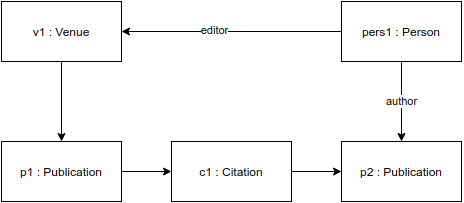
\includegraphics[width=9cm]{images/cite_work_editorial_board.drawio.png}
\caption{Instance model of citation of work of member from editorial board}
\label{fig:cweb}
\end{figure}

% ------------------------------------------------------------------------------
\paragraph{Attack} When this situation is being enforced (malicious intent), it 
becomes attack (e.g. the member says: "cite me, or your work will not be 
published"). The person of interest benefits 
from this situation; he will be cited more, which impacts his metrics (e.g. 
H-Index). The question is now how this enforcement impacts the 
publication model so we are able to detect this. 

% ------------------------------------------------------------------------------
\paragraph{Model impact}
The impact this attack has on the publication model is on the objects Venue, 
Person (with the role editor) and the relationship between. This relationship is 
the fact that a person works for a venue. In this relationship, citations occur; 
while a person works for a venue his work is being cited. In case of an attack; 
we see more citations than usual. The metric we need from this 
relationship is the number of citations: \textit{number\_of\_cites}. But we need 
to take the time into account; if a person works for a venue for a long time 
(multiple incollection or inproceedings are published), it is logic the number 
of cites while being a member is high. Because of this; we also need the number 
of incollection and inproceedings: \textit{number\_of\_issues}.
These metrics can be used for comparison by calculating the 'normal' and the 
deviation of all members. This normal can be calculated over the venue the 
editor is working for, or all venues. This comparison makes it possible to 
identify interesting editors in comparison with his peers.

\begin{figure}[H]
\centering
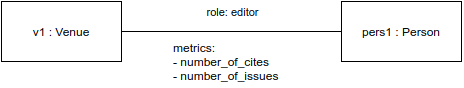
\includegraphics[width=9cm]{images/cite_work_editorial_boardmodel_impact.drawio.png}
\caption{Metrics needed for detection on publication model}
\label{fig:cwebimpact}
\end{figure}

% \begin{itemize}
%     \item Het roept vraagtekens op als gepubliceerd werk referenties bevat van iemand in de editorial board of program committee.
%     \item Dit is niet per se slecht; maar lichtelijk vreemd.
%     \item Als de persoon in de board ook in andere publicaties geciteerd wordt op het moment dat deze persoon in de board zit, wordt de twijfel of dit nog ethisch is groter.
%     \item oog aantal gaat vraagtekens opleveren
%     \item members onderling vergelijken
%     \item kan verschillen per venue
% \end{itemize}

% ------------------------------------------------------------------------------
\paragraph{Beneign alternatives}
The described impact on the publication model can also have other beneign reason 
to occur. The detection strategy is not foolproof. We need to take into account 
that a person is such an excellent contributor, it is logical he is being cited
far more that his peers.

% ==============================================================================
\section{Data acquisition}
% ==============================================================================
In this section we will elaborate which data we need and how we get that data.
The flow from conference to proceedings is shown in
Figure~\ref{fig:data_integration_core_dblp_api}. In the next subsections we 
describe the process steps and datasets of this flow in more detail.

% \begin{wrapfigure}{r}{0.55\textwidth}
%     \centering
%     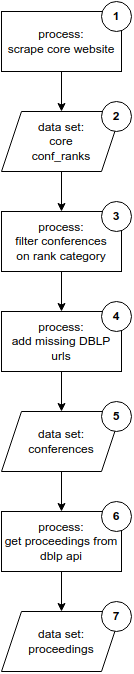
\includegraphics[width=0.40\textwidth]{images/data_integration/core_dblp_api.png}
%     \caption{Gathering proceedings. The parallelogram are 
%     (intermediate) datasets and the rectangles are process steps.}
%     \label{fig:data_integration_core_dblp_api}
% \end{wrapfigure}

\begin{figure}[H]
    \centering
    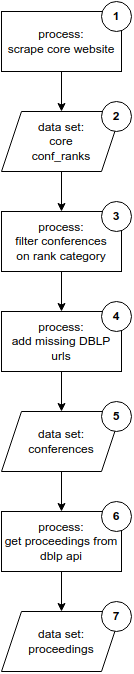
\includegraphics[width=3cm]{images/data_integration/core_dblp_api.png}
    \caption{Gathering proceedings. The parallelogram are 
    (intermediate) datasets and the rectangles are process steps.}
    \label{fig:data_integration_core_dblp_api}
\end{figure}

% ==============================================================================
\subsection{Top conferences}
The focus of this case study is people on a position with influence.
People with influence can be found at top conferences and journals.
Therefore, the primary selection criteria are top conferences and journals.
Considering the dataflow in Figure~\ref{fig:dataflow_jm2017_2}, this is the 
sigma-sign.

\begin{figure}[H]
    \centering
    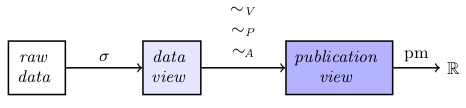
\includegraphics[width=10cm]{images/data_to_publication_metrics_jm2017.png}
    \caption{Data flow (\cite{JM2017})}
    \label{fig:dataflow_jm2017_2}
\end{figure}

For our study, which focuses on computer science, we get the top conferences 
and journals from The Computing Research and Education Association of 
Australasia (core)\footnote{\url{https://www.core.edu.au/}}.

% Not all sources need to be integrated:
% \begin{description}
%     \item[CORE] is used to filter the conferences on score. This source
%     does not contain data that has to be integrated.
%     \item[\dblp{} \api{}] is used to get the proceedings of the conferences. Although 
%     integration of this \api{} source is not needed, we will integrate with 
%     the bulk data from \dblp{}.
% \end{description}

The CORE website provides an export functionality for acquiring data. However, 
for integration purposes, this is not sufficient; the export misses the link to 
the DBLP conference, which is available on their website. For that reason, we 
built a webscraper which is able to get the necessary information for our case 
study (tool: core\_scraper) instead of using the download functionality
(Figure~\ref{fig:data_integration_core_dblp_api}: \textbf{No. 1}, output is 
dataset in \textbf{No. 2}).

Core scores conferences with the following
ranking\footnote{\url{https://www.core.edu.au/conference-portal}}:
\begin{description}
    \item[A*] Flagship conference
    \item[A] Excellent conference
    \item[B] Good to very good conference
    \item[C] Other ranked conferences with minimum standards
\end{description}
Besides these three, they also have 'Australasian', 'Unranked', 'National', and 
'Regional', which is not of interest for our purpose.

Based on their ranking, we select the conferences and journals for our 
research with a ranking of B or higher 
(Figure~\ref{fig:data_integration_core_dblp_api}: \textbf{No. 3}).

The dataset misses 17 DBLP links which we added by hand 
(Figure~\ref{fig:data_integration_core_dblp_api}: \textbf{No. 4}).

The end result is a dataset which contains high-rated conferences with the
DBLP link (Figure~\ref{fig:data_integration_core_dblp_api}: \textbf{No. 5}).

% ==============================================================================
\subsection{Proceedings}
With the selection criteria in place, we can get the proceedings of the 
conferences from DBLP. DBLP provides the option to download the complete data 
dump from their website (described in Chapter~\ref{chp:data}). 
Unfortunately, conferences are not part of this dump. But, with the API of DBLP
we are able to get the proceedings based on the searchterm from the url of core.
We built a tool to load this data from the API in the database, \textbf{No. 6}.
The input for this tool is the dataset shown in 
Figure~\ref{fig:data_integration_core_dblp_api}: \textbf{No. 5}.

The output is a dataset containing the proceedings for the conferences we acquired
from Core (\textbf{No. 7}).

Looking at the publishers of the proceedings we see the following publisher with 
more than 1,000 proceedings:
\begin{table}[h]
    \caption{Publishers with $>$1,000 proceedings}
    \begin{tabular}{ lr }
        \toprule
        Publisher & \#proceedings \\
        \midrule
        Springer              & 4,751 \\
        ACM                   & 4,115 \\
        IEEE Computer Society & 2,422 \\
        IEEE                  & 1,210 \\
        \bottomrule
    \end{tabular}
    \label{tbl:publisher-proceeding-count}
\end{table}
For this case study we want to use the biggest source, which is Springer. 
Springer publishes their proceedings under the Lecture 
Notes of Computer Science (LNCS). The resulting set contains 4,467 unique 
proceedings (the DBLP API search function sometimes returns double results).

% ==============================================================================
\subsection{Acquisition of the PC Members}
On the site of a LNCS proceeding, a front matter document is available for
download. A front matter document contains information about the proceeding,
including people involved in that specific conference; e.g. steering committee,
reviewers and, important for our case, the PC members.

The data acquired from the DBLP API contains the DOI link to 
the proceeding on LNCS (for 1 document this misses, we added it manually). 
With this anchor we can start acquiring the necessary data, including the 
download link to the front matter document.

% ==============================================================================
\subsection{Proceeding information, articles and authors}
\label{subsec:springer_website}
To get the data from \lncs{} we built a webscraper. As input it 
takes the \doi{} links from the \dblp{} \api{} and the output is a dataset with books 
(proceedings), chapters (article), editors and authors and their affiliation. 
See Figure~\ref{fig:lncs_scraper_datamodel} for a graphic representation of the 
entities and their relations.

\begin{figure}[H]
    \centering
    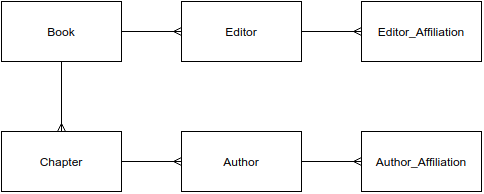
\includegraphics[width=12cm]{images/lncs_scraper_datamodel.drawio.png}
    \caption{Datamodel of the output of the \lncs{} scraper}
    \label{fig:lncs_scraper_datamodel}
\end{figure}

The reason we also extracted the chapters is get the relation between a book and
the articles it contains. To keep our main goal clear: we need to get the people
involved, so while we are scraping the articles, we can scrape the authors just 
as well.

The most important entities we gather from \lncs{} are the books (proceedings), 
chapter (articles) and authors. The editors and their affiliation are not 
important for this case study. 

All chapters we scraped contains a \doi{} as attribute. 
By scraping the books we also get the link to the front matter PDF which can be 
used to download the front matter.

% ==============================================================================
\subsection{PC Members}
We created a simple scraper to download all the front matter from the URL's 
acquired from the previous step. An important step is to convert this collection
of PDF files into information. Because of the effort and size of this step in
the process, we dedicated Chapter~\ref{chp:front_matter_parsing} on this 
step.

In Figure~\ref{fig:flow_proceedings_dataset} we show the flow from the proceedings
to the PC Members.

\begin{figure}[H]
    \centering
    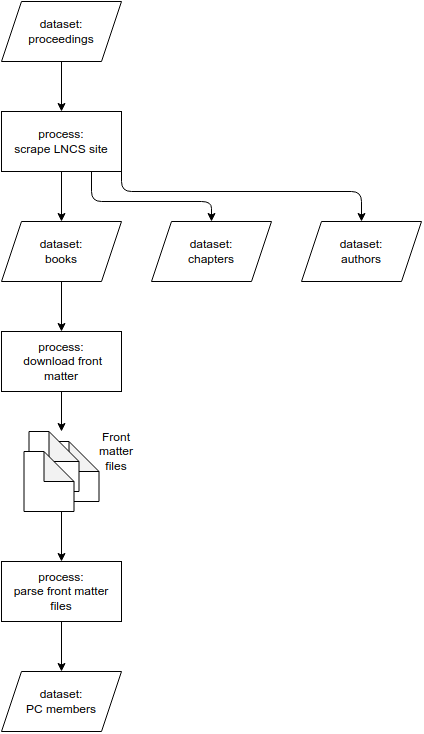
\includegraphics[width=8cm]{images/data_integration/lncs.png}
    \caption{Process \lncs{} data. The parallelogram are (intermediate) datasets 
    and the rectangles are process steps}
    \label{fig:flow_proceedings_dataset}
\end{figure}



% ==============================================================================
\section{Data integration}
In this section we explain how we integrate the data we collected from the
previous section. 

\subsection{Dataset definition}
For this case study we want two datasets.

% ==============================================================================
\subsubsection{Dataset: Published articles}
\label{subsubsec:dataset_published_articles}
This dataset contains information regarding publications members have published 
in their own proceeding. For this dataset we use two sources:
\begin{description}
    \item[Members] Our focus are the members from the proceedings, so the design of the dataset
    should start here. The pragmatic choice we made by using this set, is to only
    take validated data from the front matter documents; see 
    Section~\ref{sec:front_matter_validation}.
    \item[Authors publications] From these members we need to get the articles they wrote. We can use two sources
    for this information: \dblp{} and the data acquired from the Springer website.
    Because the memberset contains the proceeding the member belongs to, and the
    dataset from Springer also contains this proceeding where the article belongs to, 
    we choose to use this dataset.
\end{description}

In Figure~\ref{fig:members_integration_publish} the formalising of the dataset
is shown.

\begin{figure}[H]
    \centering
    \includegraphics[width=11cm]{images/data_integration/members/members_integration_publish.png}
    \caption{Formalising the publishing dataset}
    \label{fig:members_integration_publish}
\end{figure}

The Springer website part (left) is also described in 
Subsection~\ref{subsec:springer_website}. The interested entities from this set
are book (the proceeding) and author. To define the relationship which authors 
publishes in which proceeding, we use the chapter entity.

The front matter part (right) is the result after applying a filter to use 
validated data. 

The relationship between the two sources are based on `\dblp{} key' and `name'. 
The \dblp{} key is the identification from \dblp{} for a certain proceeding.
Because we use \dblp{} as source for gathering the proceedings from the Springer
website we have the key given by \dblp{}. Second, because the Springer website
data is used to download the front matter documents, we can pass this \dblp{}
key to the members.
By taking this approach, we make the \dblp{} key the cross source key for 
identifying a proceeding.

The relationship on the `name' is to match the name of the member with the name
of the author. We use an optimistic approach here by applying a join on the raw 
name; an unmatched name is accepted. As a recap; our purpose is to prove
that a group base approach can help identifying egregious people, we are not 
focusing on creating a foolproof end-to-end solution.
% ==============================================================================

\subsubsection{Dataset: Citation of members}

The sources we integrate for this dataset are:
\begin{itemize}
    \item \dblp{} (Referred articles, authors)
    \item OpenCitation (Citations)
    \item \lncs{} website (Articles, authors)
    \item Front Matter (PC Members)
\end{itemize}

In Figure~\ref{fig:members_integration_citation} we show the sources and their 
relationships to create this dataset.
\begin{figure}[H]
    \centering
    \includegraphics[width=16cm]{images/data_integration/members/members_integration_citation.png}
    \caption{Formalising the citing dataset}
    \label{fig:members_integration_citation}
\end{figure}

\begin{description}
    \item[Members] Also in this dataset, the focus is on the members.
    \item[Articles] The Front Matter and Springer website are joined together 
    just as with the previous dataset, on \dblp{} key. From this proceeded we
    can get the chapters (articles) involved.
    \item[Citations] Because we want to know which authors are being cited in 
    a proceeding, we need the citations. 
    For citations we described two sources in Chapter~\ref{chp:data} which may
    be 
    sufficient. The first is Aminer, which is a dataset that has the articles, 
    references and authors. The second is OpenCitations. Opencitation is \doi{}
    based and we have all the \doi{}'s from 
    the chapters from the Springer website. Because of this, we choose to use 
    OpenCitation as a source for references.
    The dataset from OpenCitation is a download, but very large. For this reason
    we choose to filter the data at loading, so we only load the references from
    articles in \lncs{}.
    \item[Referred articles] The referred articles we get from the \dblp{} dump.
    We could have used Aminer for this, but because the way \dblp{}  handles 
    the names of the author, we choose \dblp{} .
    \item[Cited authors] in the \dblp{} set, we can get the authors of the referred
    articles. With this cited authors we can go back to the members.
\end{description}
% ==============================================================================
For laying the relationships, we use an optimistic approach:
\begin{itemize}
    \item We link the member name to the author name in \dblp{} without additional 
    logic. However, because we use \dblp{} we match against possibly multiple names
    of the author.
    \item Because we use OpenCitation, we only refer to articles in \dblp{} which 
    contain a \doi{}. Another consequence is that we rely on the completeness of
    OpenCitation, but this is an issue with every source we use.
\end{itemize}

\subsubsection{Added value of these datasets}
By having these datasets we can calculate citation and publication metrics for 
members and 
compare them with their peers, which may be in the same proceeding or across 
proceedings, depending on the scope of the peers.


% \subsection{People}
% The author dataset contains all authors for every article. This means, if an 
% author wrote multiple articles, it is multiple times present in this set. For
% our use case, this is not sufficient; we need identify these people as the same 
% person, otherwise collecting metrics for a person is impossible.

% The set we achieved from LNCS conains name, orcid and email. An analysis of this
% set made clear that we got the same name with multiple orcid, or one orcid that 
% refers to more than one person. Concluding: a name does not make a person 
% unique.

% Luckely, DBLP acknowledges this problem. Although they do not yet have all 
% authors unique, they are working on this problem and provide a way to get the 
% unique persons already identified.

% DBLP has the relation between author and article, so to get the `correct' author
% of an article, we need to match the articles in DBLP with the chapters in LNCS.


% \subsection{Integration of persons}

% First challenge is to make the authors unique. This comes with the
% second challenge of data quality.

% For example, from springer we scrape get the chapters (inproceedings) and their 
% authors from their site. This authors sometimes comes with an orcid, which 
% should be unique. However, we found situations where an author gets an orcid of
% someone else. This is a data quality issue.
% voorbeeld toevoegen
% Luckely, this does not occur much, and for the few it occurs we can easily 
% create a manual file to override this. Of course with caution; if two orcid 
% have the same name, we can not override this; some authors have the same name.
% On the other hand, if one orcid refers to a totally different name, we can.

% Seconds challenge is that a name does not make an author unique. The same name
% refers to other authors. Luckely, DBLP addresses this problem by suffixing the
% name with a four digit code~\footnote{\url{https://dblp.org/faq/1474704.html}}.
% DBLP is making progress here, but this is not entirely done yet. But even if
% they mention to unique identity authors, the match to authors in other 
% datasources (like Aminer and Springer) is not straightforward. In that case we 
% need to ignore the authors from these sources and make the match by going 
% through the paper (or chapter, as is it is called within LNCS Springer).

% Third challenge is the name. For most authors these sources do not contain an
% orcid or an email address, which means we need to match the authors on name.
% But, in some sources the names are fully written (with or without the 
% middlename), sometimes the middlename only has a initial while the firstname is 
% fully written, and sometimes we only get the initials and lastname.
% DBLP covers this by naming all aliases of a single person.

% Still we do have a problem, because in the end we need to match these authors
% with members we get from the frontmatters of lncs. Within this frontmatters, 
% there is no orcid, email, or a four digit number to match to dblp records; these
% documents or not written with the intention to identify persons.


% ==============================================================================
\section{Analysis}
\label{sec:cs1_analysis}
% \outline{
% \begin{itemize}
%     \item Wat betekent de data?
% \end{itemize}
% }

From the defined datasets we have the following metrics for every member:
\begin{description}
    \item[\#publications] The number of times the member published in the 
    proceeding he was a member of;
    \item[\#citations] The number of times work of the member is cited in the 
    proceeding he was a member of.
\end{description}

In this analysis we focus on citations from Symposium 
on String Processing and Information Retrieval (SPIRE). The dataset contains 
observations of 483 PC members over 17 years (2003 - 2020).
In Figure~\ref{fig:citation_frequency} we show the frequency of citations. We notice
a large number of zero citations, which means that members during an activity 
(being PC member for a certain proceeding) are not being cited.

\begin{figure}[H]
    \centering
    \includegraphics[width=\textwidth]{images/case_study_1/citation_frequency.png}
    \caption{Frequency of citation count}
    \label{fig:citation_frequency}
\end{figure}

In this phase we need to set the threshold for outlier detection. Eventually
this will be a decision made by domain experts of the publication process.
For our purpose and as an example
analysis we decide to place a threshold at 10 citations; every activity with
more than 10 citations is marked as an outlier.

% For outlier detection we followed Tielenburg and used the Tukey method.



% The IQR 
% we used is 10 (which is very high, resulting in certainty of being positive 
% outliers increases).

% \outline{
% tukey method

% The Tukey's outlier detection method is based on the range of all values.
% First the Q2 is determined, which is the median of all values.
% The median of the values of the lower half, is Q1, and the median of the 
% upper half is Q3.



% \begin{itemize}
%     \item Q1 = median van onderste helft
%     \item Q3 = median of upper half
%     \item IQR = Q3 - Q1
%     \item lower fence = Q1 - 1.5 * IQR
%     \item upper fence = Q3 + 1.5 * IQR
% \end{itemize}
% }

In Figure~\ref{fig:analysis_few} we plotted a few PC member activities. 
Every dot is a member for a certain year of the publication.
The X-axis is ordered by member and year. E.g. we see that 
Member A has 3 citations for the 2018. The Y-axis is the number of citations. 
The red dot in the 
top-right indicates as an outlier. By plotting the data this way, we can quickly
see clusters of outliers, which may indicate members that continues have more 
citations than their peers.

\begin{figure}[H]
    \centering
    \includegraphics[width=16cm]{images/case_study_1/analysis_few_members.png}
    \caption{Example of citation data from Symposium on String Processing and 
    Information Retrieval (SPIRE). (Red lines added for clarity)}
    \label{fig:analysis_few}
\end{figure}



In Figure~\ref{fig:analysis_members} we plotted PC member activities for all PC 
members in SPIRE. The red dots are identified as outliers. One can clearly
identify a cluster (circled by a red dotted-line) which is the same PC member
with activities in multiple years (the name is known by the authors).

\begin{figure}[H]
    \centering
    \includegraphics[width=16cm]{images/case_study_1/analysis_total.png}
    \caption{How often each SPIRE PC member (1993-2020) was cited by each SPIRE where they were PC members.}
    \label{fig:analysis_members}
\end{figure}

% \subsection{Yearly analysis}

% Based on Figure~\ref{fig:analysis_few} one can conclude that it became more 
% usual to being cited in later years, because
% the outlier is in 2020. In
% Figure~\ref{fig:trend_cit_year} we plotted the average number of citations per
% year. The trendline is draw in red and we indeed notice a slight increase of
% the average number of citations per year.

% \begin{figure}[H]
%     \centering
%     \includegraphics[width=16cm]{images/case_study_1/trend_year_cit.png}
%     \caption{Average citations per year for SPIRE (trendline in red)}
%     \label{fig:trend_cit_year}
% \end{figure}



% On the Y-axis we plotted the principal component (dimensional reduction method) 
% over these metrics. The higher, the more the member activity deviates from their
% peers.
% The X-axis are the observation ordered by name and year. By applying this order
% we can quickly identify people who are notorious outliers by seeing the red dots
% next to each other.
% In this figure we circled such a cluster; which is the same person across 
% multiple proceedings (the name is known by the authors).


% ==============================================================================
\section{Validation}
% \outline{
% \begin{itemize}
%     \item Werkt je methode
%     \item Aan het eind van ieder hoofdstuk of een eigen hoofdstuk
% \end{itemize}
% }
As validation we invesigate if the outlier found in the analysis is correctly 
idenitified as an outlier. We can look at this from a data acquisition,
integration, and analysis perspective.
\paragraph{Data acquisition}
In Chapter~\ref{chp:front_matter_parsing} we will elaborate further on the 
validation of the data acquisition from the front matter files.

For other sources we regard the datasets as a given. These datasets are 
considered the building blocks for this research (as they are described in 
Chapter~\ref{chp:related_work} (\nameref{chp:related_work}).

For outlier found during analysis we manually verified that the data was 
correctly parsed from the PDF files. This was
indeed the case. We also noticed that this person was also related to other
conferences
for SPIRE, which were not correctly loaded because of a parse error.

The analysis is based on the whole population across all years. Outliers can
differ if we change the scope. We tried to do this, but then the population
we applied outlier detection upon was too small. 

\paragraph{Integration}
We took an optimistic approach in joining the different datasets together 
because of the limitation in the data described in Chapter~\ref{chp:data}. It
is therefore likely we miss some data. The effects of missing data could be:
\begin{itemize}
    \item Unmatched members in the authorset because the names differs;
    \item Too many authors mathed to a member because of the same name (for
    the outlier we found we verfied this was not the case);
    \item Unlinked refered papers because of the lack of DOI of the reffered 
    paper (the papers from LNCS do all have a DOI provided).
\end{itemize}

Despite the above described threads to the validity, we are able to identify 
outliers. Therefore, we can state that data containing members of proceedings 
contribute to possible fraud detection.

% ==============================================================================
\chapter{Front matter parsing}
\label{chp:front_matter_parsing}
% ==============================================================================
There is more to the publication process than is available in public
datasets like DBLP. Examples are PC memberships, editorships, reviewers (who
reviewed which paper), how fast was the review process, etc.

Some of this data is publicly available, but scattered accross websites and 
other mediatypes meant for people to read and understand, but not
machine-readable and therefore integrated in publication data sets.

For example: Elsevier and ACM give timelines of paper revisions for journal
articles; in their LNCS series, Springer typically lists the PC members in the 
front matter.

This data can be useful for identifying outliers.

In this chapter we investigate how to extract PC members from the LNCS front
matter which can be attained from the LNCS website.

        
% \begin{itemize}
%     \item For example: Elsevier and ACM give timelines of paper revisions for journal
%     articles;
%         in their LNCS series, Springer typically lists the PC members in the 
%         front matter.
%     \item This data may be useful for identifying outliers.
%     \item In this chapter, we investigate how to extract both Elsevier and LNCS
%     data and
%         how to integrate them with existing data sources.
%     \item
%     \item People involved in the proceedings are mentioned in the Front Matter.
%     \item Front Matter can be downloaded as PDF.
%     \item PDF are considered unstructured data.
%     \item PDF's are meant to read by humans, not computers. However, currently 
%         we have 4370 Front Matters, which is an unbearable task to copy and 
%         paste the data manual from these PDF's.
%     \item To be able to get the data inside these PDF's, we need to convert the 
%         PDF's to a structured or semi-structured dataset.
% \end{itemize}
% ==============================================================================
\section{Reading a PDF}
LCNS front matter documents are PDF (Portable Document Format) files. The main
purpose
of this file is described by Adobe as to give``\textit{people an easy, reliable
way to present and exchange documents - regardless of the software, hardware, or
operating systems being used by anyone who views the
document}''\footnote{\url{https://www.adobe.com/acrobat/about-adobe-pdf.html}}. 
In other words; focused on layout and intended for humans to read; not for
computers. 

However, currently we have 4370 Front Matters, which is an unbearable task to 
copy and paste the data manually from these PDF's in a more structured format.
Therefore, to be able to get the data inside these PDF's, we need to convert 
the PDF's to a structured or semi-structured dataset.

Mutliple options to read a PDF programmatically exists:
% ==============================================================================
\begin{description}
    \item[Option 1: Convert to HTML] There are multiple tools available to 
        convert PDF
        to HTML format. Further processing can be applied by using HTML
        libraries. Unfortunately, the resulting HTML pages are complex to
        interpret
        because the content of a  tag can contain just one letter. We need to 
        glue these 
        tags together, with taking the location of the tag in consideration
        (how much space is between two letters, is that a space, is that a 
        new column, or an indent in an existing column etc.). We did an 
        experiment to process PDF's this way, but the resulting solution to 
        process one PDF was not able to process another one. The effort to 
        make this a generic solution which can easily be extended was very high 
        in comparison with the result we achieved (high effort, low result).

    \item[Option 2: Convert to plain text] Almost all libraries to read a PDF 
        file 
        support the option to read the file as plain text. Drawback is that
        the lay-out is gone. This lay-out is necessary to get some structure
        (and therefore `meaning' of the text) from the document. Without this
        lay-out we are unable to identify text as a section header, of identify
        columns in the document.
    
    \item[Option 3: Convert to image and extract text] We can use machine 
        learning libraries to get the text from an image. We tried this 
        with Tesseract, but too much information was lost to get the 
        structure of the document. The same issues applied as with the `convert
        to plain text' option.

    \item[Option 4: Use low level library] In another experiment we tried of 
        we were able
        to process the PDF with a more low level library. This give us more
        control of the process. First small experiments with PDFBox were 
        successful also gives is only text without layout. However, because the
        low-level control we have by using this library, we can adjust this to
        out need.
\end{description}

We choose to proceed with option 4, PDFBox, because of the extensibility and
control we have
and, as mentioned before, other solutions were unable to keep the necessary
structure (option 2 and 3) or needed too many adjustments to make it work with
more and other formatted documents (option 1).
% ==============================================================================
\section{A prototype extractor of raw data}
First we need to get the raw data from the PDF's. PDFBox comes with a parser 
out-of-the-box that gives the PDF back as plain-text. As mentioned  before, for
our case this is not sufficient. The problem is within this text all spaces
between words are converted to one space. However, we need to be able to 
identify columns, so we need to keep all spaces.

Luckely, we were not the only one with this problem. 
An open source parser for PDFBox is made available on
Github\footnote{\url{https://github.com/JonathanLink/PDFLayoutTextStripper}} 
that keeps the layout as is. However, this extension still did not have all
properties of the text we need to get the structure of a file; it only keeps the
spaces between words. 
% ==============================================================================
Because this parser is open source, we are able to adapt this parser to our 
needs; we can add additional properties to the text objects we read from the 
PDF. Besides the text with all the spaces in between (to preserve the layout) we
get by using this extension, we also added the size of the font and the layout
(bold identification).
% \begin{itemize}
%     \item FontSize
%     \item FontSizeInPt
%     \item XScale
%     \item IsBold
% \end{itemize}

The end result of this phase is that we have the PDF file as textobjects with 
the properties we need to transform the raw text in information.

% ==============================================================================
\subsection{Building a document tree}
\label{sec:lncs_parser_doc_tree}
By using the properties textsize and bold properties we are able to identify
headers in the document which we need to build an hierarchical structure of the
document. In 
most Front Matters there is an organization header, with subheaders containing 
the role of the people.

To be able to work with the document struture, we parse this hierarchical
structure in a tree datastructure.
The objects we store in this tree are Sections. These contain the 
textlines and the header as title of the section. 
In Figure~\ref{fig:front_matter_organisation_section} a piece of a front matter
with the organisation part is shown. This makes clear that we need properties as
text size and bold identification to identify headers. 

\fbox{
\parbox[H]{\textwidth}{
    \centering
    \includegraphics[width=11cm]{images/front_matter/organisation_sections.PNG}
    \captionof{figure}{Organisation part in a front matter}
    \label{fig:front_matter_organisation_section}
    }
}


In
Listing~\ref{lst:document_tree} a textual representation of a part of
Figure~\ref{fig:front_matter_organisation_section} is shown.
The most important for our purpose is the section called 'Organization' with
the underlaying sections 'Steering Committee', 'General Chairs', 'Program Chair'
and 'Workshop Chairs', as these as the roles of people involved in this
proceeding.

\begin{lstlisting}[
    caption={Representation of the document},
    captionpos=b,
    label={lst:document_tree}
    ]
{"section":{"title":"DocumentRoot","# lines":1}}
- {"section":{"title":"Lecture Notes in Computer Science 7727","# lines":7}}
- - {"section":{"title":"Editorial Board","# lines":32}}
- {"section":{"title":"Kyoung Mu Lee Y asuyuki Matsushita James M. Rehg Zhanyi Hu (Eds.)","# lines":1}}
- {"section":{"title":"Computer V ision - A CCV 2012","# lines":3}}
- - {"section":{"title":"11th Asian Conference on Computer Vision Daejeon, Korea, November 5-9, 2012 Revised Selected Papers, Part IV","# lines":22}}
- - {"section":{"title":"1 3","# lines":19}}
- - - {"section":{"title":"Preface","# lines":77}}
- - - {"section":{"title":"Organization","# lines":8}}
- - - - {"section":{"title":"Steering Committee","# lines":7}}
- - - - {"section":{"title":"General Chairs","# lines":7}}
- - - - {"section":{"title":"Program Chairs","# lines":7}}
- - - - {"section":{"title":"Workshop Chairs","# lines":8}}
\end{lstlisting}

% ==============================================================================
Having this tree, we can easily get the section that contains the organisation
and all sections underneath.
% ==============================================================================
\subsection{Processing a section}
A section is a textpart of the document. In 
Figure~\ref{fig:front_matter_section} an example is shown. In this example, the
role of the member is the title.
\begin{figure}[H]
    \centering
    
\includegraphics[width=12cm]{images/front_matter/section.png}
    \caption{Section in the Front Matter}
    \label{fig:front_matter_section}
\end{figure}
The text in a section with people involved in the proceeding, has a grid
structure. A visual representation of a grid layed on top of 
Figure~\ref{fig:front_matter_section} is shown in 
Figure~\ref{fig:front_matter_section_grid}. 
% ==============================================================================
\begin{figure}[H]
    \centering
    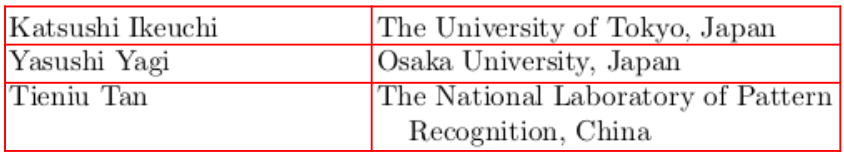
\includegraphics[width=12cm]{images/front_matter/section_table.png}
    \caption{Section in the Front Matter}
    \label{fig:front_matter_section_grid}
\end{figure}
% ==============================================================================
Because of this structure, we use a grid as data structure to put the data from 
the raw lines in to. In Listing~\ref{lst:grid_representation} we show the 
parsed section in a grid representation from the logs files. 
 The challenge in this part is to merge lines into one line.
This process is done in a section-to-grid converter. Separating this
process from the process of building a tree, improves testability.

\begin{lstlisting}[
    caption={Representation of the grid (captured from the application logs)},
    captionpos=b,
    label={lst:grid_representation}
    ]
+------------------+-------------------------------------------------------+
| Katsushi Ikeuchi | The University of Tokyo, Japan                        |
+------------------+-------------------------------------------------------+
| Yasushi Yagi     | Osaka University, Japan                               |
+------------------+-------------------------------------------------------+
| Tieniu Tan       | The National Laboratory of Pattern Recognition, China |
+------------------+-------------------------------------------------------+
\end{lstlisting}

This grid structure gives us some possibilities, e.g. to get statistics of a
column, which we are going to need to choose the correct parser to transform
this text into information.

\subsection{Getting information from a grid}
\label{subsec:front_matter_grid_information}
To get information from a grid we need to parse the text in the grid. For 
this we define a parser interface. The implementation of this interface 
depends on the structure of the grid (e.g. the number of columns) and the 
content (e.g. is it an affiliation or a name).

The properties we acquire from this grid are the following:
\begin{description}
    \item[Number of textparts] The total number of cells that are filled in
        the grid.
    \item[Number of columns] The number of columns that the grid contains.
        Most sections contains two columns, but this is certainly not the 
        case for all sections.
    \item[Affiliation ratio] The ratio of textparts that contain keywords 
        for an affiliation (e.g. "universi"). This is calculated for every 
        column and for odd, even and all rows.
    \item[Comma ratio] Same as affiliation ratio, but for comma's. Can also
        be used to identify affiliations. However, names also contains 
        comma's if the format is lastname, firstname.
\end{description}

In Listing~\ref{lst:front_matter_grid_info} we show some statistics for 
identifying affiliations.

\begin{lstlisting}[caption={Some derived information from the grid},captionpos=b,label={lst:front_matter_grid_info}]
numberOfColumns:	2
affiliationRatios:
	{"columnNumber":0,"rows":"ALL","ratio":0.0}
	{"columnNumber":0,"rows":"ODD","ratio":0.0}
	{"columnNumber":0,"rows":"EVEN","ratio":0.0}
	{"columnNumber":1,"rows":"ALL","ratio":0.6666666666666666}
	{"columnNumber":1,"rows":"ODD","ratio":0.5}
	{"columnNumber":1,"rows":"EVEN","ratio":1.0}
\end{lstlisting}

With this information the program can choose the appropriate implementation
of the parser to
interpret the data correctly and convert the grid into information (members
and affiliations). The resulting objects are shown in
Listing~\ref{lst:front_matter_resulting_information}.
\begin{lstlisting}[
    caption={Resulting information},
    captionpos=b,
    label={lst:front_matter_resulting_information}
]
{
    "name":"Katsushi Ikeuchi",
    "affiliation":"The University of Tokyo, Japan",
    "role":"Steering Committee"
}
{
    "name":"Yasushi Yagi",
    "affiliation":"Osaka University, Japan",
    "role":"Steering Committee"
}
{
    "name":"Tieniu Tan",
    "affiliation":"The National Laboratory of Pattern Recognition, China",
    "role":"Steering Committee"
}
\end{lstlisting}
For example, Listing~\ref{lst:front_matter_grid_info} shows us that 
the ratio of affiliation keywords in the second column (0-based) is 
above a certain threshold and the section consists of two columns, the software 
chooses a Two\_Name\_Affiliation parser which means two columns, first column is a 
name, and the second column is the affiliation.

% ==============================================================================
\section{Data storage}
This process to parse PDF file to usable information results creates the 
following data:
\begin{description}
    \item[Information dataset] Off course, the process outputs the members (name
        and affiliation), the role and the document this information was read 
        from.
    \item[Metadata] Besides this information, the statistics described in 
        Section~\ref{subsec:front_matter_grid_information} and the used parser 
        implementation is also added. We use this to validate the results; see 
        Section~\ref{sec:front_matter_validation}.
    \item[Logging] For every PDF the application parses, a log file is created.
        The purpose is error-detection and the possibility to quickly gather 
        information to extend the software and create the tests; iterative 
        logging-based development.
\end{description}

% \subsection{Database}
% In the database we store three entities: file, section and member. All tables 
% contain at least the following attributes:
% \begin{description}
%     \item[id] Auto generated number.
%     \item[run\_id] The identification of the program run (epoch).
% \end{description}
% In Figure~\ref{fig:lncs_pdf_database} the relationship between the tables are
% shown.
% \begin{figure}[H]
%     \centering
%     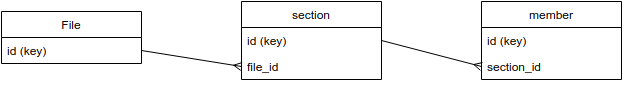
\includegraphics[width=12cm]{images/lncs_pdf_parser_tool.drawio.png}
%     \caption{Relationship between tables}
%     \label{fig:lncs_pdf_database}
% \end{figure}

% \subsubsection{File}
% This table contains information of the file. It can be use to link to previous 
% gathered data. The following attributes are in this table:
% \begin{description}
%     \item[filename] The filename of the pdf to refer to other tables in the 
%         process.
%     \item[status] If the process of the file succeeded or failed.
%     \item[message] If the process failed, how come. 
% \end{description}

% \subsubsection{section}
% This table contains information of the section. The following attributes are in 
% this table:
% \begin{description}
%     \item[title] The title of the section (e.g. Program chair).
%     \item[num\_parts] The number of textparts that are detected in this section.
%     \item[num\_section\_lines] The total number of lines in a section.
%     \item[num\_section\_lines\_non\_empty] The number of lines in a section that
%         are not empty.
%     \item[num\_merges\_lines] The number of lines that are merged in to the 
%         previous line.
%     \item[num\_grid\_rows] The number of rows the grid has.
%     \item[num\_grid\_columns] The nubmber of columns the grid has.
%     \item[all\_values\_contain\_commas] Indicator if all values contain commas.
%     \item[comma\_ratios] A json structure with statistics of comma's in the text.
%     \item[affiliation\_ratios] A json structure with statistics of affiliation 
%         keywords in the text.
%     \item[parser] The parse the program choose to process the section.
% \end{description}

% \subsubsection{Member}
% This table contains eventually the resulting data we are interested in.
% \begin{description}
%     \item[role] The role of the member. This is in most cases the same as the 
%         the title of the section (but, not always). 
%     \item[name] The name as we get from the data, whatever format it is. If we
%         get a separate firstname and lastname from the section, the name is 
%         built based on those values. However, we prefer separate firstname and
%         lastname, because this gives us more options when we need to integrate
%         this data with data from other sources.
%     \item[firstname] If we are able to get separate firstname and lastname of
%         the member, we will store this here. We do tend to interpret names which 
%         contain a comma as <lastname>, <firstname>.
%     \item[lastname] Same as before, but then the lastname :).
%     \item[affiliation] The affiliation of the member. This data is not always
%         available, but we do not tend to use it.
% \end{description}

\subsection{Iterative Logging-based development process}
For every PDF that the program process, it keeps a separate logfile. This gives
us the ability to investigate why the program was unable to process some files 
or sections. Missing parser for example can be detected using this mechanism in
combination with the data in the section table in the database.

For every file the logfile shows the document tree as described in 
Section~\ref{sec:lncs_parser_doc_tree}. 

If sections are found, the logfile shows for every section:
\begin{description}
    \item[Textlines] All the lines that are in this section.
    \item[Grid] The derived grid from the textlines (See
        Listing~\ref{lst:grid_representation}).
    \item[Members] The members that are extracted from the section.
\end{description}
Having this information gives us the possibility to 
investigate in detail why data can not be interpreted and easily build new 
functionality (e.g. new parser implementations) and add unit tests for this 
functionality.

\section{Validation}
\label{sec:front_matter_validation}
Currently 4370 Front Matters are available. How are we able to tell something 
about the quality of the program without manually go through the results?

For every section we gathered some metrics (e.g. number of lines read, number of 
lines merged, chosen parser). With these metrics, depending 
on the parser we can see if the number of extracted members is correct, or close to
correct.

This information can be used to decide if we include the information in the
analysis-datasets.

For example, The parser Two\_Role\_NameAff contains two columns: first with a name
and second with the affiliation. We can measure if the number of resulting 
members is equal to the number of non-empty lines in the section minus the number 
of merged lines. If it is, we can add this data to the analysis-dataset with 
confidence the data is read correctly.

\subsubsection{Current state}
In Figure~\ref{fig:front_matter_result} we show a tree with the file counts.
From the 4370 files we were unable to process 1237 files of which 1119 
because the software was unable to find the organization header. It may be
useful for improvement of the software to tackle this issue first.

Of the correct processed files, 2223 contained interesting sections. These are
section with the role 'program committee'. Of these interesting section, 2711
across 2055 files are validated with the above described method and can be used
during analysis.

\begin{figure}[H]
    \centering
    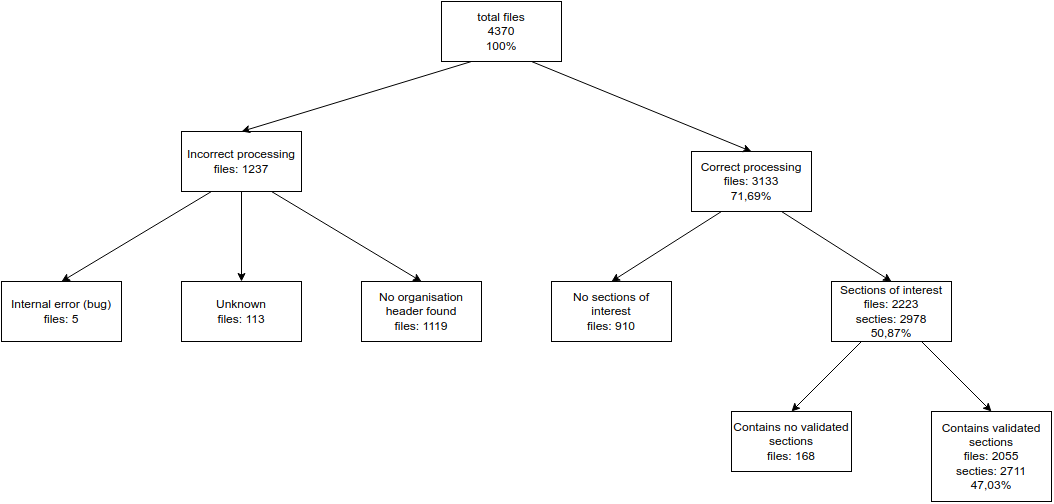
\includegraphics[width=17cm]{images/lncs_front_matter_result.png}
    \caption{Current results}
    \label{fig:front_matter_result}
\end{figure}

% ==============================================================================
\chapter{Case study 2: Journal editors}
\label{chp:case2}
% ==============================================================================
In this chapter we focus on journal editors (editor-in-chief and the associate editors) of 
ACM (Association for Computing Machinery)\footnote{\url{https://dl.acm.org/}}; 
a publisher of journals in the area of computer science.
As with the previous case study, we will start with a motivation and example of
an attack, proceed with the data acquisition and integration and conclude with
an analysis of the data and validation of the analysis.

% ============================================================================
\section{Motivation}
This case study focuses on journal editors, which are in position with great 
power. As previously shown in Figure~\ref{fig:c2013} (repeated in Figure~\ref{fig:c2013_2}), both roles are in 
a position power to make or break a publication and the career of an author.

\begin{figure}[H]
\centering
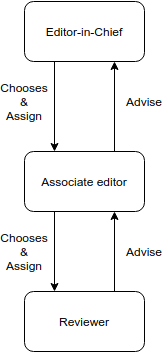
\includegraphics[width=3cm]{images/c2013.drawio.png}
\caption{Roles within the journal process (visual interpretation of description in~\cite{C2013})}
\label{fig:c2013_2}
\end{figure}

\newpage

\subsection{Interesting case: Member of the editorial board is (co-)author}
\label{interesting_case:member_editorial_board_is_coauthor}

In this case, publications in a venue are co-authored by a member of the 
editorial board, which means he is publishing his own work. A questionable 
case in this situation is
\mbox{Griffiths}\footnote{\url{http://deevybee.blogspot.com/2020/07/percent-by-most-prolific-author-score.html}}.
Except for editorial boards, this can also happen for conferences (see 
dataset in Section~\ref{subsubsec:dataset_published_articles} for PC Members).
In Figure~\ref{fig:eia} we present an instance model of this situation.

\begin{wrapfigure}[17]{r}{0.3\textwidth}
    \centering
    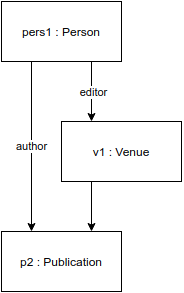
\includegraphics[width=0.3\textwidth]{images/editor_is_author.drawio.png}
    \caption{Instance model of the situation where the editor is \mbox{(co-)author} of the publication}
    \label{fig:eia}
\end{wrapfigure}

% \begin{figure}[H]
% \centering
% 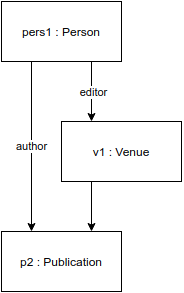
\includegraphics[width=3cm]{images/editor_is_author.drawio.png}
% \caption{Instance model of the situation where the editor is (co-)author of 
% the publication}
% \label{fig:eia}
% \end{figure}


\paragraph{Attack}
We can imagine a situation where the author is being forced to mention the 
person-of-interest as co-author; which is abuse of the power of the editor.

\paragraph{Model impact}
The impact on the publication model is between the person which is 
\mbox{editor} for a 
venue, and the venue itself. 
The number of publications he has in that venue while he works for that 
particular venue 
will increase. For detection we can measure this number of publications:
\textit{number\_of\_publications}. Also with the 
case described in 
Section~\ref{interesting_case:work_member_editorial_board_cited}, we need the 
number of issues.

% ------------------------------------------------------------------------------
\paragraph{Beneign alternatives}
Besides possible ethical questions that can be raised, there may be a valid
reason for someone to publish in the venue he is editing. For example a person
is a 
specialist in his field and works at a venue which specializes in this 
specific subject. He has new work to publish but there is not another venue 
which captures this subject.

\subsection{Case study purpose}
\label{subsec:case2_purpose}
As with all case studies we try prove that adding data not yet integrated in
known datasets and applying a group based outlier 
detection improves fraud detection. In this case, the group
of focus is the editorial board.

We need to compare members of this group. For comparison, we need to identify
the properties that makes them different and may be indicating an attack on the
publication model.

As stated in the interesting case described in 
Section~\ref{interesting_case:member_editorial_board_is_coauthor}, a 
possible attack if being forced 
to add a member of the editorial board as co-author. One possible detection 
method is to see the ratio of unique authors the person-of-interest published
in the journal and outside the journal. If a member publishes inside the journal
with much more unique authors than outside the journal, this may indicate this 
member forces the original author to make him co-author. This case is based
on the assumption that authors have their group of peers they publish most
of the articles with.

In this case study, this is the method we are going to apply.

% ==============================================================================
\section{Data acquisition}
In this case study our focus is the editorial board. Editor-in-chiefs, 
associate-editors and sometimes a list of reviewers (generic, not who reviewed 
what paper) are most of the time available on the publisher website of the 
specific venue. But this has two issues:
% --------------------------------------------------------------------------
\begin{description}
    \item[Machine readability] These roles are not easy machine readable 
    through an interface. It is placed on the website for humans to read. 
    Although good technology exists to acquire data from a website, a minor 
    change to 
    the website can break this method and is therefore not a sustainable
    solution.
% --------------------------------------------------------------------------
    \item[Issue- and time awareness] Only the current editorial board is 
    shown on the publisher website. This may be sufficient for guests of the 
    site, but for extending the datamodel with the editorial board with the 
    purpose of detecting fraud, this is not sufficient. In that case we need 
    to know who was editor for which issue. 
\end{description}
% --------------------------------------------------------------------------
Not everything is lost however; most of the time the previous editorial 
boards are available in so-called mastheads or erditorials of a certain 
issue. These 
mastheads can be downloaded as a PDF (as article of a journal). A formal 
investigation during the research preparation learned us that the format in 
which the editors are presented is not consistent (comparable with the 
front matter of the \lncs{} proceedings).

Theoretically, we can process the data like we did with the \lncs{} Front 
Matter. However, our intention is to prove that an outlier detection 
approach within the group of editorial board members is feasible. As we 
already gathered data from PDF's in Case study 1, we will not repeat this 
technical step (we already show that this is possible) and focus more on 
the functional added value of having editorial board members.

We choose ACM because ACM is a big publisher in the area of computer science
and they present the editorial members in a structured manner on their 
website for all journals. This makes acquiring the data in a automatic 
manner possible.

To gather the editorial board from ACM we first listed some journals where 
we want to get the editorial board from. From this list we scraped the 
editorial board. Figure~\ref{fig:acm_editorial_board} shows a screenshot 
from an editorial board page from ACM.

\begin{figure}[ht]
\centering
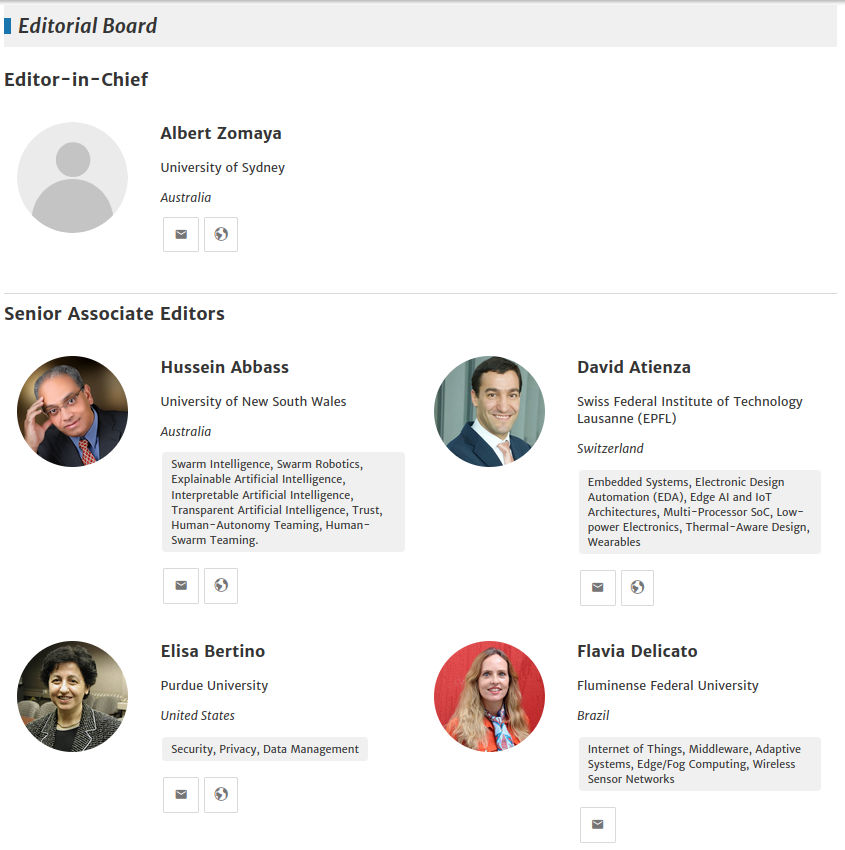
\includegraphics[width=11cm]{images/acm_editorial_board.png}
\caption{Page with editorial board from ACM (\url{https://dl.acm.org/journal/csur/editorial-board})}
\label{fig:acm_editorial_board}
\end{figure}

By building a tool for scraping these sites we can get the role, name, 
affiliation, country and journal name as attributes from this page.

% ==============================================================================
\section{Data integration}
As stated in Section~\ref{subsec:case2_purpose} we want to have the number of
unique co-author a member publishes inside and outside a journal. For this we
need the following entities:
\begin{itemize}
    \item Editors
    \item Articles written by these editors
    \item Co-authors of these articles
    \item The venue where these articles were published
\end{itemize}

We already acquired the editors from the ACM website. The other entities can be 
found in DBLP. 
However, the venue is not straightforward in the dump of DBLP; it is 
encapsulated in the key of an article, see Listing~\ref{lst:dblp_object_key} 
as example.

\lstset{language=XML}
\begin{lstlisting}[caption={Example DBLP key},label={lst:dblp_object_key}]
journals/tomccap/Wang21
\end{lstlisting}

In case of the example, `tomccap' is the abbreviation of the journal. However, 
the name we get from ACM website is only the full name of an journal. In this
case `ACM Transactions on Multimedia Computing, Communications, and
Applications'.
More interestly; this full title is also abreviated as `tomm'; thus the relation
between a journalname and abbreviation is not 1:1.

% ------------------------------------------------------------------------------
\subsubsection{Journal abbreviation lookup}
We need a dataset containing the relationship between the abbreviation and the
full journal name. Two sets were found:
\begin{description}
    \item[Pages at Clarivate] which are the maintainers of Web of Science. 
    Unfortunately, the abbraviations used by DBLP were not found in this set.
    \item[University of British Columbia] also maintains a list. However, the 
    abbreviations they use are different. E.g. in case of the example, their
    abbreviation is `ACM Trans. Multimedia Comput. Commun. Appl.'. DBLP
    also abbreviates journalnames this way, but the 
    abbreviations from this university are not found in DBLP.
\end{description}
The list of journals we want to scrape from ACM is not that large: only 27. So
a manual built dataset is the way we tackle this issue. This is very achievable 
with help of the search functionality on the DBLP site. See 
Figure~\ref{fig:dblp_search_result} as example; the abbreviations used are shown
directly right to the name.
\begin{figure}[H]
\centering
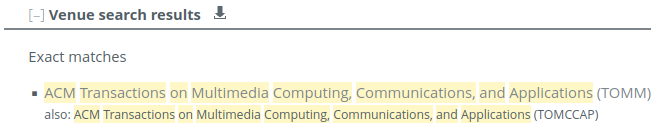
\includegraphics[width=11cm]{images/dblp_search_result.png}
\caption{DBLP search result (\url{https://dblp.org/search?q=ACM+Transactions+on+Multimedia+Computing\%2C+Communications\%2C+and+Applications}).}
\label{fig:dblp_search_result}
\end{figure}
% ------------------------------------------------------------------------------
\subsubsection{Integration model}
With the information from the previous section, we can now build the dataset to
perform our analysis upon. The dataset formulation is shown in 
Figure~\ref{fig:editors_integration_coauthor}. The explanation will follow 
after the image.
\begin{figure}[H]
    \centering
    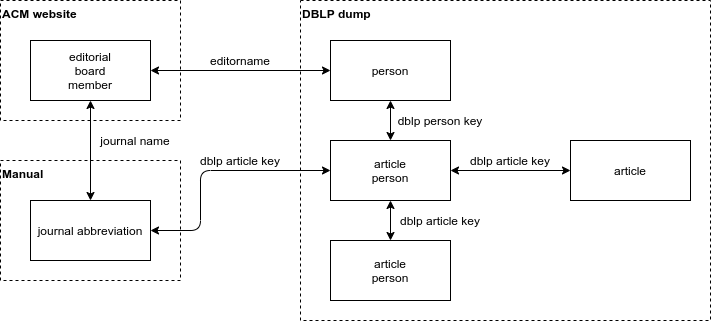
\includegraphics[width=13cm]{images/data_integration/editors/editor_integration_coauthor.png}
    \caption{Formalising the publishing dataset}
    \label{fig:editors_integration_coauthor}
\end{figure}
We start with the editors from the ACM website. By joining the editorname 
to the authorname in DBLP, we can get the unique DBLP name key (because of the 
issues with people covered in Section~\ref{sec:integrability_people}). With this 
key we can get all the articles written by the editor from the `article person'
table. By joining again with the `article person' table on the article key we 
can get the DBLP person keys for all co-authors.

To know if an article is published in the same journal the person-of-interest 
is member of, we need to identify if the journal from the ACM website is the 
same of the article published. In the previous section we elaborated on the 
issues involved here. By using a manual dataset as link table, we can identify
of the article is published in this particular journal. For this scenario we
extracted the journal abbreviation from the DBLP article key.

Additional information about the article can be achieved from the article table.

% ==============================================================================
\section{Analysis}
% \outline{
% \begin{itemize}
%     \item Wat betekent de data?
%     \item Alleen laatste jaar want; alleen actieve editorial board
% \end{itemize}
% }

The properties of the editors we work with are \textit{Number of unique 
coauthors inside the journal} and \textit{Number of unique 
coauthors outside the journal}. From the dataset we removed publications the 
editor wrote himself. In the number of unique authors, the editor is excluded.

We apply an outlier detection on the principal component of the scaled properties. 
A principal component is a technique to reduce dimensions to a single value.
In this case, both properties of the editors used in this analysis are combined
to one value.

The result is shown in 
Figure~\ref{fig:cs2_bp_in_out} in a boxplot.
On the X-Axis we show the z-score (the number of times the value deviates sigma 
from the average). An outlier is indicated as having a z-score of 4.

The editors indicated as outliers on the left have an exceptional amount
of unique coauthors outside the journal. This is the result of multiple authors
with the same name (discussed in Section~\ref{sec:integrability_people}).

The outliers on the right are numbered; we will refer to them later on.

\begin{figure}[ht]
    \centering
    \includegraphics[width=16cm]{images/case_study_2/bp_in_vs_out.PNG}
    \caption{Boxplot of the principal component, outliers indicated in red.}
    \label{fig:cs2_bp_in_out}
\end{figure}

\begin{wrapfigure}{r}{0.55\textwidth}
    \centering
    \includegraphics[width=0.40\textwidth]{images/case_study_2/in vs outside.png}
    \caption{Number of unique coauthors inside vs outside the journal per editor}
    \label{fig:editors_in_out_journal}
\end{wrapfigure}

We notice three outliers on the right side. If we break the principal analysis 
apart and plot the members against the properties, we get the result as shown in 
Figure~\ref{fig:editors_in_out_journal}. The outliers
in the right in Figure~\ref{fig:cs2_bp_in_out} are also here indicated with the 
same number. On the X-Axis
the number of unique coauthors the editor has worked with inside the journal, on 
the Y-Axis the number of unique coauthors the editor has worked with outside the 
journal. 

For the purpose of this case study (described in 
Section~\ref{subsec:case2_purpose}) interesting cases should show up in the right 
bottom (high number of unique coauthors inside the journal, and low outside the 
journal).
To clearly show the ratio we draw a diagonal on \(x = y\). In area with the red 
background the number of coauthors inside the journal is higher than outside the 
journal.
The highlighted observations will be described after the figure.


% Steve Benford
\paragraph{Observation 1}
\emph{(In Figure~\ref{fig:editors_in_out_journal} this observation is marked as `1'.)}
This editor worked with 15 unique authors on 15 publications inside the journal 
and 15 unique authors on 18 publications outside the journal.
This means with all coauthors, he publishes one article inside the journal,
which is the expected behaviour.
Outside the journal, we notices 2 authors he wrote more than one article with. 
But on a population of 15 coauthors, this is not remarkable.

% If we extend the period with one year, outside the journal, with 18 coauthors (of the 51) he wrote more than one publication.

% Alec Jacobson
\paragraph{Observation 2}
Observation 2 has almost twice the number of unique coauthors outside the 
journal. Although the systems detects this as an outlier compared with the 
population, this would not the a priority case to investigate.

% ==============================================================================
% Wenzel Jakob
\paragraph{Observation 3}
We highlight this editor because the number of unique coauthors 
inside the journal significantly exceeds the number of unique coauthors outside 
the journal. 
This editor worked with 16 unique authors on 5 publications inside the journal 
and 9 unique authors on 3 publications outside the journal. In the period under
investigation, there is no coauthor with whom this editor has published both
inside and outside the journal. However, if we extend  the period to include 2019,
we find 3 scientists that have coauthored papers both within and outside the journal.
Further analysis shows that all this editor only coauthors once with each of his
colleagues bar one. Such behaviour is in line with the above described fraud  -- though
it should not be mistaken as evidence for it. Indeed, this pattern holds for both
coauthors within and outside the journal. The latter could serve as a contraindication
of fraud: outside the sphere of influence of the editor, `regular' scientific behaviour
is expected. In that case, authoring only once with each colleague would be expected for this
editor. Further investigation is needed to determine the cause of the observed behaviour,
fraud or a more benign explanation.
%% Thus, although the figure shows a
%% clear discrepancy between the unique coauthors inside and outside the journal,
%% further analysis made clear that this outlying behaviour can be explained otherwise.



% Our analysis is bases on how many unique coauthors a member has published. In 
% Figure~\ref{fig:editors_integration_coauthor_analysis} boxplot is shown for
% some journals of ACM for the year 2020. 
% \begin{figure}[H]
%     \centering
%     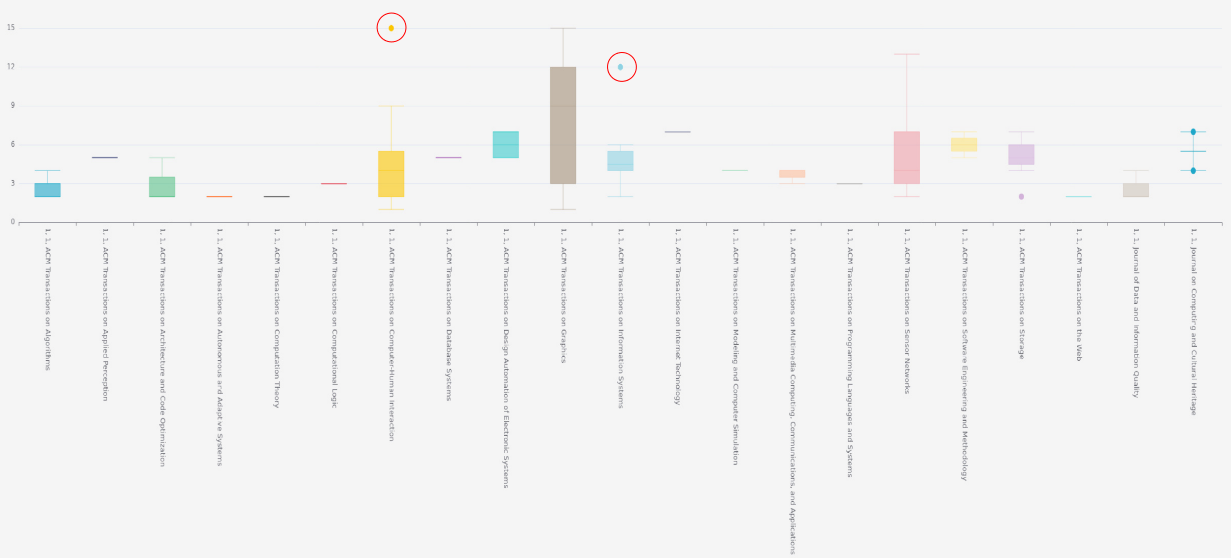
\includegraphics[width=16cm]{images/data_integration/editors/editors_coauthor_analysis.png}
%     \caption{Outlier analysis of the use of coauthors}
%     \label{fig:editors_integration_coauthor_analysis}
% \end{figure}
% Interesting to see is that for two journals outliers are identified (visible 
% with a red circle). 

% ==============================================================================
\section{Validation}
% \outline{
% \begin{itemize}
%     \item Werkt je methode
%     \item Aan het eind van ieder hoofdstuk of een eigen hoofdstuk
% \end{itemize}
% }
We can clearly see skewness in the number of unique coauthors between 
inside and outside the journal for a few editors; the notable observations were 
not exceptional at further analysis.
However, if we compare these observations with other editors in the population,
they do stand out.

Possible explanations are:
\begin{description}
    \item[No strange behaviour] There is no strange behaviour within the group 
        of editors.
    \item[Limited dataset] We only use data of 2020 for a few journals of ACM. 
        This set may be too limited and does not represent all editors. Outliers
        in the analysed dataset may be outliers within ACM, but not considering
        a larger population.
    \item[Wrong analysis] If authors publishes multiple times and they are 
        obliged to add the editor as coauthor, this will reflected in the 
        analysis.
\end{description}

% ==============================================================================
\chapter{Case study 3: Authors}
\label{chp:case3}
% ==============================================================================
In this chapter we dive into the authors. More specific; we look at the timeline
properties of a publication.

\section{Motivation}
The motivation to investigate this group from a timeline-perspective, is that
fraud had been detected using these properties. Also other research working with
timelines are successful~\cite{SNCMBL2021}. Scanff et al. investigated the 
relationship between the publication-lag and prolific authors, which may be a 
member of the editorial board. This study makes clear that dates about the
publication process are interesting features.  

We will proceed with an interesting case involving the timeline properties.
% ------------------------------------------------------------------------------
\subsection{Interesting case: Author reviews his own work}
\label{interesting_case:author_reviews_own_work}
An author that reviews his own work is off course a major attack on the
integrity of the publication process. It should never be the case that an author
becomes in a position where he can review his own work. Unfortunately, we know
of such case involving Hyung-in
Moon\footnote{\url{https://retractionwatch.com/category/by-author/hyung-in-moon/}}. 

In Figure~\ref{fig:air} we present an instance model of this situation. We have 
a person (pers1) who have multiple roles in relation to one publication (p2).

\begin{figure}[H]
\centering
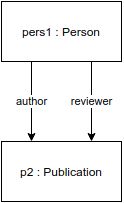
\includegraphics[width=3cm]{images/author_is_reviewer.drawio.png}
\caption{Instance model where author is also the reviewer}
\label{fig:air}
\end{figure}
% ------------------------------------------------------------------------------
From a set theory perspective we can describe this situation as: 
$\{h \in \Humans \mid \authors(p, h) \land \reviews(p, h)\}$.

In theory this situation can easily be detected. However, besides 
availability of the necessary data, the person executing such attack, will 
most likely not give his own name as reviewer at the moment of submitting his 
paper (it is 
normal to identify possible reviewers at submission~\cite{C2013}). The main
question here 
is, how are we able to identify the author and reviewer as the same person.

We approach this situation from a timeline perspective, which is how Moon is 
detected. A paper goes through certain stages until it is published. In
Figure~\ref{fig:timeline} we draw a timeline with the milestones of the
publication process. \textit{Submitted} is when the paper is received by the
venue. \textit{Revised} is the moment a paper is submitted again after review
with changes; the asterisks implies that this can occur multiple times, or none
at all if the paper is accepted at first submission. \textit{Accepted} defines
the state when the paper is ready for publishing. \textit{Published} is the last
step and is the date the paper is published.

Most publishers also work with an \textit{Available Online} date. Once accepted,
a paper can be placed on the website of the publisher before the journal has
been published.
% ------------------------------------------------------------------------------

\begin{figure}[H]
\centering
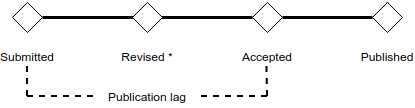
\includegraphics[width=9cm]{images/timeline.drawio.png}
\caption{Milestones in timeline publication model with publication lag}
\label{fig:timeline}
\end{figure}

The publication-lag is defined as the time between submission and acceptance.
This measure can be used as comparison with other authors en within 
the same venue. A low publication-lag compared with 'normal' can be used to 
identify interesting cases like an abnormal short time of review. E.g. Moon was
detected because the time his work was submitted and approved by the
reviewer (which was Moon himself) was remarkable short.
% ------------------------------------------------------------------------------
\paragraph{Beneign alternatives}
The possibility exists that a paper is that good, no revision is needed and the 
review did not take that much time. This also results in a low publication-lag.
% ------------------------------------------------------------------------------

\section{Data acquisition}
In this section we describe how we acquire the data necessary for this case
study.
% ------------------------------------------------------------------------------
\subsection{publication lag}
% ------------------------------------------------------------------------------
The publication date is an attribute well presented in public datasets. This 
date is derivated from the publication of the venue. 
To get the dates needed to calculate the publication-lag (submitted and
accepted), we need other sources. ACM and Elsevier show the dates on their
website (as example for ACM, see Figure~\ref{fig:acm_dates}). However, these
properties are not available for all publications.

\begin{figure}[H]
\centering
\includegraphics[width=5cm]{ACM_Digital_Threats_Research_and_Practice.png}
\caption{Publication history of an article in ACM (\url{https://dl.acm.org/doi/10.1145/3442445})}
\label{fig:acm_dates}
\end{figure}

As we already used ACM in the previous case study; in this case study we
use Elsevier. Besides we already used ACM, we have proved to be able to extract
the dates from the Elsevier website in the research proposal.

When Elsevier presents an article on their website, a JSON 
document with details about the article is available in the HTML document. Among
other details, this JSON contains a date section, see 
Listing~\ref{lst:ElsevierJsonDates}.

\begin{lstlisting}[caption={Dates in the JSON document},label={lst:ElsevierJsonDates}]
"dates": {
    "Available online": "25 January 2021",
    "Received": "16 July 2020",
    "Revised": [
        "14 December 2020"
    ],
    "Accepted": "4 January 2021",
    "Publication date": "25 January 2021"
}
\end{lstlisting}


% dit is nog can proposal... moet anders
By using web scraping and HTML interpretation we extracted the JSON documents 
with metadata of articles across 36 journals from Elsevier (Elsevier runs 2751 
journals). This resulted in a total of 35136 documents.

% We were able to calculate 
% the average publication lag per journal and filter on the articles for which the 
% publication lag was significant lower. A quick look at the editorial board of 
% that specific issue showed that one of the authors was indeed part of the 
% editorial board. Based on this small experiment, we conclude that it is 
% possible to get the publication lag for most articles of Elsevier journals.





% \begin{itemize}
%     \item Not all publishers expose the dates these stages are achieved. 
%     \item Fortunately some do. For example ACM (\ref{fig:acm_dates}) and Springer. However, this is not for all publications available. So there are some missing data points.
%     \item Fraud cases where this information can be helpful:
%     \begin{itemize}
%         \item Moon was detected because the time that his work was submitted and was approved by the reviewer (which was Moon himself) was remarkable short.
%         \item ~\cite{SNCMBL2021}
%     \end{itemize}
% \end{itemize}

From the 35136 we were unable to calculate the publication-lag for 12290
(approximately 35\%) because the date properties needed are missing.

% \section{Data integration}



% ==============================================================================
\section{Analysis}
% \outline{
% \begin{itemize}
%     \item Wat betekent de data?
% \end{itemize}
% }
In this section we present a possible method to analyse this data. We focus in
our analysis on the ACM journal Information and Software Technology
(\url{https://dl.acm.org/journal/inst}).

In Figure~\ref{fig:publication_lag_dist} we show the distribution of the
publication lag. The average is shown with a vertical red line, the median with
a black line. Every dot represents a publication.

\begin{figure}[H]
    \centering
    \includegraphics[width=\textwidth]{images/case_study_3/dist.png}
    \caption{Distribution of the publication lag.}
    \label{fig:publication_lag_dist}
\end{figure}

Because of the right skewness in this dataset, we transpose it with log10 to
create a set that is more normally distributed. 

In the publications we scraped from Elsevier, we noticed 190 observations with a
publication-lag of 0 (zero). Possible explanations are:
\begin{description}
    \item[Data quality] It can be that this is an error on the side of Elsevier.
    \item[Actually 0 publication-lag] Another explanation is that the
    publication lag is actually 0. This means the article is submitted and
    accepted on the same date. 
\end{description}
We need to make a choice what to do with these observations because we can not
calculate the log value of a 0 publication lag. Considering the domain we work
in it is
save to identify 0-values as outliers, because it represents an very fast
process from submission to acceptance, at least within one day.
To make sure these values are indicated as outliers, we replace $\log_{10} (0)$
with 0.

The result of this transformation is shown in
Figure~\ref{fig:publication_lag_dist_log}. We notice that the
average line and median are much closer.

\begin{figure}
    \centering
    \includegraphics[width=\textwidth]{images/case_study_3/dist_log.png}
    \caption{Distribution of the log of the publication lag.}
    \label{fig:publication_lag_dist_log}
\end{figure}

In Figure~\ref{fig:cs3_publag_iast} we plotted the log-values of every
publication-lag, ordered by author. Every dot represents a publication. The log
of the publication-lag on the y-axis. The x-axis is an order by name of the
author (for explanation see Section~\ref{sec:cs1_analysis}).

The red dots are identified as outliers (z-score > 3). 

\begin{figure}[H]
    \centering
    \includegraphics[width=\textwidth]{images/case_study_3/publication_lag_iast.png}
    \caption{Publication lag of authors of Information and Software Technology.}
    \label{fig:cs3_publag_iast}
\end{figure}

The red circle in the left lower corner, we identified a 'cluster'; one author
of which the publication-lag was two times very low; 8 and 11 days (average
270, standard deviation 115). 

In Figure~\ref{fig:cs3_pop_vs_poi} we compared the author of this cluster with
the population and an authors with more `normal' publication-lag duration. 
The publication-lags of the person-of-interest is outlined with a red dotted box
(the red striped around the two observations are the same as in
Figure~\ref{fig:cs3_publag_iast}).
In the green dotted-box we plotted the publication-lag times of an author which
behaves `more' normal.

\begin{figure}[H]
    \centering
    \includegraphics[width=11.5cm]{images/case_study_3/poi_vs_rest_vs_normal_crop.png}
    \caption{Log of the publication lag of population compared with person of interest and more `normal' author.}
    \label{fig:cs3_pop_vs_poi}
\end{figure}

An investigation of a possible relation between the person-of-interest and any
member of the editorial board did not return notable results. The authors of
these papers were not part of the editorial board, nor did we notice an editors
of the same affiliation of one of the authors.


% ==============================================================================
\section{Validation}
% \outline{
% \begin{itemize}
%     \item Werkt je methode
%     \item Aan het eind van ieder hoofdstuk of een eigen hoofdstuk
% \end{itemize}
% }
At this chapter we took data of Elsevier for a a subset of journals in the
domain of Computer-Science. Almost 34\% of the data we acquired from Elsevier 
was not usable for analysis. 

We investigated one journal and were able to identify a 
person-of-interest with two publications of which the publication-lag deviates
from other publications in the journal.

At this point we can conclude that we notice some very low, even zero, days 
between submission and acceptance of a publication. We are not able to say 
anything about the outliers. Further 
investigation can combine these properties of publication with data of editors (e.g.
is the author an editor, is the editor a colleague of the author). Another
direction to investigate can be a possible pattern in reviewers and publication-lag.
We did not found a source to get data of reviewers for a certain publication, 
but most of the times the reviewers are available at venue level (e.g. in the masthead).

% A limited mannual explorative analysis during the research preparation seem to 
% lay a connection between the editorial board and the publication-lag. We are
% unable to verify this on a larger scalen, because the data of the editorial
% board of Elsevier is not at our disposal.







% \begin{itemize}
%     \item Onbekend of deze methode werkt
%     \item Mogelijk te weinig data
%     \item Exploratieve analyse leken wel een verband aan te tonen tussen de
%     publication lag en de editorial board. With this case study it is not 
%     possible to verify this statement. The editorial board data for the analysed
%     journals are not acquired. 
%     \item For possible futher study; this may be a good statement to 
%     investigate.
%     \item Unable to say something about the found oberservations; we do not know
%     who is the reviewer. This data set is unavailable.
%     \item Initiative: Open Peer Review (\url{https://www.fosteropenscience.eu/})
% \end{itemize}

% ==============================================================================



% ==============================================================================
% \subsection{Roles in the editorial process}
% In the editorial process multiple roles are involved. These roles are executed
% by persons. We define all persons involved somehow in the editorial process by 
% \textit{H}. Publications are defined by the letter \textit{P}.
% % ------------------------------------------------------------------------------
% \paragraph{Author}
% \begin{itemize}
%     \item How evident, this role writes the text to be published.
%     The main question is, how is someone with this role able to influence the process in his favor.
%     One way is to suggest a reviewer and indicate non-preferred reviewers \cite{C2013}. This relates to the case of Moon.
%     \item Suggest Associate Editor
% \end{itemize}
% We define the collection authors of a paper $A(p) = \{h \in H \mid \authors(p, h)\}$

% % ------------------------------------------------------------------------------
% \paragraph{Editor-in-chief}
% Wie bepaalt wie de editor-in-chief is? -> macht
% \begin{itemize}
%     \item receives the manuscript $\receives(p, h)$
%     \item Performs initial check (relevance, suitability to undergo peer review)
%     \item Assigns Associate Editor based on Area of expertise and avoiding potential conflicts of interest between author and AE
%     \item end decision if paper is being published: Stel h = Editor in chief en p = publication dan: $\accepts(p, h)$ of $\rejects(p, h)$
%     \item An editor-in-chief has this role for a certain period (span multiple issues).
% \end{itemize}


% % ------------------------------------------------------------------------------
% \paragraph{Editorial assistance}
% \begin{itemize}
%     \item Checks similarity to other publication (iThenticate)
%     \item Verder geen invloed op process
% \end{itemize}

% % ------------------------------------------------------------------------------
% \paragraph{Reviewer}
% \begin{itemize}
%     \item Reviews a paper
% \end{itemize}
% We define the collection reviewers of a paper $R(p) = \{h \in H | reviews(p, h)\}$
% % ------------------------------------------------------------------------------
% \paragraph{Subeditor}
% \begin{itemize}
%     \item Niet echt relevant
%     \item Om tekst leesbaarder te maken
% \end{itemize}
% % ------------------------------------------------------------------------------
% \paragraph{Associate editor}
% \begin{itemize}
%     \item Identify and Assigns reviewers
%     \item administrative reject (desk reject): vaak al in eerder stadum eruit 
%         gehaald door Editor-in-Chief of Editorial assistance
%     \item recommendation to editor in chief
%     \item Following roles sometimes combined into the Associate Editor:
%     \item Managing editor
%     \begin{itemize}
%         \item Checks journal standards, word length, use of internal reporting 
%             standard
%         \item assigns editor
%         \item assigns reviewers
%     \end{itemize}
%     \item Editor
%     \begin{itemize}
%         \item Initial check
%     \end{itemize}
%     \item This role is also for a period of time
% \end{itemize}
% ------------------------------------------------------------------------------


% ==============================================================================
\chapter{Conclusions}
\label{chp:conclusions}
% ==============================================================================

In this research we set out to direct manual investigation to notable cases.
We conclude this research with the following key findings:

% ==============================================================================
\paragraph{It is not feasible to create an integrated dataset out of multiple
publicly available datasets}
Source depended keys (e.g. for identifying authors) are only applicable within 
that single dataset. Therefore integrating datasets should use 
source-independent key attributes (\doi{} and \orcid{}). Ideally datasets 
containing data of the publication process should include these attributes. In 
practice the quality and availability of these source independent keys is not 
sufficient for identifying objects (see Section~\ref{sec:data_integrability}). 
This impacts the quality of the resulting integrated dataset.

Alternative approach to use names instead of \orcid{} for identifying objects are 
not sufficient. However, it is possible to use alternative approaches 
(see Aminer~\cite{Tang:08KDD}); achieving a high enough level of quality 
requires a lot of effort. For the purpose of our research, we therefore conclude 
that creating an integrated dataset for analysis purposes is too cumbersome.
% ==============================================================================
\paragraph{Enriching standard datasets is made more difficult because of the 
lack of structured data}
Standard available datasets are based around the author, paper, venue and 
sometimes the citation. These datasets are insufficient for generic outlier 
detection~\cite{TEJ2017}. Therefore, this research aim to use a group based 
approach.

Standard datasets miss data to apply group based approach (e.g. data of PC 
members, publication-lag). In theory this data is publicly available, mostly on 
the website of publishers. In practice, this data is in an unstructured form.
Due this unstructured form, acquisition of this data and integration with
existing datasets is challenging. For example, our proof-of-concept PDF data
extractor, specifically tailored to its source material, still only achieved
a success rate of $\sim$47\% for extracting data.


% ==============================================================================
\paragraph{Applying group based approach on enriched data yields useable results}
We executed three case studies to investigate if applying a group based approach 
can indicate notable cases for manual investigation.

In the first case study we gathered the PC members from \lncs{} front matter 
documents and combined this data with \dblp{}, OpenCitations and scraped data 
from Springer Website. As an example analyses we looked at how often these 
members where cited in their own journal. For one proceeding we plotted the 
results in Figure~\ref{fig:analysis_members}. We can clearly identify an 
outlier.

% ==============================================================================
In the second case study we acquired the Editorial board of ACM journals. This 
data is combined with \dblp{} to get the co-authors. As a possible analysis 
method, we looked at the number of unique co-authors these editors worked with 
inside versus outside the journal. In Figure~\ref{fig:editors_in_out_journal} 
the results of one journal are shown. Although not as clear as case study 1, we 
are able to direct manual investigation to notable cases (especially point 3).

% ==============================================================================
As third case study, we focused on the time aspect of the publication process by 
looking at the publication-lag. In this case we did not integrate additional 
data. Instead of indicating the value of additional objects, we show the value 
of additional attributes for already available objects in standard datasets. We 
used data of some journals we scraped from Elsevier. In 
Figure~\ref{fig:publication_lag_dist_log} we see the deviation of the 
publication lag. On the left side we notice very low publication-lags. We 
consider this valuable information for a publisher to investigate some 
publications.

\ \\
In all these cases we were able to show that adding public data to standard 
datasets results in notable cases, which can (and probably should) be 
investigated. Therefore we conclude that applying a group based approach on 
enriched datasets works.


% \section{OLD}



% The main question of our research was: 
% \textbf{How can integration of public available data sources improve the
% detection of scientific fraud?}

% Our assumption based on previous work was that by extending public available
% datasets with additional data we should be able to identify interesting people
% involved in the publication process.

% We investigated how we could formalise an integrated datamodel and load this
% with additional data. In Chapter~\ref{chp:data} we formalised a logical entity
% model of the publication process.
% We were unable to create a physical integrated dataset because data quality is 
% an issue. 

% Publicly available datasets and additional data do not (or partially) contain 
% necessary attributes to integrate multiple datasets. The most important 
% attributes in this case are the \doi{} and the ORCID.

% Too be able to still prove if our assumption is correct, we continued by taking
% a more pragmatic approach with the case studies.

% \paragraph{Case study 1}
% During the first case study we acquired PC member data from LNCS
% (Chapter~\ref{chp:case1}). To get this
% data we built software to process and interpret the front matter
% documents of the proceedings (Chapter~\ref{chp:front_matter_parsing}). We 
% formalised a dataset to gain statistics about articles published in
% the proceeding that cites work from PC Members, too see if we can 
% identify forced citation. We also demonstrated how to compose a dataset with the number of publications the PC members publish in their own proceedings.

% In the analysis phase our scope was one journal. Analysis resulted in the
% identification of an outlier in the citation dataset. Although we
% are unable to conclude this is a form of forced citation, we were able to
% identify the PC member which metrics differ significantly compared to his
% peers.

% Possible directions for further research are:
% \begin{itemize}
%     \item Identify how work is cited. Does it occur in a list, or is it a 
%     key-publication the work is based upon?
%     \item What are the publication dates of the work that is being cited? If
%     work that is being cited is not published yet, this may increase the 
%     possibility of fraud.
% \end{itemize}

% \paragraph{LNCS PC Members scraper}
% During case study 1 we built a proof of concept of software that parses
% \lncs{} front matter documents. Although not perfect, with only the limited amount of validated
% data we acquired this way, we already be able to address interesting members.

% \paragraph{Case study 2}
% We continued with journal editors from ACM. As an example of integration and
% group based analysis we looked at the difference between the number of unique 
% coauthors these editors worked with inside and outside the journal.

% Although we were not able to identify very strange behaviour, we do demonstrate
% a possible analysis strategy.

% Further research in this direction should be based on a larger dataset and may
% include data of groups of authors. Aminer uses this data to identify an author
% as being unique, so this data can may be acquired form Aminer (Academic Social
% Network).

% \paragraph{Case study 3}
% In case study 3 we looked at the publication-lag acquired from 36 journals
% of Elsevier. We are able to identify outliers in this set. However, we can not
% exmplain why these observations are outliers.

% Further research can look at other publishers, like ACM, or include data from
% open review collaboration sites.

% \paragraph{}
% The limitations of the results of the above described cases are that these can never
% classify an author as an fraud; this should always be a human judgement.

% \subsection*{Key findings}
% Based on the previous points we formulate our key findings as:
% \paragraph{$\blacksquare$ Creating an integrated dataset is not possible due lack of data availability and data quality}
% The main entities involved in the publication process are widely available (author, paper, venue).
% However, other roles, with a lot of influence in the process, are not available (see Section~\ref{subsec:ConclusionsDataAvailablity}, \nameref{subsec:ConclusionsDataAvailablity}). 

% Creating one integrated comprehensive dataset is not possible because the lack of quality of source independent properties; the \doi{} and ORCID.
% \paragraph{$\blacksquare$ Adding data and applying a group based approach improves detection of outliers}
% By acquiring PC memberships, editors and publication dates, we were able to indicate interesting cases during a limited analysis that could be further investigated. 

% In Figure~\ref{fig:analysis_members} we show the results of an analysis based on PC memberships; one author clearly stands out of his peers. In Figure~\ref{fig:editors_in_out_journal} we show the ratio of unique authors editor work with. Although no case really stands out, no. 3 is a bit curious.

% We indicate that the publication-lag is a very interesting property. Although we did not combine this with additional data, only having this property already results in outliers as shown in Figure~\ref{fig:cs3_publag_iast}.

% % \end{itemize}
% ==============================================================================
\paragraph{Impact of this research}
The conclusions and part of the approach of this study can result in a detection
framework that directs investigation of fraud to the most striking cases. This
improves the detection of fraud cases which eventually results in a more fair
scientific publication environment.
% ==============================================================================

\section{Future work}
We present three directions for further research: Data acquisition, Data 
integration and an alternative data structure.

\subsection{Data acquisition}
This research shows the added value of additional acquired data; PC members from 
Springer LNCS, Editors of ACM and publication-lag of Elsevier. However, these 
datasets has their weak spots which could be improved. 

In this section we propose some improvements in data and process.

\paragraph{PC Members}
In this study we built a proof-of-concept to parse the front matter of Springer 
LNCS. Improving (or rebuilding) this tool to create a more sustainable solution, 
would improve the dataset and eventually lead to more data with a higher quality. 

Research could be conducted if the same approach and software can be applied to
load documents from other publishers (e.g. IEEE).

\paragraph{Editorial board}
The added value of having data about the Editorial board has been mentioned 
multiple times by other researchers. In our research we used webscraping to get
the editorial board of a limited number of journals from ACM. Our approach has a 
few weak spots:
\begin{itemize}
    \item The data is limited to journals of ACM;
    \item Only the active board is acquired.
\end{itemize}
A solution that would acquire editorial board documents (comparable with the 
LNCS front matter documents) and parses these documents, would deliver high 
added value to the research in scientific fraud.

\paragraph{Review data}
Data about the review process is not publicly available. However, if we look at
the publication process, this review part has a high impact on the scientific 
performance of authors. Therefore, data about this process is valuable.
Open initiatives to review papers do exist. One of them is
Pubpeer\footnote{\url{https://pubpeer.com/}}, 
where researchers can comment on papers.
Mining this data adds value about the quality of publication process of 
venues.

\paragraph{Industrialise data acquisition}
In this research we acquired the data as a one-time effort.
This results in pieces of a data pipeline.
When directing for a general safety net, a more structured approach should be 
set up. We propose two directions necessary for this safety net:
\begin{enumerate}
    \item The pieces of the pipeline should be chained together to form a
        a more streamlined process;
    \item Loading complete datasets every time is cumbersome. Therefore acquiring 
    delta’s could improve performance of the detection process.
\end{enumerate}

\paragraph{Front matter parsing}
From the validation of the front matter parsing proof-of-concept
(Chapter~\ref{chp:front_matter_parsing}) it is clear that improvements are 
possible. This will result in a better parsing and therefore in more and better 
data.

However, this is still a quick win: only name and affiliation are available in 
these documents and formats can and will change. Our assumption is that 
continuing this approach, the amount of acquired data will not exceed the 80\% 
of available data in the front matter documents.

Therefore, the need for a machine readable standard (see recommendations) stays, 
but this direction does improve the analysis on short-term; resulting data will 
certainly be better than what is available right now.

\subsection{Dataset integration}
In this research integrating multiple datasources to create one dataset was not
feasible. One reason is that people involved in the publication process were not
uniquely identifiable.
Possible directions to improve the integration of people are:

\paragraph{ORCID as source}
In this research we approached integration directed from the datasources, which
may contain an \orcid{} for the author. In Figure~\ref{fig:fw_orcid_1} this is 
drawn on the left side. Another approach may be to see the \orcid{}
as source, and match people based on their publication (in \orcid{} people can 
add their publications) \textit{or} \orcid{}, shown on the right. In this new
situation, \orcid{} becomes a bridge between the sources.

\begin{figure}[H]
    \centering
    \includegraphics[width=14cm]{images/conclusions/fw_orcid_1.png}
    \caption{Left: our approach, right: proposed improvement}
    \label{fig:fw_orcid_1}
\end{figure}

\subsection{Alternative detection method}
The focus of this research is on the added value of integrating additional data 
sources. The case studies to prove this value were all executed with attacks in 
mind. Therefore, the datasets created for this analysis were focused on certain 
metrics to indicate these attacks. 

The weakness is that this approach is
still specific to each attack: for every new type of attack discovered, a new
analysis or detection method has to be implemented. 
To discover these new attacks, the community ends up relying on whistleblowers, 
which essentially brings us back to square one; no generic approach.

Our proposal is to look at the structure of the data from a graph 
representation. In Chapter~\ref{chp:graph_based_approach} we will perform an
initial exploration on this approach.

% \section{CONTINUE HEERRRREEEEE!}
% \todo{heelveel}
% voorzet, misschien generieke methode mogelijk

% generiek werkt niet op data zelf
% mss wel op graaf representatie, in volgende hfst

% nu nog steeds kijken welke outliers we geintreseerd zijn
% tielenburg? misschien outcount niet goed genoeg

% voorstel kijken naar cycle


% ==============================================================================
\section{Recommendations}
\label{sec:recommendations}


The most recommendations we present are for the publisher.

\paragraph{Machine readable standard}
As we shown in this research, currently valuable data is available, but:
\begin{itemize}
    \item In an unstructured manner (some in PDF documents, e.g. editors, some 
        data on website e.g. dates);
    \item Every publisher provides this data differently.
\end{itemize}
This results in problems acquiring this data:
\begin{itemize}
    \item Lots of publisher-fitted procedures should be implemented;
    \item It is not possible to separate between data not known, or data not 
    presented.
\end{itemize}
% ==============================================================================
This last point is important. Consider the following two structures to represent 
a person. In Listing~\ref{lst:rec_ex_not_known} the ORCID element is 
provided, but it is not known. The receiver (client requesting this data) knows 
that the ORCID is not known by the sender (which is eventually also information 
about data-completeness). In 
Listing~\ref{lst:rec_ex_not_present}, it is unknown if the sender knowns the 
ORCID, but is not presenting it, or if the sender don't know the ORCID, and 
therefore not sending this value.

\begin{lstlisting}[
    caption={Example of not known data},
    captionpos=b,
    label={lst:rec_ex_not_known}
    ]
    "Person": {
        "FirstName": "Jodocus",
        "LastName": "Kwak",
        "ORCID": null
    }
\end{lstlisting}

\begin{lstlisting}[
    caption={Example of not presented data},
    captionpos=b,
    label={lst:rec_ex_not_present}
    ]
    "Person": {
        "FirstName": "Jodocus",
        "LastName": "Kwak"
    }
\end{lstlisting}

Therefore, our recommendation is to define a machine-readable standard for data 
exchange with no optional fields (values can be null).

With a standard in place, more research based on improved data can be conducted, 
which eventually leads to more fraud detected.

% ==============================================================================
\paragraph{Apply fraud detection on the process}
Currently automatic fraud detection procedures are in place for publication 
content, e.g. plagiarism. On the publication process side, most publishers have 
a code of conduct. However, we are unaware if automatic detection of fraudulent 
behavior is in place.
% ==============================================================================
Therefore, our recommendation is to:
\begin{itemize}
    \item Make detection of fraudulent behavior an integral part of the 
        publication process;
    \item If procedures are in place, provide information to the public that the 
        publication process is being monitored for fraudulent behavior.
\end{itemize}

The result is that people with malicious intent are become restrained in 
attacking the publication process.

% ==============================================================================
\paragraph{Make more data about the review process public}
Data about the review process is not publicly available. However, this review 
process is essential for the scientific community; this is the 
`self-controlling’ element which leads to a certain research quality.

This is also a weak spot; the result of the review entirely depends on the 
reviewer, which may, or may not, be personally involved.

Therefore our recommendation is to provide metadata about the review process, 
e.g:
\begin{itemize}
    \item Who reviewed which paper;
    \item When was the paper presented to the reviewer;
    \item When was the result of the review returned;
    \item What was the result.
\end{itemize}

Providing this data to the community will result in monitoring the review 
process on personal involvement and therefore forces the review to become 
more about the research instead of the researcher.

% ==============================================================================
\paragraph{ORCID}
During analysis of the scraped data from Springer, we ran into cases where an 
author has multiple ORCID's. Checking these ORCID's at \url{https://orcid.org/} 
made clear that these are indeed the same person, but working at different 
universities.
Our recommendation for researchers therefore is to use one ORCID consistently.

% \paragraph{Make more data available}
% For publishers it is little effort to make more data available. As example, the
% dates of the publication process to get the publication-lag is available for
% publishers and is a major enrichment of existing datasets.

% \paragraph{Make data machine-readable}
% It would be a major improvement if publishers make data of editors and PC
% members machine readable available. As of now, the documents (front matter,
% editorial notes) containing these people do not include the ORCID. This makes,
% sense, the document is meant for humans, but for data integration and analysis
% purposes, this would be a big improvement.

% \paragraph{Improve (and measure) data quality}
% One conclusion is that due to lack of data, we were unable to create an
% integrated dataset. The two attributes to start with should be the ORCID and
% DOI. Detection should be in place to detect if a person has multiple ORCID's,
% or none. A sanity check can be put in place if the ORCID delivered by the author
% is correct by cross-referencing \url{https://orcid.org/}.

% \paragraph{Stick to one ORCID}
% During analysis of the scraped data from Springer, we ran into cases where
% an author has multiple ORCID's. Checking these ORCID's at
% \url{https://orcid.org/} made clear that these are indeed the same person, but
% working at different universities. Therefore, for authors; please stick to one ORCID.

% \paragraph{Apply more fraud detection by publishers}
% \label{p:recom:fraud_detection_publishers}
% Due incorporate quality assurance in the publication process and propagate this
% to the community, the value of publishing at a venue of this publisher may
% increase, which is beneficial for all venues of the publisher.
% If the value increases, other publishers will be forced to also take action
% which results in less fraud altogether.

% ==============================================================================
\section{Discussion}
\label{sec:discussion}

% \paragraph{Automatic detection of fraud in the publication process}
% Because the publication process always involves human interaction, we should 
% always ask for explanation when curious behaviour is detected.


In this research we found that enriching datasets with publicly available data 
increases the detection of outliers in the publication process. This means that 
valuable data is `hidden’ in PDF documents and shown on websites. 

That we can detect outliers does not mean that we can detect fraud, we can only address outliers. As 
stated in the introduction, the underlaying assumption of this research is that 
fraudulent behavior will be reflected as outliers, but not all outliers are 
fraud. This raises the question raises if we ever be able to set up a system 
that detects fraud in the scientific publication process. In our opinion, we 
should always apply for fair hearing.


Our main goal was to propose an approach to direct manual investigation to 
notable cases. Theoretically, this approach can be applied for that goal. 
However, we are unable to determine if this actually results in finding frauds. 
A more comprehensive study with current ‘catches’ compared with investigation of 
outliers found by our proposed approach should provide the conclusion if this 
approach pays off.

We can not state that we find an enormous number of interesting cases; this 
depends on the threshold that defines the outlier. However, the threshold we 
put in place during the case studies were high. Investigating the list of 
outliers from most to least, will eventually reach a point that investigating 
does not pay off anymore. The border before that moment can be set as a 
threshold. Only then we know how successful our approach is in actually 
finding frauds.




% ==============================================================================

\paragraph{Addressing cross-publisher fraud}
% ------------------
Current fraud detection mechanisms typically focus on the content of the 
publication. However, as argued in this thesis, data on the publication process 
may be leveraged to uncover forms of fraud that have escaped notice so far. One 
example of such a fraud is `lightweight' fraud that is repeated across many 
publishers. This fraud becomes impactful due to the quantity of affected works, 
not the impact of a single fraudulently published work.
Addressing such fraud requires at the very least integration of data from 
different publishers.

% As stated in the recommendations; unprecedented behaviour should be detected by publishers. However, some forms of
% fraud are across multiple publishers. As for now, some enthusiastic researchers and sites (e.g. Retraction Watch\footnote{\url{https://retractionwatch.com/}}) dive into these topics, but maybe we (you),
% as in the research community, should address an institute that is responsible for cross-publisher detection of fraud.

% ==============================================================================
A solution could be an independent institute which receives the necessary data 
to do cross-publisher analysis. This institute could serve as a provider for
analytical services for publishers unable to set up this necessity themselves.

The responsibility of this institute is to address and investigate notable 
cases.



% A possible setting is that the publishers delivers data to this institute, this institute analyse the data and returns their findings. If this institute give out some kind of statement to the publisher, it may becomes a quality status for all publishers.
% The more publishers make use of this organization, the more data is available and fraud will be detected.

% Eventually, this leads to damage of the image of publishers if they do not cooperate. Is that an acceptable situation?

% ==============================================================================

%     \begin{itemize}
%         \item Op generieke manier wetenschappelijk fraude detecteren, kan dit automatisch?
%         \item Misschien meer data
%         \item Imago schade als publishers niet meewerken
%     \end{itemize}
% One way to decrease fraud in the publication process is to step away from the
% current way of judging a researcher. The University of Utrecht is moving to 
% another method to judge their researchers based on their effort to promote open
% research and their teamwork 
% \footnote{\url{https://www.nature.com/articles/d41586-021-01759-5}}. With this 
% movement the university is abandoning the indices based on publications and 
% citations.
% \begin{itemize}
%     \item Hoe kan men dan oordelen waar budget heen moet?
%     \item Hoe beoordeelt men de toegevoegde waarde van een onderzoeker 
%     objectief?
%     \item Wat is de impact hier van op de 'piramide'-structuur van 
%     universiteiten?
%     \item Hoe kunnen medewerkers bij de UU de overstap maken naar een 
%     universiteit die beoordelingen wel basseren op impact factor?
    
% \end{itemize}





% \outline {
% \paragraph{meer data openbaar maken}
% \begin{itemize}
%     \item bijvoorbeeld publicatielag
%     \item Niet spannend (weinig moeite voor publishers), wel grote verrijking
% \end{itemize}
% \paragraph{Meer fraud detectie inzetten door publishers}
% \begin{itemize}
%     \item Kwaliteit van dit stukje van het publicatieprocess borgen.
% \end{itemize}
% }



% \outline{
% \begin{itemize}
%     \item Samenvatten
%     \item Niet alleen samenvatting!
%     \item Wat is de impact op de wereld? Wereldvrede :)
%     \item Wat zouden we moeten doen en hoe kunnen hiervan profiteren?
%     \item Misschien combineren met Discussions?
%     \item Voorbeeld discussions
%     \begin{itemize}
%         \item Op generieke manier wetenschappelijk fraude detecteren, kan dit automatisch?
%         \item Misschien meer data
%         \item Imago schade als publishers niet meewerken
%     \end{itemize}
%     \item Misschien combineren met recommendations
%     \begin{itemize}
%         \item Informatie machine-readable aanleveren
%     \end{itemize}
%     scientific repeat.
% Conclusions repeat the key findings... *and* their impact. Typically, the impact is more important than the main findings. For example, "we found 37 sites out of 50 were vulnerable" is what you did. To that, you add what this means: how worrisome is this? what should be done now that we know this? How can we improve the world?
% \end{itemize}



% \section{Discussion}

% }



% % ==============================================================================
% \chapter{Recommendations}
% \label{chp:recommendations}
% % ==============================================================================
% \outline {
% \paragraph{meer data openbaar maken}
% \begin{itemize}
%     \item bijvoorbeeld publicatielag
%     \item Niet spannend (weinig moeite voor publishers), wel grote verrijking
% \end{itemize}
% \paragraph{Meer fraud detectie inzetten door publishers}
% \begin{itemize}
%     \item Kwaliteit van dit stukje van het publicatieprocess borgen.
% \end{itemize}
% }


\chapter{Exploration of abstract graph-based approach to outlier identification}
\label{chp:graph_based_approach}
% ==============================================================================

This proposal is to find a common denominator across attacks by approaching the 
publication process domain from a graph perspective.

Figure~\ref{fig:graph_1} shows a graph representation of self-citation.
Note that this is a 3-cycle directed graph: a person (node) authors (edge) a 
paper (node) which cites (edge) a paper (node) written by the same author (the 
first node).

\begin{figure}[H]
    \centering
    \includegraphics[width=8cm]{images/conclusions/future_work_graph/1.png}
    \caption{Graph representation of self-citation}
    \label{fig:graph_1}
\end{figure}

For readability we flatten this graph in Figure~\ref{fig:graph_2}. These are 
exactly the same situations. Person A on the left is the same as Person A on
the right (dotted line); in this chapter this notation is used to represent
the same node.

\begin{figure}[H]
    \centering
    \includegraphics[width=8cm]{images/conclusions/future_work_graph/2.png}
    \caption{Graph representation of self-citation, flatten}
    \label{fig:graph_2}
\end{figure}

If a person `attacks' the publication process by an exorbitant number of 
self-citations, this graph would extend as in Figure~\ref{fig:graph_3}.

\begin{figure}[H]
    \centering
    \includegraphics[width=8cm]{images/conclusions/future_work_graph/3.png}
    \caption{Graph representation of multiple self-citations.}
    \label{fig:graph_3}
\end{figure}

As such, the representation of a person that publishes in the venue he is 
editor of, is shown in Figure~\ref{fig:graph_4}.

\begin{figure}[H]
    \centering
    \includegraphics[width=8cm]{images/conclusions/future_work_graph/4.png}
    \caption{Graph representation of publishing in own journal.}
    \label{fig:graph_4}
\end{figure}

This situation can be extended as in we did in Figure~\ref{fig:graph_3}.


\newcommand{\ewcount}{\mi{count}}
\paragraph{}
In this research, an outlier is defined a an observation which matches or 
exceeds a thresholds; we define what is considered normal behaviour and 
indicate outliers. Now lets consider the following situation:
\[ \text{Let}\ A1=\text{self-citation attack (Figure~\ref{fig:graph_2})}. \] 
\[ \text{Let}\ A2=\text{self-publishing attack (Figure~\ref{fig:graph_3})}. \] 
\[ \text{Let}\ x=\text{outlier treshold set to 3}. \]
\[ \text{Let}\ \ewcount(A1)=2. \]
\[ \text{Let}\ \ewcount(A2)=2. \]

If we apply detection mechanisms as described in this research, both attacks 
are not considered an outlier (because $2 < 3$).
However, for the person applying these attacks, the total of `gains' he has
is 4 ($\ewcount(A1) + \ewcount(A2)$). Attackers who take these thresholds in 
account (and therefore stay under the radar), will not be detected. This 
situation is represented in Figure~\ref{fig:graph_5}.

\begin{figure}[H]
    \centering
    \includegraphics[width=11cm]{images/conclusions/future_work_graph/5.png}
    \caption{Two types of attacks.}
    \label{fig:graph_5}
\end{figure}

We see 4 paths, 2 for every attack; so considering the threshold $x$, this 
should be an outlier. 

A person will attack the publication process to improve its own metrics.
Therefore, the assumption that this future work proposal is based upon, is
that an attack can be considered a path from and to the 
same person. In 

An abstraction of this fraud detection approach is shown in 
Figure~\ref{fig:graph_7}; an attacker as Node A which performs $N$
attacks, visualized by the paths $1$ till $N$.

\begin{figure}[H]
    \centering
    \includegraphics[width=8cm]{images/conclusions/future_work_graph/7.png}
    \caption{Abstraction of paths.}
    \label{fig:graph_7}
\end{figure}

\newcommand{\incoming}{\mi{incoming}}
\newcommand{\outgoing}{\mi{outgoing}}
\newcommand{\isperson}{\mi{isperson}}
\newcommand{\isaffiliation}{\mi{isaffiliation}}
\newcommand{\isjournal}{\mi{isjournal}}

Considering this abstraction. We can set the following:
\[ \text{Let}\ n=\text{Node}. \] 
\[ \text{Let}\ p=\text{Path}. \]
\[ \text{Let}\ \isperson(n)=n\text{ is of type person.} \]
\[ \text{Let}\ \outgoing(n, p)=\text{path }p\text{ is outgoing of node }n\text{.} \]
\[ \text{Let}\ \incoming(n, p)=\text{path }p\text{ is incoming in to node }n\text{.} \]

The count of collection of paths of a person which eventually returns to 
the same person can than be expressed with Predicate~\ref{eqn:path_count}.
\begin{equation}
\label{eqn:path_count}
\forall n (\isperson(n) \implies \forall p(\outgoing(n, p) \land \incoming(n, p)))
%%\caption{Counting paths.}
\end{equation}


\paragraph{Benefits}
This approach has the following benefits:
\begin{itemize}
    \item At forehand specified derived metrics are not necessary (e.g. 
        \textit{count of citations} or \textit{count of publications}), the only 
        interesting metric becomes the \textit{count of paths}.
    \item \textit{How} the publication process is being played becomes less 
        relevant for detection. This approach indicates \textit{that} the 
        process is being played. Although this should not neglect the analysis
        of the attack to gain knowledge of attacks.
    \item Changing the \isperson() to \isjournal() or even \isaffiliation(),
        abstracts the type of the attacker. With this approach 
        attacks of journals to improve their Journal Impact Score or 
        affiliations that behaves like a high performing research facilities can
        be investigated.
\end{itemize}

\paragraph{Caveats}
This approach comes with some caveats:
That fact we reason about a directed graph is important. Also, the 
roles of the edges should not taken lightly. For example: If a person
\textit{authors} an article, the article is \textit{written by} that person. 
Theoretically, this
results in a cycle which will be counted in Predicate~\ref{eqn:path_count}.
  
\begin{figure}[H]
    \centering
    \includegraphics[width=5cm]{images/conclusions/future_work_graph/8.png}
    \caption{2-Path cycle to neglect.}
    \label{fig:graph_8}
\end{figure}

To prevent this, some measures should be taken. E.g.:
\begin{itemize}
    \item Set a minimum count of edges (neglect paths with less than 3 edges);
    \item Set a guard on the label of edges that inputs and outputs an attack.
\end{itemize}


% ==============================================================================
%\chapter{References}
% ==============================================================================


% ==============================================================================
% End of the line.... woohooo!
% ==============================================================================

\backmatter
\pagenumbering{roman}

\bibliographystyle{alpha}
\bibliography{report}


% % ==============================================================================
% \chapter{Appendices}
% % ==============================================================================
% \outline{
% Saaie dingen die er wel in moeten
% }

%% Use letters for the chapter numbers of the appendices.
%\appendix
\appendix
%  \input{Appendices/appendix-a}
%  \input{Appendices/appendix-b}
%  \input{Appendices/appendix-c}


% \chapter{VANAF HIER ONZIN}

% % ==============================================================================
% \section{General process}
% Bjorn and hedlund descirbed the publication process from a cost perspective 
% \cite{BH2004}. We can use this to visualize the publication process from a time 
% perspective. This view is input to determine if we are able to collect all 
% necessary metrics.



% % ==============================================================================
% \section{Flow proceedings and conferences}


% % ==============================================================================
% \subsection{Group identification}
% % ==============================================================================
% The first step in detecting outliers is to identify groups of people who are in 
% the same position. We identify the followig groups in his research because they
% may be interesting.

% \paragraph{Editors of proceedings}

% \paragraph{Authors submitting at the same conference}

% \paragraph{Author submitting at the same journal}

% \paragraph{Authors that publish with each other}

% \paragraph{H-Index}



% % ==============================================================================
% \chapter{Data integration}
% % ==============================================================================

% \section{References}



% \subsection{Hiding our identity}
% \vraag{waar moet dit}

% In this research we scrape a lot of data from websites.
% During our research preparation we got blocked by Science Direct 
% because we scraped the site with the same IP. To work around this problem of 
% being caught, two options exists.

% The first option is the use of a Virtual Private Network. Some free VPN 
% providers exists and scraping sites using a VPN hides the IP for the website; 
% the website only got the IP from the VPN server. The drawback is that the VPN
% provider may get blocked.

% The second option is using the TOR project as a proxy. TOR is a network of 
% servers that hides the identity from the requester. It also encrypts the 
% connection and is used during the Arab spring to reach social networks. This 
% TOR project is also known of the `Dark net' and certain illegal activities.

% For our purpose we choose to use the TOR network because we can programmaticaly
% change the route after a certain requests and free VPN servers are slow and 
% limited available.



% \section{Integration}
% People, articles and venues are retrieved
% from multiple source. To be able to work with these entities, we need to 
% integrate these sources in one model. To make this possible, we need to 
% unqiquely identify the entities.

% Again refering to Figure~\ref{fig:dataflow_jm2017}, we can consider this the 
% tilde sign.

% In the ideal situation al entities have an unique identifier which is 
% independent of the source. However, in practice it is a bit more complex than 
% that.



% \subsection{Articles}
% For all chapters from Springer LNCS we scraped the unique document identifier 
% (DOI). DOI should be unique of all documents.

% However, an analysis of the DBLP data set leaves us with a few DOI's which refer
% to mutliple articles. The number of articles this occurs, is very low.

% DBLP also has a lot of documents where the DOI is unknown; so data completeness 
% is an issue here. 

% For references we use opencitations. Because opencitations is DOI based, it is 
% very good integreerbaar with LNCS.

% % === oud, weg misschien
% % However, this document id is not filled in for all titles. For
% % the papers that do not have an doi, we can do the match on title. Unfortunately,
% % this also is not that straightforward. The title sometimes contains latex 
% % specific characters, or other weird characters.


% \subsection{Uniquify people}
% The author dataset contains all authors for every article. This means, if an 
% author wrote multiple articles, it is multiple times present in this set. For
% our use case, this is not sufficient; we need identify these people as the same 
% person, otherwise collecting metrics for a person is impossible.

% The set we achieved from LNCS conains name, orcid and email. An analysis of this
% set made clear that we got the same name with multiple orcid, or one orcid that 
% refers to more than one person. Concluding: a name does not make a person 
% unique.

% Luckely, DBLP acknowledges this problem. Although they do not yet have all 
% authors unique, they are working on this problem and provide a way to get the 
% unique persons already identified.

% DBLP has the relation between author and article, so to get the `correct' author
% of an article, we need to match the articles in DBLP with the chapters in LNCS.


% % \subsection{Article integration}
% % Not only do we need to match the articles of DBLP and Springer LNCS, we also 
% % need to incorporate Aminer. Aminer is an enrichment of DBLP in that it adds
% % citations. Although DBLP is working to incorporate citations in their dataset,
% % this is still work in progress and Aminer has already a lot of that data.

% % \begin{figure}[H]
% %     \centering
% %     \includegraphics[width=10cm]{images/linking_article_dblp_lncs_aminer.drawio.png}
% %     \caption{Matching Springer LNCS, DBLP and Aminer}
% %     \label{fig:linking_article_dblp_lncs_aminer}
% % \end{figure}



% \section{Nog onbenoemd}


% To get an integrated dataset across all sources some challenges need to be 
% addressed. Also, to be able to integrate the sources where we need to get the
% data from, we sometimes need to get data from another source.

% The main entities we need to integrate are person (authors, members of program
% committees etc.) and articles (chapters from lncs with papers from aminers).

% \section{Integration of persons}

% First challenge is to make the authors unique. This comes with the
% second challenge of data quality.

% For example, from springer we scrape get the chapters (inproceedings) and their 
% authors from their site. This authors sometimes comes with an orcid, which 
% should be unique. However, we found situations where an author gets an orcid of
% someone else. This is a data quality issue.

% Luckely, this does not occur much, and for the few it occurs we can easily 
% create a manual file to override this. Of course with caution; if two orcid 
% have the same name, we can not override this; some authors have the same name.
% On the other hand, if one orcid refers to a totally different name, we can.


% Seconds challenge is that a name does not make an author unique. The same name
% refers to other authors. Luckely, DBLP addresses this problem by suffixing the
% name with a four digit code~\footnote{\url{https://dblp.org/faq/1474704.html}}.
% DBLP is making progress here, but this is not entirely done yet. But even if
% they mention to unique identity authors, the match to authors in other 
% datasources (like Aminer and Springer) is not straightforward. In that case we 
% need to ignore the authors from these sources and make the match by going 
% through the paper (or chapter, as is it is called within LNCS Springer).

% Third challenge is the name. For most authors these sources do not contain an
% orcid or an email address, which means we need to match the authors on name.
% But, in some sources the names are fully written (with or without the 
% middlename), sometimes the middlename only has a initial while the firstname is 
% fully written, and sometimes we only get the initials and lastname.
% DBLP covers this by naming all aliases of a single person.

% Still we do have a problem, because inthe end we need to match these authors
% with members we get from the frontmatters of lncs. Within this frontmatters, 
% there is no orcid, email, or a four digit number to match to dblp records; these
% documents or not written with the intention to identify persons.

% \subsection{Approach}
% \begin{itemize}
%     \item Get DBLP data dump and create unique authors. DBLP also has their 
%         aliases and sometimes orcid.
%     \item Also use this dump to get the inproceedings, incollections and 
%         articles.
%     \item This dump can also be used to create the author relationship between 
%         articles and persons.
%     \item Integrate springer lncs chapters into the article entity.
%     \item Use springer lncs to get the book (collection) and identify the 
%         relationship between chapter and book.
%     \item Integrate members from the frontmatter into the person entity.
%     \item Use he frontmatter to lay the relationship between the proceeding and
%         the person.
%     \item *** Now we can get a few groups
%     \item Integrate the aminer papers in the article entity.
%     \item Use aminer to get the relationship between articles.
% \end{itemize}


% % ==============================================================================
% \chapter{Data integration}
% % ==============================================================================
% \outline{
%     \begin{itemize}
%         \item Three main sets to intergrate: Humans, Venues, Publications
%     \end{itemize}
%     \section{Publication}
%     \begin{itemize}
%         \item Root is DBLP
%         \item Key is DBLP key
%         \item We need to integrate the publications from DBLP with Aminer
%         \item DBLP is leading, so we need to match publications from dblp to aminer
%         \item In two steps: First try to match on DOI, second, match on title
%     \end{itemize}
%     \subsection{Document Object Identifier}
%     \begin{itemize}
%         \item Wat is het? DOI is unique identifier of a document
%         \item 
%     \end{itemize} 
%     \subsection{Enrichtment of DOI's}
%     Some publication do not have an DOI in DBLP, but provide an additional link to arxiv site, or wikidata
%     \paragraph{Arxiv}
%     \begin{itemize}
%         \item Arxiv sometimes has a DOI (but not always).
%         \item We extact docuemnt information from the Arxiv API. As we were there, we also extracted the authors.
%     \end{itemize}
%     \paragraph{Wikidata}
% }



% \outline{
% \begin{itemize}
%     \item Onderzoeksvraag: Welke data is nodig en hoe kom je eraan?
%     \item Doelstellingen:
%     \begin{itemize}
%         \item Data verzamelen
%         \item Data analyseren
%     \end{itemize}
% \end{itemize}
% }




% % ==============================================================================
% \chapter{Data Acquisition}
% % ==============================================================================
% \outline{


% \outline{


% }

% \section{Our root: Computing Research and Education Association of Australasia ranking}
% \begin{itemize}
%     \item CORE
%     \item Australian based, so might be biased
%     \item A website which ranks conferences and journals
%     \item Ranking is from A* to C. Our focus is for the ranking A*, A and B
%     \item The conference list contains the following attributes:
%     \begin{itemize}
%         \item Title
%         \item Acronym
%         \item Rank
%         \item DBLP link
%     \end{itemize}
% \end{itemize}
% \subsection{Gathering the data}
% \begin{itemize}
%     \item Choices for data acquisition:
%     \begin{itemize}
%         \item Use the export functionality on the website
%         \item Scrape the data from the HTML pages
%     \end{itemize}
%     \subsection{Methods}
%     \paragraph{Export functionality}
%     The core websites offers the functionality to download all the data in a CSV file. This is very useful, because 1) this allows us to get the data in a format that is simple to process in a database (we can consider this a table) and 2) it is fast to get the data.
    
%     The drawback however is that this data does not contain the DBLP url. This means we are not able to find related data in a structured manner.
%     A possible way to work with this problem is to manually add the dblp url's ourselves, but this is a labour intensive job, comes with a cost in reproducability and, because of the manual effort, is error-prone.
    
%     \paragraph{Webscraping}
%     \begin{itemize}
%         \item The core website contains the data in a HTML table accross multiple pages.
%         \item With GET request able to get this -> so we are able to automate this.
%         \item All data that is in the table is at our disposal.
%         \item Also the dblp url in the href of the Anchor tag.
%         \item Drawback: Need to build a script for it, which take more time than simply click the export button.
%     \end{itemize}
    
%     \paragraph{Copy-pasting from the website}
%     \begin{itemize}
%         \item Html table, so easy to paste in a table
%         \item Manual work: not convenient for reproducability
%         \item Also unable to find the DBLP url (we only get the 'view'-text in this case)
%     \end{itemize}
    
%     \paragraph{Method conclusion}
%     \begin{itemize}
%         \item We choose to build a script to scrape the data over downloading the export
%         \item Main reason was reproducability and less error prone in finding the DBLP urls.
%     \end{itemize}
    
%     \subsection{Process}
%     \begin{itemize}
%         \item pagination is given in the url
%         \item While testing the site we discovered that when requesting a page outside the pagination number, we did not get a 200 (OK) response
%         \item Loop through pages untill we do not get a 200 (OK) response
%         \item Get the data from the table
%         \item Write it to database
%         \item build in python because... not really a reason except it's hip and happening (and I honestly don't know why)
        
%     \end{itemize}
    
%     \subsection{Result}
%     \item The result was the data presented in two tables in schema 'core': 1) conf-ranks (conference rankings) and jnl-ranks (journal rankings)
%     \paragraph{Completeness}
%     Core conference data:
%     \begin{itemize}
%         \item 883 rows in total, within scope (because of rank): 486
%         \item No DBLP link for 24 conferences within our ranking focus.
%         \item To get this data we manually looked up the dblp url and added this data to the database. We were able to to find the dblp urls of 17 conferences, which remains 7 unknown
%     \end{itemize}
    
    
%     \item From this point we split the data acquisition process in two lanes:
%     \begin{itemize}
%         \item Conference tracks
%         \item Journal tracks
%     \end{itemize}
    
    
% \end{itemize}


% \section{Conference track}
% \begin{itemize}
%     \item Input is conf-ranks form core combined with manual searched DBLP urls
%     \item Purpose is to get the proceedings of the conferences
%     \item One conferences has one or more proceedings
%     \item DBLP contains this data
% \end{itemize}

% \subsection{Gathering DBLP data}
% \paragraph{Methods}
% \begin{itemize}
%     \item Download DBLP database
%     \begin{itemize}
%         \item Already done in project preparation
%         \item BUT; looking for certain proceedings were not available in download, but do on web
%     \end{itemize}
%     \item Use the API
%     \begin{itemize}
%         \item DBLP offers an API to download information.
%     \end{itemize}
% \end{itemize}
% We used the API to extract the data. Because the data is more complete.

% For all conferences in the core table (combined with some manual adjustment), we extracted the proceedings from DBLP.
% This resulted in 15994 proceedings.

% Looking for the most used publisers:
% \begin{table}[h]
% \begin{tabular}{ll}
% \hline
% Publisher & \# of proceedings \\ \hline
% Springer  & 4674              \\
% ACM       & 4010              \\
% IEEE *    & 3592             
% \end{tabular}
% \end{table}
% *IEEE also includes IEEE Computer Society
% } % END OUTLINE

% \section{PDF Reading}
% \outline{
% \begin{itemize}
%     \item Uitdiepen complexheid PDF extractie
% \end{itemize}
% }
% \begin{itemize}
%     \item PDF is mostly text plotted on a sheet with certain coordinates and properties. (also images, but we are not interested in these)
%     \item options: PDF to html
%     \begin{itemize}
%         \item Problem changed from interpreting PDF to interpreting HTML
%         \item Still need to be able to 'understand' the relationships between certain elements on the page
%     \end{itemize}
%     \item OCR (tesseract)
%     \begin{itemize}
%         \item OCR is a technology to detect characters from images
%         \item PDF is not an image, so first need to convert the PDF's to images
%         \item Output is plain text or TSV. Lot of contect (like position) gets lost in the process. This information is crucial if we want to interpret the pages.
%     \end{itemize}
% \end{itemize}
% \subsection{pdf to html}
% \begin{itemize}
%     \item Volgende libraries geprobeerd:
%     \begin{itemize}
%         \item PDFMiner
%         \begin{itemize}
%             \item Tries to split blocks of text
%             \item can be nice, but in these kind of documents, there is mostly a relation between the columne (like 'person' and an 'affiliation')
%         \end{itemize}
%         \item pdf2htmlex
%         \begin{itemize}
%             \item Most promising
%             \item Lots of CSS
%             \item Spaces can be tricky. Sometimes there is a space, but with a margin class with a negative number, so letter-space minus the margin, becomes so little, we have to ignore this space.
%             \item on the other hand, sometimes there is no space, but the space needs to be derived from the letter-spacing.
%             \item other challenge are items in a column that do not fit the row, so it continues on the next row. How do we consider this text as part of which column?
%         \end{itemize}
%     \end{itemize}
% \end{itemize}
% \subsection{Interpreting HTML}
% \begin{itemize}
%     \item what is the scope of the document we need? For LNCS, Springer provides a template where this section is calles 'Organization'. This is not used in all cases. From whcih point in time did they choose to use this template? Are there other keywords we can use? (like of a lot of subsection headers contain words like 'committee' or 'chair').
%     \item Can we set the scope by interpreting the format? Most of the lists with names are columns.
%     \item When do we consider an element an affiliation? it seems that most (if not all) affiliation have a comma to wplit the country name.
%     \item Can we consider all elements in a column if most of them have a comma as affiliation? No, sometimes names are also <lastname>, <firstname>. But when this is the case, this happens at the first column also, and affiliatons are not likely to be placed in the first column.
% \end{itemize}
% Approach 1: Directly raed HTML elements and see if we can make this work for the LNCS frontmatters.
% \begin{itemize}
%     \item Not sustainable
%     \item hard to maintain
%     \item lots of if-then rules
%     \item good first step to see what is working and what we need to take into account
% \end{itemize}
% Approach 2: First create a model of the HTML document, from this model create a graph with sectionheaders and sections.
% \begin{itemize}
%     \item How to detect section headers? Option; get the font-size that is most used. consider this as the size of the content. Everything that is bigger, assume headers.
% \end{itemize}





\end{document}
